\documentclass[11pt,openany]{book}
%\documentclass[11pt]{memoir}
\usepackage{amsmath} %Never write a paper without using amsmath for its many new commands
\usepackage{amssymb} %Some extra symbols
\usepackage{makeidx} %If you want to generate an index, automatically
\usepackage{graphicx} %If you want to include postscript graphics
\usepackage{amsthm}
% Added by Ian
\usepackage{srcltx}
\usepackage{parskip}
\usepackage{minted}  % For syntax highlighting of code
\usepackage{mdframed} % For framed boxes
\usepackage{algpseudocode}
\usepackage{algorithm}
% Added by Daniel
\usepackage{enumitem}
\usepackage{url} %for citing online publication in bib
\usepackage{listings}
\usepackage{pdfsync}  %for TexSync
\synctex=1
\usepackage[all]{xy} %for diagrams
% Special modes
%\includeonly{preface,unix,pythonpipeline,git,notation,linear,datawrangling} %If you just want to process one section
%\includeonly{linear}
%\includeonly{preface,unix,pythonpipeline,git,notation,linear,logistic, nlp, classification}
%\includeonly{logistic}
%\includeonly{linear}
%\includeonly{notation,linear,logistic,classification}
%\includeonly{classification}
%\includeonly{linear}
%\includeonly{performance}

%%%%%%%%%%%%%%%%%%%%%%%%%%%%%%%%%%%%%%%%%%%%%%%%%%%%%%%%%%%%%%%%%%%%%%%%%%%%%%%%
%%% bold, bbold, cal, and roman characters
%%%%%%%%%%%%%%%%%%%%%%%%%%%%%%%%%%%%%%%%%%%%%%%%%%%%%%%%%%%%%%%%%%%%%%%%%%%%%%%%
\def \bfd { {\mathbf{d}}}
\def \bfD { {\mathbf{D}}}
\def \x { {\mathbf{x}}}  % Cheat and leave out the bf for X, y
\def \X { {\mathbf{X}}}  % Cheat and leave out the bf for X, y
\def \y { {\mathbf{y}}}
\def \bfz { {\mathbf{z}}}

\def \calA {\mathcal{A}}
\def \calD {\mathcal{D}}
\def \calF { {\mathcal F}}
\def \calK {\mathcal{K}}
\def \calL {\mathcal{L}}
\def \calM { {\mathcal M}}
\def \calN { {\mathcal N}}
\def \calQ {\mathcal{Q}}
\def \calR {\mathcal{R}}
\def \calU { \mathcal{U}}

\def \d { {\mathbb{d}}}
\def \dx { {\mathbb{dx}}}

\def \rmP {\mathrm{P}}
\def \rmQ { {\mathrm{Q}}}

%%%%%%%%%%%%%%%%%%%%%%%%%%%%%%%%%%%%%%%%%%%%%%%%%%%%%%%%%%%%%%%%%%%%%%%%%%%%%%%%
%%% math-mode definitions
%%%%%%%%%%%%%%%%%%%%%%%%%%%%%%%%%%%%%%%%%%%%%%%%%%%%%%%%%%%%%%%%%%%%%%%%%%%%%%%%

\def \as { {\emph{a.s.}}}
\def \dint { \displaystyle\int}

% differentials
\def \d { {\,\mbox{d}}}
\def \dP { {\,\rm{d}\rmP}}
\def \dPtilde { \,\mbox{d}\tilde{\mbox{P}}}
\def \dQ { {\,\mbox{dQ}}}
\def \Pbar { {\overline{\rm{P}}}}
\def \ds { \,\mbox{d}s}
\def \dt { \,\mbox{d}t}
\def \dv { \,\mbox{d}v}
\def \dw { \, \mbox{d}w}
\def \dx { \, \mbox{d}x}
\def \dy { \, \mbox{d}y}
\def \dz { \,\mbox{d}z}

\def \eps { {\epsilon}}
\def \g { {\,|\,}}
\def \iid { {\mbox{i.i.d.}\,}}
\def \indep { {\perp\!\!\!\perp}}
\def \logit { {\mbox{logit}}}
\def \one { \mathbf{1}}
\def \p {\partial}

\def \supp { {\mbox{supp}}}
\def \trace { {\mbox{Trace}}}
\def \st {:\,}

\def \ustar { {u^\ast}}
\def \wstar { {w^\ast}}
\def \xstar { {x^\ast}}
\def \xtilde { {\tilde x}}


%%%%%%%%%%%%%%%%%%%%%%%%%%%%%%%%%%%%%%%%%%%%%%%%%%%%%%%%%%%%%%%%%%%%%%%%%%%%%%%%
%%%% spaces such as R^n
%%%%%%%%%%%%%%%%%%%%%%%%%%%%%%%%%%%%%%%%%%%%%%%%%%%%%%%%%%%%%%%%%%%%%%%%%%%%%%%%

\def \Cn {{\mathbb C}^n}
\def \Cone {{\mathbb C}}
\def \dsphere { {\mathbb{S}^{d-1}}}
\def \nsphere { {\mathbb{S}^{n-1}}}
\def \Nat {{\mathbb N}}
\def \pR { {\p R}}
\def \Rn { {{\mathbb R}^n}}
\def \Rd { {{\mathbb R}^d}}
\def \RK {{\mathbb R}^K}
\def \RN {{\mathbb R}^N}
\def \RNK {{\mathbb R}^{N\times K}}
\def \Rm {{\mathbb R}^m}
\def \Rone {{\mathbb R}}
\def \Rtwo {{\mathbb R}^2}
\def \Rthree {{\mathbb R}^3}
\def \Rp { {\mathbb R}^p}
\def \Sone {{\mathbb S}}
\def \Zint {{\mathbb Z}}


%%%%%%%%%%%%%%%%%%%%%%%%%%%%%%%%%%%%%%%%%%%%%%%%%%%%%%%%%%%%%%%%%%%%%%%%%%%%%%%%
%%% operators and commands
%%%%%%%%%%%%%%%%%%%%%%%%%%%%%%%%%%%%%%%%%%%%%%%%%%%%%%%%%%%%%%%%%%%%%%%%%%%%%%%%
\newcommand{\HRule}{\noindent\rule{\linewidth}{0.5mm}}
\newcommand{\Cov}[2]{ \mbox{Cov}\left( #1,#2 \right) }
\newcommand{\CovP}[2]{ \mbox{Cov}_\rmP\left( #1,#2 \right) }
\newcommand{\Exp}[1]{ \mathbb{E}\left\{ #1 \right\} }
\newcommand{\ExpQ}[1]{ \E_Q\left\{ #1 \right\} }
\newcommand{\ExpP}[1]{ \E_\mathrm{P}\left\{ #1 \right\} }
\newcommand{\ip}[2]{ \langle #1,\,#2 \rangle}   %Mapping is ` i
\newcommand{\KL}[2]{ \mbox{KL}[#1 \,||\, #2]}   %Mapping is
\newcommand{\mean}[1]{ \langle #1 \rangle}      %Mapping is ` m
\newcommand{\Var}[1]{ \mbox{Var}\left\{ #1 \right\} }
\newcommand{\VarP}[1]{ \mbox{Var}_\mathrm{P}\left\{ #1 \right\} }
\newcommand{\T}[1]{ \texttt{#1}}


%%%%%%%%%%%%%%%%%%%%%%%%%%%%%%%%%%%%%%%%%%%%%%%%%%%%%%%%%%%%%%%%%%%%%%%%%%%%%%%%
%%% Theorem environments
%%%%%%%%%%%%%%%%%%%%%%%%%%%%%%%%%%%%%%%%%%%%%%%%%%%%%%%%%%%%%%%%%%%%%%%%%%%%%%%%
\theoremstyle{theorem}
\newtheorem{theorem}[equation]{Theorem}

\theoremstyle{plain}

\theoremstyle{definition}
\newtheorem{exercise}{Exercise}[equation]
\newtheorem{definition}[equation]{Definition}
\newtheorem{example}[equation]{Example}

\theoremstyle{remark}
\newtheorem{remark}[equation]{Remark}



%%%%%%%%%%%%%%%%%%%%%%%%%%%%%%%%%%%%%%%%%%%%%%%%%%%%%%%%%%%%%%%%%%%%%%%%%%%%%%%%
%%% Framed boxes using mdframed package
%%%%%%%%%%%%%%%%%%%%%%%%%%%%%%%%%%%%%%%%%%%%%%%%%%%%%%%%%%%%%%%%%%%%%%%%%%%%%%%%
\mdfdefinestyle{theoremstyle}{%
  linecolor=red,linewidth=2pt,%
  frametitlerule=true,%
  frametitlebackgroundcolor=gray!40,
  innertopmargin=\topskip,
}

\definecolor{default}{rgb}{0.95,0.95,0.95}

% Use \begin{digression}, \end{digression} to place a digression
% Use digression* to turn off numbering
\mdtheorem[style=theoremstyle]{digression}{Digression}





\begin{document}


\begin{titlepage}
\begin{center}

% Upper part of the page. The '~' is needed because \\
% only works if a paragraph has started.
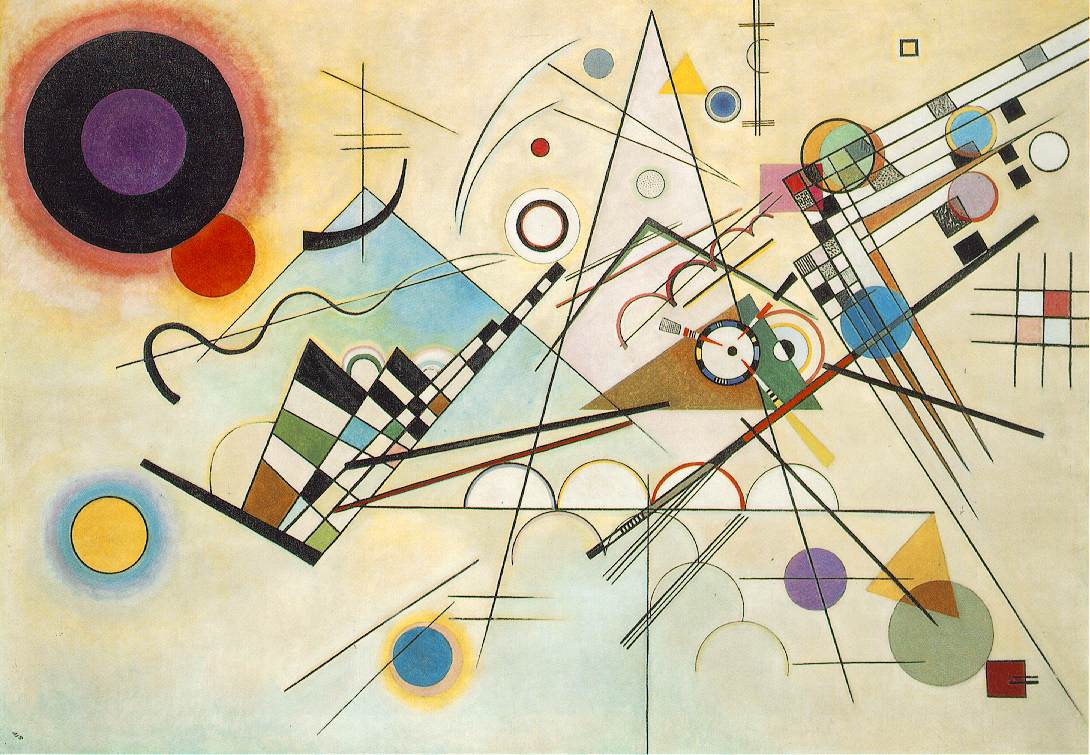
\includegraphics[width=0.75\textwidth]{../images/kandinsky}

%\textsc{\LARGE University of Beer}\\[1.5cm]

%\textsc{\Large Final year project}\\[0.5cm]

% Title
\HRule \\[0.4cm]
{ \Huge \bfseries Applied Data Science}\\[0.4cm]

\HRule \\[1.5cm]

\vspace{2in}
{\LARGE \bfseries Ian Langmore \hfill Daniel Krasner}

% Author and supervisor
%\begin{minipage}{0.4\textwidth}
%\begin{flushleft} \large
%\emph{Author:}\\
%John \textsc{Smith}
%\end{flushleft}
%\end{minipage}
%\begin{minipage}{0.4\textwidth}
%\begin{flushright} \large
%\emph{Supervisor:} \\
%Dr.~Mark \textsc{Brown}
%\end{flushright}
%\end{minipage}

\vfill

% Bottom of the page
%{\large \today}


\end{center}
\end{titlepage}

%\author{}
%\title{Applied Data Science}
%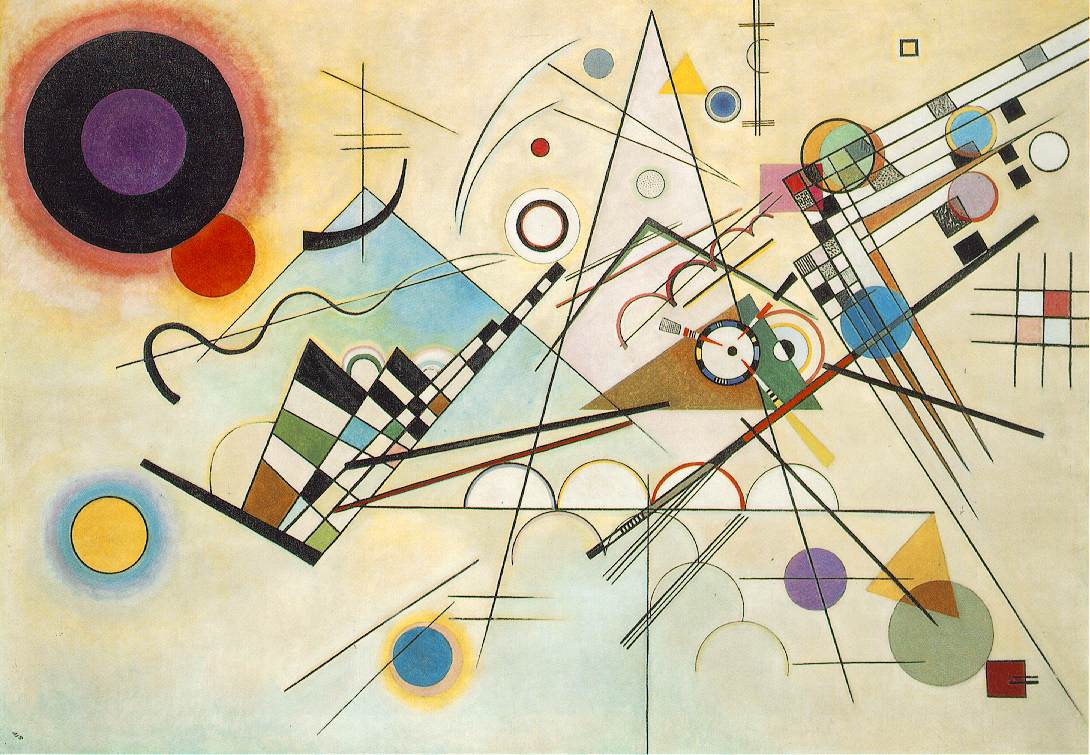
\includegraphics[width=0.5\textwidth]{../images/kandinsky}
%\date{2013}
%\maketitle

\frontmatter
\tableofcontents

\textbf{What is data science?}
With the major technological advances of the last two decades, coupled in part with the internet explosion, a new breed of analysist has emerged. The exact role, background, and skill-set, of a 
\emph{data scientist} are still in the process of being defined and it is likely that by the time you read this some of what we say will seem archaic. 

In very general terms, we view a data scientist as an individual who uses current computational techniques to analyze data.  Now you might make the observation that there is nothing particularly novel 
in this, and subsequenty ask what has forced the definition.\footnote{William S. Cleveland decide to coin the term \emph{data science} and write  \emph{Data Science: An action plan for expanding the technical areas of the field of statistics} \cite{ClevelandData}.  His report outlined six points for a university to follow in developing a data analyst curriculum.}  After all statisticians, physicists, biologisitcs, finance quants, etc have been looking at data since their respective fields 
emerged. 
One short answer comes from the fact that the data sphere has changed and, hence, a new set of skills is 
required to navigate it effectively. The exponential increase in computational power has provided new means to investigate the ever growing amount of data being collected every second of the
day. What this implies is the fact that any modern data analyst will have to make the time investment to learn computational techniques necessary to deal with the volumes and complexity of the data of today.
In addition to those of mathemics and statistics, these software skills are domain transfereable and so it makes sense to create a job title that is also transferable.  We could also point to the ``data hype'' created in industry as a culprit for the term \emph{data science} with the \emph{science} creating an aura of validity and facilitating LinkedIn headhunting.

\textbf{What skills are needed?}
One neat way we like to visualize the data science skill set is with Drew Conway's Venn Diagram\cite{ConwayVenn}, see figure \ref{figure:conwayvenn}.
\begin{figure}
  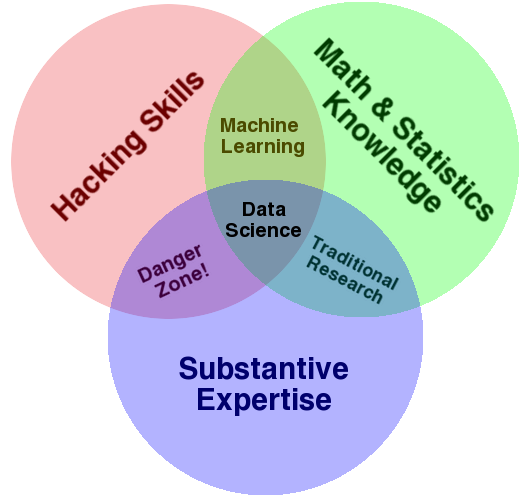
\includegraphics[width=0.5\textwidth]{../images/Data_Science_VD}
  \caption{Drew Conway's Venn Diagram}
  \label{figure:conwayvenn}
\end{figure}
Math and statistics is what allows us to properly quantify a phenomenon observed in data. For the sake of narrative lets take a complex deterministic situation, such as whether or not someone will make a loan payment, 
and attempt to answer this question with a limited number of variables and an imperfect understanding of those variables influence on the event we wish to predict. 
With the exception of your friendly real estate agent we generally acknowldege our lack of soothseer ability and make statements about the probability of this event.  These statements take a mathematical form, for example
\begin{align*}
  \rmP[\mbox{makes-loan-payment}] &= e^{\alpha + \beta\cdot\mbox{creditscore}}.
\end{align*}
where the above quantifies the \emph{risk} associated with this event.  Deciding on the best coefficients $\alpha$ and $\beta$ can be done quite easily by a host of software packages.  In fact anyone with decent hacking
skills can do achieve the goal.  Of course, a simple model such as this would convince no one and would call for substantive expertise (more commonly called \emph{domain knowledge}) to make real progress.  In this case, 
a domain expert would note that additional variables such as the loan to value ratio and housing price index are needed as they have a huge effect on payment activity. These variables and many others 
would allow us to arrive at a  ``better'' model
\begin{align}
  \rmP[\mbox{makes-loan-payment}] &= e^{\alpha + \beta\cdot X}.
  \label{align:preface:logit}
\end{align}
Finally we have arrived at a model capable of fooling someone!  We could keep adding  variables until the model will almost certainly fit the historic risk quite well.  BUT, how do we know that this will allow us to quantify risk in the future? 
To make some sense of our \emph{uncertainty}\footnote{The distrinction between uncertainty and risk has been talked about quite extensively by Nassim Taleb\cite{TalebFooled,TalebBlack}} about our model we need to know eactly what
\eqref{align:preface:logit} means.   In particular, did we include too many variables and \emph{overfit}?  Did our method of solving \eqref{align:preface:logit} arrive at a good solution or just numerical noise?  Most importantly, 
how appropriate is the logistic regression model to begin with?  Answering these questions is often as much an art as a science, but in our experience, sufficient mathematical understanding is necessary to avoid getting lost.


\textbf{What is the motivation for, and focus of, this course?}
Just as common as the hacker with no domain knowledge, or the domain expert with no statistical no-how is the traditional academic with meager computing skills.  Academia rewards papers containing original theory.  For the most part 
it does not reward the considerable effort needed to produce high quality, maintainable code that can be used by others and integrated into larger frameworks.  
As a result, the type of code typically put forward by academics is completely unuseable in industry or by anyone else for that matter. It is often not the purpose or worth the effort to write production level code
in an academic environment. The importance of this cannot be overstated.  Consider a 20 person start-up that wishes to build a smart-phone app that recommends restaurants to users.  
The data scientist hired for this job will need to interact with the company database (they will likely not be handed a neat csv file), deal with falsely entered or inconveniently formatted data, and produce legible reports, 
as well as a working model for the rest of the company to integrate into its production framework. The scientist may be expected to do this work without much in the way of software support.  Now, considering how easy it is to 
blindly run most predictive software, our hypothetical company will be tempted to use a programmer with no statistical knowledge to do this task.  Of course, the programmer will fall into analytic traps such as the ones mentioned above but 
that might not deter anyone from being content with output. This anecdote seems construed, but in reality it is something we have seen time and time again. The current world of data analysis calls for a myriad of skills, 
and clean programming, database interaction and understand of architecture have all become the minimum to succeed. 

The purpose of this course is to take people with strong mathematical/statistical knowledge and teach them software development fundamentals\footnote{Our view of what constitutes the necessary fundamentals is strongly influenced by the team at software carpentry\cite{SWC}}.  This course will cover
\begin{itemize}
  \item Design of small software packages
  \item Working in a Unix environment
  \item Designing software in teams
  \item Fundamental statistical algorithms such as linear and logistic regression
  \item Overfitting and how to avoid it
  \item Working with text data (e.g. regular expressions)
  \item Time series
  \item And more\dots
\end{itemize}



\mainmatter
% \chapter[Unix]{Unix} 
\label{chapter:unix}
\begin{center}
{\Large\textit{Simplicity is the key to brilliance\\-Bruce Lee}}
\end{center}
\vspace{0.2in}

\section{History and Culture} 
\label{unix:history} 
The Unix operating system was developed in 1969 at AT\&T's Bell Labs.  Today Unix lives on through its open source offspring, Linux.  This Operating system the dominant force in scientific computing, super computing, and web servers.  In addition, mac OSX (which is unix based) and a variety of user friendly Linux operating systems represent a significant portion of the personal computer market.  To understand the reasons for this success, some history is needed.

In the 1960s, MIT, AT\&T Bell Labs, and General Electric developed a time-sharing (meaning different users could share one system) operating system called Multics.  Multics was found to be too complicated.  This ``failure'' led researchers to develop a new operating system that focused on simplicity.  This operating system emphasized ease of communication among many simple programs.  Kernighan and Pike summarized this as ``the idea that the power of a system comes more from the relationships among programs than from the programs themselves.''

The Unix community was integrated with the Internet and networked computing from the beginning.  This, along with the solid fundamental design, could have led to Unix becoming the dominant computing paradigm during the 1980's personal computer revolution.  Unfortunately, infighting and poor business decisions kept Unix out of the mainstream.  

Unix found a second life, not so much through better business decisions, but through the efforts of Richard Stallman and GNU Project.  The goal was to produce a Unix-like operating system that depended only on free software.  Free in this case meant, ``users are free to run the software, share it, study it, and modify it.''  The GNU Project succeeded in creating a huge suite of utilities for use with an operating system (e.g. a C compiler) but were lacking the kernel (which handles communication between e.g. hardware and software, or among processes).  It just so happened that Linux Torvalds had developed a kernel (the ``Linux'' kernel) in need of good utilities.  Together the Linux operating system was born.  

\section{The Shell}
Modern Linux distributions, such as Ubuntu, come with a graphical user interface (GUI) every bit as slick as Windows or Mac OSX.  Software is easy to install and with at most a tiny bit of work all non-proprietary applications work fine.  The real power of Unix is realized when you start using the \emph{shell}.
\begin{figure}
  \label{unix:fig:ubuntu}
  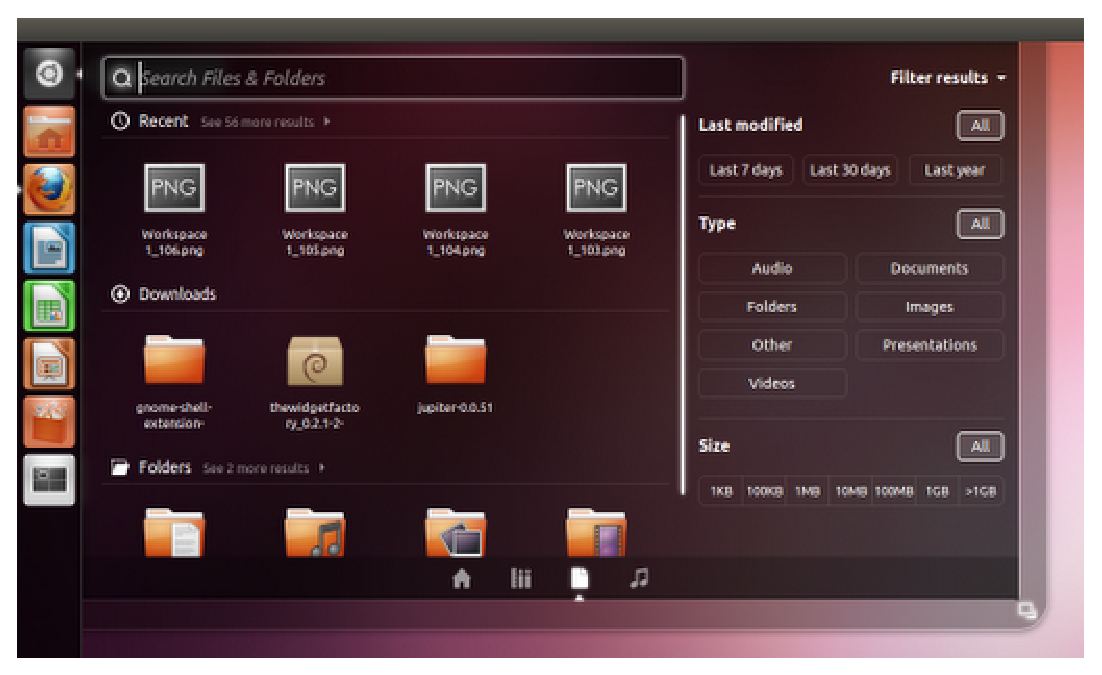
\includegraphics[width=0.5\textwidth]{../images/ubuntugui}
  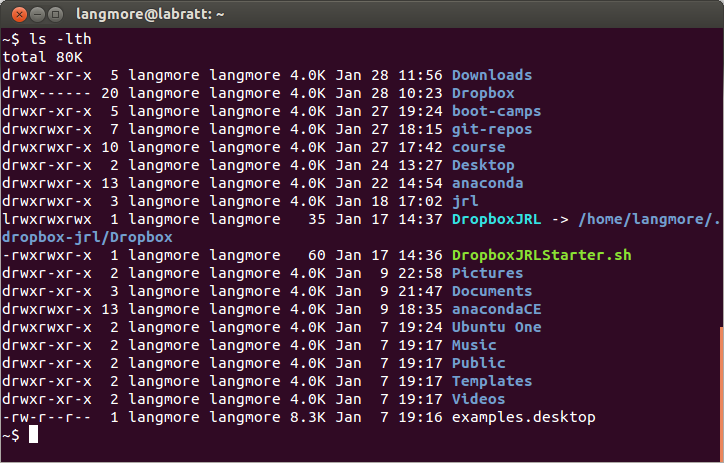
\includegraphics[width=0.5\textwidth]{../images/terminal}
  \caption{Ubuntu's GUI and CLI}
\end{figure}

\begin{digression}[Linux without tears]
  The easiest way to have access to the bash shell and a modern scientific computing environment is to buy hardware that is pre-loaded with Linux.  This way, the hardware vendor is takes responsibility for maintaining the proper drivers.  Use caution when reading blogs talking about how ``easy'' it was to get some off-brand laptop computer working with Linux\ldots this could work for you, or you could be left with a giant headache.  Currently there are a number of hardware vendors that ship machines with Linux:  System76, ZaReason, and Dell (with their ``Project Sputnik'' campaign).  Mac OSX is built on Unix, and also qualifies as a linux machine of sorts.  The disadvantage (of a mac) is price, and the fact that the package management system (for installing software) that comes with Ubuntu linux is the cleanest, easiest ever!
\end{digression}

The shell allows you to control your computer using commands entered in a keyboard.  This sort of interaction is called a \emph{command line interface} (CLI).  ``The shell'' in our case will refer to the \emph{Bourne again} or \emph{bash shell}.  The bash shell provides an interface to your computer's OS along with a number of utilties and minilanguages.  We will introduce you to the shell during the software carpentry bootcamp.  For those unable to attend, we refer you to
% TODO Insert reference

Why learn the shell?
\begin{itemize}
  \item The shell provides a number of utilities that allow you to perform tasks such as interact with your OS or modify a text file.
  \item The shell provides a number \emph{minilanguages} that allow you to automate these tasks.
  \item Often programs must communicate with a user or another machine.  A CLI is a very simple way to do this.  Trust me, you don't want to create a GUI for every script you write.
  \item Usually the only way to communicate with a remote computer/cluster is using a shell.
\end{itemize}

Because of this, programs and workflows that \emph{only} work in the shell are common.  For this reason alone, a modern scientist must learn to use the shell.

Shell utilities have a common format that is almost always adhered to.  This format is:  \T{utilityname  options  arguments}.  The \emph{utilityname} is the name of the utility, such as \T{cut}, which picks out a column of a csv file.  The \emph{options} modify the behavior of the program.  In the case of \T{cut} this could mean specifying how the file is delimited (tabs, spaces, commas, etc\ldots) and which column to pick out.  In general, options should in fact be \emph{optional} in that the utility will work without them (but may not give the desired behavior).  The \emph{arguments} come last.  These are not optional and can often be thought of as the external input to the program.  In the case of \T{cut} this is the file from which to extract a column.  Putting this together, if \T{data.csv} looks like:
\begin{minted}{bash}
  name,age,weight
  ian,1,11
  chang,2,22
\end{minted}
Then
\begin{align}
  &\underbrace{\T{cut}}_\text{utilityname}  \underbrace{\T{-d, -f1}}_\text{options}\quad \underbrace{\T{data.csv}}_\text{arguments}
  \label{unix:align:cut}
\end{align}
produces (more specifically, prints on the terminal screen)
\begin{minted}{bash}
  age
  1
  2
\end{minted}

\section{Streams}
A \emph{stream} is general term for a sequence of data elements made available over time.  This data is processed one element at a time.  For example, consider the data file (which we will call \T{data.csv}):
\begin{minted}{bash}
  name,age,weight
  ian,1,11
  chang,2,22
  daniel,3,33
\end{minted}
This data may exist in one contiguous block in memory/disk or not.  In either case, to process this data as a stream, you should view it as a contiguous block that looks like
\begin{minted}{bash}
  name,age,weight\n ian,1,11\n chang,2,22\n daniel,3,33
\end{minted}
The special character \lstinline$\n$ is called a \emph{newline} character and represents the start of a new line.  The command \T{cut -d, -f2 data.csv} will pick out the second column of \T{data.csv}, in other words, it returns
\begin{minted}{bash}
  age
  1
  2
  3
\end{minted}
, or, thought of as a stream,
\begin{minted}{bash}
  age\n 1\n 2\n 3
\end{minted}
This could be accomplished by reading the file in sequence, starting to store the characters in a buffer once the first comma is hit, then printing when the second comma is hit.  Since the newline is such a special character, many languages provide some means for the user to process each line as a separate item.

This is a very simple way to think about data processing.  This simplicity is advantageous and allows one to scale stream processing to massive scales.  Indeed, the popular Hadoop MapReduce implementation requires that all small tasks operate on streams.  Another advantage of stream processing is that memory needs are reduced.  Programs that are able to read from stdin and write to stdout are known as \emph{filters}.

\subsection{Standard streams}
While stream is a general term, there are three streaming input and output channels available on (almost) every machine.  These are \emph{standard input} (stdin), \emph{standard output} (stdout), and \emph{standard error} (stderr).  Together, these \emph{standard streams} provide a means for a \emph{process} to communicate with other processes, or a computer to communicate with other machines (see figure \ref{unix:fig:stdstreams}).  Standard input is used to allow a process to read data from another source.  A Python programmer could read from standard in, then print the same thing to standard out using
\begin{minted}{python}
for line in sys.stdin:
    sys.stdout.write(line)
\end{minted}
If data is flowing into stdin, then this will result in the same data being written to stdout.  If you launch a terminal, then stdout is (by default) connected to your terminal display.  So if a program sends something to stdout it is displayed on your terminal.  By default stdin is connected to your keyboard.  Stderr operates sort of like stdout but all information carries the special tag, ``this is an error message.''  Stderr is therefore used for printing error/debugging information.
\begin{figure}
  \label{unix:fig:stdstreams}
  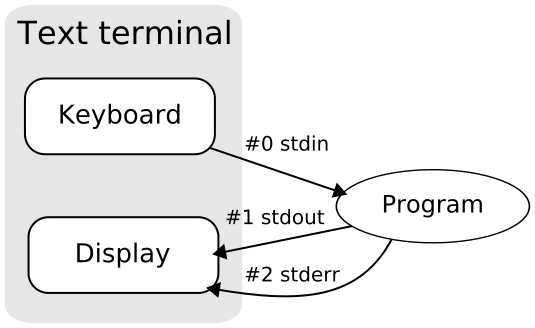
\includegraphics[width=0.7\textwidth]{../images/Stdstreams-notitle}
  \caption{Illustration of the standard streams}
\end{figure}


\subsection{Pipes}
\label{subsection:pipes}
The standard streams aren't any good if there isn't any way to access them.  Unix provides a very simple means to connect the standard output of one process to the standard input of another.  This construct called a \emph{pipe} and is written with a vertical bar \T{|}.  Utilities tied together with pipes form what is known as a \emph{pipeline}.

Consider the following pipeline
\begin{minted}{bash}
  \$ cat infile.csv | cut -d, -f1 | sort | uniq -c
\end{minted}
The above line reads in a text file and prints it to standard out with \T{cat}, the pipe ``\textbar'' redirects this standard out to the standard in of \T{cut}.  \T{cut} in turn extracts the first column and passes the result to \T{sort}, which sends its result to \T{uniq}.  \T{uniq -c} counts the number of unique occurrences of each word.

Let's decompose this step-by-step:  First, print \emph{infile.csv} to stdout (which is, by default, the terminal) using cat.
\begin{minted}{bash}
  \$ cat infile.csv

  ian,1
  daniel,2
  chang,3
  ian,11
\end{minted}
Second, pipe this to \T{cut}, which will extract the first \emph{field} (the \T{-f} option) in this comma delimited (the \T{-d,} option) file. 
\begin{minted}{bash}
  \$ cat infile.csv | cut -d, -f1

  ian
  daniel
  chang
  ian
\end{minted}
Third, pipe the output of cut to sort
\begin{minted}{bash}
  \$ cat infile.csv | cut -d, -f1 | sort

  chang
  daniel
  ian
  ian
\end{minted}
Third, redirect the output of sort to uniq.
\begin{minted}{bash}
  \$ cat infile.csv | cut -d, -f1 | sort | uniq -c

  1  chang
  1  daniel
  2  ian
\end{minted}
It is important to note that uniq counts unique occurrences in consecutive lines of text.  If we did not sort the input to uniq, we would have
\begin{minted}{bash}
  \$ cat infile.csv | cut -d, -f1 | uniq -c

  1  ian
  1  daniel
  1  chang
  1  ian
\end{minted}
\T{uniq} processes text streams character-by-character and does not have the ability to look ahead and see that ``ian'' will occur a second time.


\section{Text}
One surprising thing to some Unix newcomers is the degree to which simple plain text dominates.  The preferred file format for most data files and streams is just plain text.  

Why not use a compressed binary format that would be quicker to read/write using a special reader application?  The reason is in the question:  A special reader application would be needed.  As time goes on, many data formats and reader applications come in, and then out of favor.  Soon your special format data file needs a hard to find application to read it\footnote{Any user of Microsoft Word documents from the 90's should be familiar with the headaches that can arise from this situation.}.  What about for communication between processes on a machine?  The same situation arises:  As soon as more than one binary format is used, it is possible for one of them to become obsolete.  Even if both are well supported, every process needs to specify what format it is using.  Another advantage of working with text streams is the fact that humans can visually inspect them for debugging purposes.

While binary formats live and die on a quick (computer) time-scale, change in human languages changes on the scale of at least a generation.  In fact, one summary of the Unix philosophy goes, ``This is the Unix philosophy: Write programs that do one thing and do it well. Write programs to work together. Write programs to handle text streams, because that is a universal interface.''

This, in addition to the fact that programming in general requires manipulation of text files, means that you are required to master decent text processing software.  Here is a brief overview of some popular programs
\begin{itemize}
  \item {\bf Vim} is a powerful text editor designed to allow quick editing of files and minimal hand movement.
  \item {\bf Emacs} is another powerful text editor.  Some people find that it requires users to contort their hands and leads to wrist problems.
  \item {\bf Gedit, sublime text} are decent text editors available for Linux and Mac.  They are not as powerful as Vim/Emacs, but don't require any special skills to use.
  \item {\bf nano} is a simple unix text editor available on any system.  If nano doesn't work, try \emph{pico}.
  \item {\bf sed} is a text stream processing command line utility available in your shell.  It can do simple operations on one line of text at a time.  It is useful because of its speed, and the fact that it can handle arbitrarily large files.
  \item {\bf awk} is an old school minilanguage that allows more complex operations than sed.  It is often acknowledged that awk syntax is too complex and that learning to write simple Python scripts is a better game plan.
\end{itemize}
\section{Philosophy}
The Unix culture carries with it a philosophy about software design.  The Unix operating system (and its core utilities) can be seen as examples of this.    Let's go over some key rules.  With the exception of the rule of collaboration, these appeared previously in \cite{RaymondUnix}.

\subsection{In a nutshell}

\vspace{0.1in}
\noindent\textit{\textbf{Rule of Simplicity.}}
Design for simplicity.  Add complexity only when you must.

\vspace{0.1in}
\noindent\textit{\textbf{Rule of Collaboration.}}
Make programs that work together.  Work together with people to make programs

\subsection{More nuts and bolts}

We can add more rules to the two main rules above, and provide hints as to how they will guide our software development.  Our programs will be small, so (hopefully) few compromises will have to be made.

\textit{\textbf{Rule of Simplicity.}}
This is sometimes expressed as K.I.S.S, or ``Keep It Simple Stupid.''  All other philosophical points presented here can be seen as special cases of this.  Complex programs are difficult to debug, implement, maintain, or extend.  We will keep things simple by, for example:
(i) writing CLI utilities that \emph{do one thing well},
(ii) avoiding objects unless using them results in a simpler, more transparent design,
and
(iii) in our modules, include only features that will be used right now.

\textit{\textbf{Rule of Collaboration.}}
We will make programs that work together by, for example:
(i) writing CLI utilities that work as filters,
and
(ii) choosing common data structures (such as Numpy arrays, Pandas DataFrames).
We will work together with people to make programs by, for example:
(i) employing Git as a version control system (using Github to host our code)
and,
(ii) enforcing code readability standards such as PEP8.

\textit{\textbf{Rule of Modularity.}}
Write simple parts connected by clean interfaces.  Humans can hold only a limited amount of information in their head at one time.  Make your functions small (simple) enough so that they can be explained in one sentence.

\textit{\textbf{Rule of Clarity.}}
Clarity is better than cleverness.  Maintenance and debugging of code is very expensive.  Take time to make sure your program logic will be clear to someone reading your code some time in the future (this person might be you).  Comments are important.  Better yet, code can often be written to read like a story\dots and no comments are necessary.
\begin{minted}{python}
  for row in reader:
      rowsum = sum_row(row)
      row.append(rowsum)
      writer.write(row)
\end{minted}

\textit{\textbf{Rule of Composition.}}
Design programs to be connected to other programs.  The Unix command line utilities are an example of this.  They (typically) can read from a file or stdin, and write to stdout.  Thus, multiple utilities can be tied together with pipes.
\begin{minted}{bash}
  cat infile.csv | cut -f1 | sort | uniq -c
\end{minted}


\textit{\textbf{Rule of Least Surprise.}}
Try to do the least surprising thing.  We will follow Unix or Python convention whenever possible.  For example, our data files will be in common formats such as csv, xml, json, etc\dots


\section{End Notes}
\emph{Revolution OS} is a fun movie about the rise of Linux.

\cite{RaymondUnix} gives a comprehensive exposition of the history and philosophy of Unix, and provides most of the material you see in our history and philosophy sections.  

The quote by Kernighan and Pike can be found in ``The Unix programming environment.''\cite{UnixProgrammingEnvironment}

Software Carpentry held a bootcamp for students in three courses at Columbia University in 2013 \cite{SWC-NYC2013}.

The impact of the inventions to come out of Bell Labs cannot be understated.  Also developed there were radio astronomy, the transistor, the laser, the CCD, information theory, and the C/C++ programming languages.\cite{BellLabsWikipedia}
 means that unix.tex will be inserted verbatim into this file.
\part{Programming Prerequisites}
\chapter[Unix]{Unix} 
\label{chapter:unix}
\begin{center}
{\Large\textit{Simplicity is the key to brilliance\\-Bruce Lee}}
\end{center}
\vspace{0.2in}

\section{History and Culture} 
\label{unix:history} 
The Unix operating system was developed in 1969 at AT\&T's Bell Labs.  Today Unix lives on through its open source offspring, Linux.  This Operating system the dominant force in scientific computing, super computing, and web servers.  In addition, mac OSX (which is unix based) and a variety of user friendly Linux operating systems represent a significant portion of the personal computer market.  To understand the reasons for this success, some history is needed.

In the 1960s, MIT, AT\&T Bell Labs, and General Electric developed a time-sharing (meaning different users could share one system) operating system called Multics.  Multics was found to be too complicated.  This ``failure'' led researchers to develop a new operating system that focused on simplicity.  This operating system emphasized ease of communication among many simple programs.  Kernighan and Pike summarized this as ``the idea that the power of a system comes more from the relationships among programs than from the programs themselves.''

The Unix community was integrated with the Internet and networked computing from the beginning.  This, along with the solid fundamental design, could have led to Unix becoming the dominant computing paradigm during the 1980's personal computer revolution.  Unfortunately, infighting and poor business decisions kept Unix out of the mainstream.  

Unix found a second life, not so much through better business decisions, but through the efforts of Richard Stallman and GNU Project.  The goal was to produce a Unix-like operating system that depended only on free software.  Free in this case meant, ``users are free to run the software, share it, study it, and modify it.''  The GNU Project succeeded in creating a huge suite of utilities for use with an operating system (e.g. a C compiler) but were lacking the kernel (which handles communication between e.g. hardware and software, or among processes).  It just so happened that Linux Torvalds had developed a kernel (the ``Linux'' kernel) in need of good utilities.  Together the Linux operating system was born.  

\section{The Shell}
Modern Linux distributions, such as Ubuntu, come with a graphical user interface (GUI) every bit as slick as Windows or Mac OSX.  Software is easy to install and with at most a tiny bit of work all non-proprietary applications work fine.  The real power of Unix is realized when you start using the \emph{shell}.
\begin{figure}
  \label{unix:fig:ubuntu}
  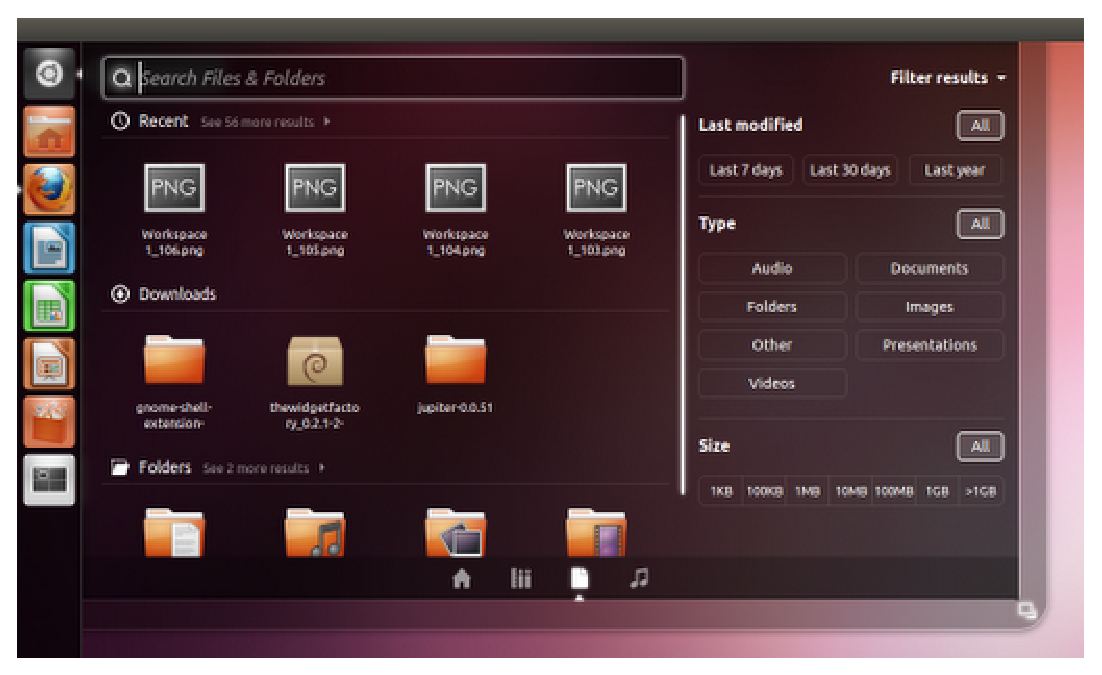
\includegraphics[width=0.5\textwidth]{../images/ubuntugui}
  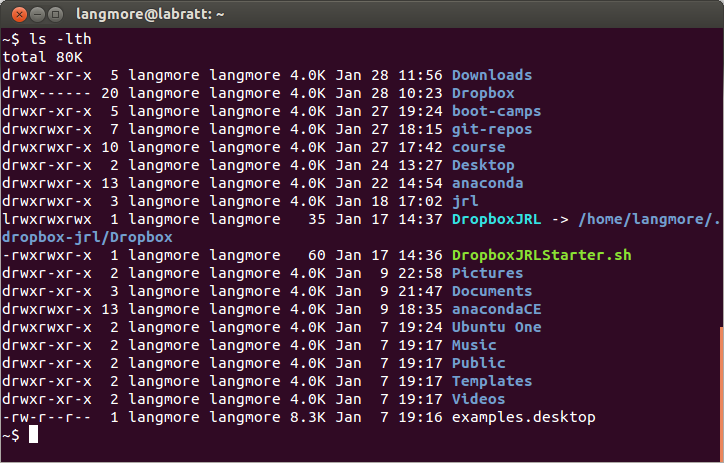
\includegraphics[width=0.5\textwidth]{../images/terminal}
  \caption{Ubuntu's GUI and CLI}
\end{figure}

\begin{digression}[Linux without tears]
  The easiest way to have access to the bash shell and a modern scientific computing environment is to buy hardware that is pre-loaded with Linux.  This way, the hardware vendor is takes responsibility for maintaining the proper drivers.  Use caution when reading blogs talking about how ``easy'' it was to get some off-brand laptop computer working with Linux\ldots this could work for you, or you could be left with a giant headache.  Currently there are a number of hardware vendors that ship machines with Linux:  System76, ZaReason, and Dell (with their ``Project Sputnik'' campaign).  Mac OSX is built on Unix, and also qualifies as a linux machine of sorts.  The disadvantage (of a mac) is price, and the fact that the package management system (for installing software) that comes with Ubuntu linux is the cleanest, easiest ever!
\end{digression}

The shell allows you to control your computer using commands entered in a keyboard.  This sort of interaction is called a \emph{command line interface} (CLI).  ``The shell'' in our case will refer to the \emph{Bourne again} or \emph{bash shell}.  The bash shell provides an interface to your computer's OS along with a number of utilties and minilanguages.  We will introduce you to the shell during the software carpentry bootcamp.  For those unable to attend, we refer you to
% TODO Insert reference

Why learn the shell?
\begin{itemize}
  \item The shell provides a number of utilities that allow you to perform tasks such as interact with your OS or modify a text file.
  \item The shell provides a number \emph{minilanguages} that allow you to automate these tasks.
  \item Often programs must communicate with a user or another machine.  A CLI is a very simple way to do this.  Trust me, you don't want to create a GUI for every script you write.
  \item Usually the only way to communicate with a remote computer/cluster is using a shell.
\end{itemize}

Because of this, programs and workflows that \emph{only} work in the shell are common.  For this reason alone, a modern scientist must learn to use the shell.

Shell utilities have a common format that is almost always adhered to.  This format is:  \T{utilityname  options  arguments}.  The \emph{utilityname} is the name of the utility, such as \T{cut}, which picks out a column of a csv file.  The \emph{options} modify the behavior of the program.  In the case of \T{cut} this could mean specifying how the file is delimited (tabs, spaces, commas, etc\ldots) and which column to pick out.  In general, options should in fact be \emph{optional} in that the utility will work without them (but may not give the desired behavior).  The \emph{arguments} come last.  These are not optional and can often be thought of as the external input to the program.  In the case of \T{cut} this is the file from which to extract a column.  Putting this together, if \T{data.csv} looks like:
\begin{minted}{bash}
  name,age,weight
  ian,1,11
  chang,2,22
\end{minted}
Then
\begin{align}
  &\underbrace{\T{cut}}_\text{utilityname}  \underbrace{\T{-d, -f1}}_\text{options}\quad \underbrace{\T{data.csv}}_\text{arguments}
  \label{unix:align:cut}
\end{align}
produces (more specifically, prints on the terminal screen)
\begin{minted}{bash}
  age
  1
  2
\end{minted}

\section{Streams}
A \emph{stream} is general term for a sequence of data elements made available over time.  This data is processed one element at a time.  For example, consider the data file (which we will call \T{data.csv}):
\begin{minted}{bash}
  name,age,weight
  ian,1,11
  chang,2,22
  daniel,3,33
\end{minted}
This data may exist in one contiguous block in memory/disk or not.  In either case, to process this data as a stream, you should view it as a contiguous block that looks like
\begin{minted}{bash}
  name,age,weight\n ian,1,11\n chang,2,22\n daniel,3,33
\end{minted}
The special character \lstinline$\n$ is called a \emph{newline} character and represents the start of a new line.  The command \T{cut -d, -f2 data.csv} will pick out the second column of \T{data.csv}, in other words, it returns
\begin{minted}{bash}
  age
  1
  2
  3
\end{minted}
, or, thought of as a stream,
\begin{minted}{bash}
  age\n 1\n 2\n 3
\end{minted}
This could be accomplished by reading the file in sequence, starting to store the characters in a buffer once the first comma is hit, then printing when the second comma is hit.  Since the newline is such a special character, many languages provide some means for the user to process each line as a separate item.

This is a very simple way to think about data processing.  This simplicity is advantageous and allows one to scale stream processing to massive scales.  Indeed, the popular Hadoop MapReduce implementation requires that all small tasks operate on streams.  Another advantage of stream processing is that memory needs are reduced.  Programs that are able to read from stdin and write to stdout are known as \emph{filters}.

\subsection{Standard streams}
While stream is a general term, there are three streaming input and output channels available on (almost) every machine.  These are \emph{standard input} (stdin), \emph{standard output} (stdout), and \emph{standard error} (stderr).  Together, these \emph{standard streams} provide a means for a \emph{process} to communicate with other processes, or a computer to communicate with other machines (see figure \ref{unix:fig:stdstreams}).  Standard input is used to allow a process to read data from another source.  A Python programmer could read from standard in, then print the same thing to standard out using
\begin{minted}{python}
for line in sys.stdin:
    sys.stdout.write(line)
\end{minted}
If data is flowing into stdin, then this will result in the same data being written to stdout.  If you launch a terminal, then stdout is (by default) connected to your terminal display.  So if a program sends something to stdout it is displayed on your terminal.  By default stdin is connected to your keyboard.  Stderr operates sort of like stdout but all information carries the special tag, ``this is an error message.''  Stderr is therefore used for printing error/debugging information.
\begin{figure}
  \label{unix:fig:stdstreams}
  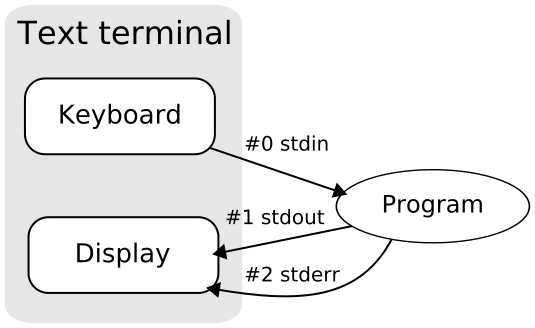
\includegraphics[width=0.7\textwidth]{../images/Stdstreams-notitle}
  \caption{Illustration of the standard streams}
\end{figure}


\subsection{Pipes}
\label{subsection:pipes}
The standard streams aren't any good if there isn't any way to access them.  Unix provides a very simple means to connect the standard output of one process to the standard input of another.  This construct called a \emph{pipe} and is written with a vertical bar \T{|}.  Utilities tied together with pipes form what is known as a \emph{pipeline}.

Consider the following pipeline
\begin{minted}{bash}
  \$ cat infile.csv | cut -d, -f1 | sort | uniq -c
\end{minted}
The above line reads in a text file and prints it to standard out with \T{cat}, the pipe ``\textbar'' redirects this standard out to the standard in of \T{cut}.  \T{cut} in turn extracts the first column and passes the result to \T{sort}, which sends its result to \T{uniq}.  \T{uniq -c} counts the number of unique occurrences of each word.

Let's decompose this step-by-step:  First, print \emph{infile.csv} to stdout (which is, by default, the terminal) using cat.
\begin{minted}{bash}
  \$ cat infile.csv

  ian,1
  daniel,2
  chang,3
  ian,11
\end{minted}
Second, pipe this to \T{cut}, which will extract the first \emph{field} (the \T{-f} option) in this comma delimited (the \T{-d,} option) file. 
\begin{minted}{bash}
  \$ cat infile.csv | cut -d, -f1

  ian
  daniel
  chang
  ian
\end{minted}
Third, pipe the output of cut to sort
\begin{minted}{bash}
  \$ cat infile.csv | cut -d, -f1 | sort

  chang
  daniel
  ian
  ian
\end{minted}
Third, redirect the output of sort to uniq.
\begin{minted}{bash}
  \$ cat infile.csv | cut -d, -f1 | sort | uniq -c

  1  chang
  1  daniel
  2  ian
\end{minted}
It is important to note that uniq counts unique occurrences in consecutive lines of text.  If we did not sort the input to uniq, we would have
\begin{minted}{bash}
  \$ cat infile.csv | cut -d, -f1 | uniq -c

  1  ian
  1  daniel
  1  chang
  1  ian
\end{minted}
\T{uniq} processes text streams character-by-character and does not have the ability to look ahead and see that ``ian'' will occur a second time.


\section{Text}
One surprising thing to some Unix newcomers is the degree to which simple plain text dominates.  The preferred file format for most data files and streams is just plain text.  

Why not use a compressed binary format that would be quicker to read/write using a special reader application?  The reason is in the question:  A special reader application would be needed.  As time goes on, many data formats and reader applications come in, and then out of favor.  Soon your special format data file needs a hard to find application to read it\footnote{Any user of Microsoft Word documents from the 90's should be familiar with the headaches that can arise from this situation.}.  What about for communication between processes on a machine?  The same situation arises:  As soon as more than one binary format is used, it is possible for one of them to become obsolete.  Even if both are well supported, every process needs to specify what format it is using.  Another advantage of working with text streams is the fact that humans can visually inspect them for debugging purposes.

While binary formats live and die on a quick (computer) time-scale, change in human languages changes on the scale of at least a generation.  In fact, one summary of the Unix philosophy goes, ``This is the Unix philosophy: Write programs that do one thing and do it well. Write programs to work together. Write programs to handle text streams, because that is a universal interface.''

This, in addition to the fact that programming in general requires manipulation of text files, means that you are required to master decent text processing software.  Here is a brief overview of some popular programs
\begin{itemize}
  \item {\bf Vim} is a powerful text editor designed to allow quick editing of files and minimal hand movement.
  \item {\bf Emacs} is another powerful text editor.  Some people find that it requires users to contort their hands and leads to wrist problems.
  \item {\bf Gedit, sublime text} are decent text editors available for Linux and Mac.  They are not as powerful as Vim/Emacs, but don't require any special skills to use.
  \item {\bf nano} is a simple unix text editor available on any system.  If nano doesn't work, try \emph{pico}.
  \item {\bf sed} is a text stream processing command line utility available in your shell.  It can do simple operations on one line of text at a time.  It is useful because of its speed, and the fact that it can handle arbitrarily large files.
  \item {\bf awk} is an old school minilanguage that allows more complex operations than sed.  It is often acknowledged that awk syntax is too complex and that learning to write simple Python scripts is a better game plan.
\end{itemize}
\section{Philosophy}
The Unix culture carries with it a philosophy about software design.  The Unix operating system (and its core utilities) can be seen as examples of this.    Let's go over some key rules.  With the exception of the rule of collaboration, these appeared previously in \cite{RaymondUnix}.

\subsection{In a nutshell}

\vspace{0.1in}
\noindent\textit{\textbf{Rule of Simplicity.}}
Design for simplicity.  Add complexity only when you must.

\vspace{0.1in}
\noindent\textit{\textbf{Rule of Collaboration.}}
Make programs that work together.  Work together with people to make programs

\subsection{More nuts and bolts}

We can add more rules to the two main rules above, and provide hints as to how they will guide our software development.  Our programs will be small, so (hopefully) few compromises will have to be made.

\textit{\textbf{Rule of Simplicity.}}
This is sometimes expressed as K.I.S.S, or ``Keep It Simple Stupid.''  All other philosophical points presented here can be seen as special cases of this.  Complex programs are difficult to debug, implement, maintain, or extend.  We will keep things simple by, for example:
(i) writing CLI utilities that \emph{do one thing well},
(ii) avoiding objects unless using them results in a simpler, more transparent design,
and
(iii) in our modules, include only features that will be used right now.

\textit{\textbf{Rule of Collaboration.}}
We will make programs that work together by, for example:
(i) writing CLI utilities that work as filters,
and
(ii) choosing common data structures (such as Numpy arrays, Pandas DataFrames).
We will work together with people to make programs by, for example:
(i) employing Git as a version control system (using Github to host our code)
and,
(ii) enforcing code readability standards such as PEP8.

\textit{\textbf{Rule of Modularity.}}
Write simple parts connected by clean interfaces.  Humans can hold only a limited amount of information in their head at one time.  Make your functions small (simple) enough so that they can be explained in one sentence.

\textit{\textbf{Rule of Clarity.}}
Clarity is better than cleverness.  Maintenance and debugging of code is very expensive.  Take time to make sure your program logic will be clear to someone reading your code some time in the future (this person might be you).  Comments are important.  Better yet, code can often be written to read like a story\dots and no comments are necessary.
\begin{minted}{python}
  for row in reader:
      rowsum = sum_row(row)
      row.append(rowsum)
      writer.write(row)
\end{minted}

\textit{\textbf{Rule of Composition.}}
Design programs to be connected to other programs.  The Unix command line utilities are an example of this.  They (typically) can read from a file or stdin, and write to stdout.  Thus, multiple utilities can be tied together with pipes.
\begin{minted}{bash}
  cat infile.csv | cut -f1 | sort | uniq -c
\end{minted}


\textit{\textbf{Rule of Least Surprise.}}
Try to do the least surprising thing.  We will follow Unix or Python convention whenever possible.  For example, our data files will be in common formats such as csv, xml, json, etc\dots


\section{End Notes}
\emph{Revolution OS} is a fun movie about the rise of Linux.

\cite{RaymondUnix} gives a comprehensive exposition of the history and philosophy of Unix, and provides most of the material you see in our history and philosophy sections.  

The quote by Kernighan and Pike can be found in ``The Unix programming environment.''\cite{UnixProgrammingEnvironment}

Software Carpentry held a bootcamp for students in three courses at Columbia University in 2013 \cite{SWC-NYC2013}.

The impact of the inventions to come out of Bell Labs cannot be understated.  Also developed there were radio astronomy, the transistor, the laser, the CCD, information theory, and the C/C++ programming languages.\cite{BellLabsWikipedia}

\chapter{Version Control with Git}
\label{chapter:git}
\begin{center}
{\Large\textit{Git!  That's the vcs that I have to look at Google to use.\\- Josef Perktold}}
\end{center}
\vspace{0.2in}

\section{Background}
\label{git:whatis_vcs}

The idea of version control is almost as old as writing itself. Authors writing books and manuscripts all needed logical ways to keep track of the various edits they made throughout the writing process.  Version control systems like Git, SVN, Mercurial, or CVS allow you to save different versions of your files, and revert to those earlier versions when necessary.  The most modern of these four systems are Git and Mercurial.  Each of these have many features designed to facilitate working in large groups and keeping track of many versions of files.

\section{What is Git}
\label{git:whatis_git}

Git is a distributed version control system (DVCS). This means that every user has a complete copy of the repository on their machine.  This is nice, since you don't need an internet connection to check out different versions of your code, or save a new version.  Multiple users still do need some way to share files.  In this class we will use Git along with the website GitHub.  GitHub provides you with a clone of your local repository that is accessible via the internet.  Thus, when you change a file you will \emph{push} those changes to GitHub, and then your teammates will \emph{pull} those changes down to their local machines.

\section{Setting Up}
\label{git:setting_up}
For macs, download from \url{mac.github.com}.  For Linux, type \T{sudo apt-get install git}.  After installation, get an account at \url{www.github.com}.  Then, in your home directory create a file (or edit if it already exists) called \T{.gitconfig}.  It should have the lines:

\begin{minted}{bash}
[user]
    name = Ian Langmore
    email = ianlangmore@gmail.com
[credential]
    helper = cache --timeout=3600
[alias]
        lol = log --graph --decorate --pretty=oneline --abbrev-commit
        lola = log --graph --decorate --pretty=oneline --abbrev-commit --all
[color]
        branch = auto
        diff = auto
        interactive = auto
        status = auto
\end{minted}

Now, when you're in a repository, you can see the project structure by typing \T{git lola}.

\section{Online Materials}
\label{git:online_materials}
Lots of materials are available online.  Here we list a few.  Be advised that these tutorials are usually written for experienced developers who are migrating from other systems to Git.  For example, in this class you will not have to use branches.

\begin{itemize}
  \item \url{http://git-scm.com/book} has complete documentation with examples.  I recommend reading section 1 before proceeding.
  \item \url{http://osteele.com/posts/2008/05/commit-policies} is a visualization of how to transport data over the multiple layers of Git.
  \item \url{http://marklodato.github.com/visual-git-guide/index-en.html} provides a more complete visual reference.
  \item \url{http://learn.github.com} has a number of video tutorials
  \item \url{http://www.kernel.org/pub/software/scm/git/docs/user-manual.html} is a reference for commands
\end{itemize}

\section{Basic Git Concepts}
\label{git:concepts}
One difficulty that beginners have with Git is understanding that as you are working on a file, there are at least four different versions of it.
\begin{enumerate}
  \item The \emph{working-copy} that is saved in your computer's file system.
  \item The saved version in Git's \emph{index} (a.k.a. \emph{staging area}).  This is where Git keeps the files that will be committed.
  \item The commit current at your \emph{HEAD}.  Once you commit a file, it (and the other files committed with it) are saved forever.  The commit can be identified by a SHA1 hashtag.  The last commit in the current checked out branch is called HEAD.
  \item The commit in your \emph{remote repository}.  Once you have pulled down changes from the remote repository, and pushed your changes to it, your repository is identical to the remote.
\end{enumerate}



\section{Common Git Workflows}
\label{git:workflows}
Here we describe common workflows and the steps needed to execute them.  You can test out the steps here (except the remote steps) by creating a temporary local repository:

\begin{minted}{bash}
  cd /tmp
  mkdir repo
  cd repo
  git init
\end{minted}
After that you will probably want to quickly create a file and add it to the repo.  Do this with
\begin{minted}{bash}
  echo 'line1' > file
  git add file
\end{minted}
Practice this (and subsequent subsections) on your own.  Remember to type \T{git lola}, \T{git status}, and \T{git log} frequently to see what is happening.

You can then add other lines with e.g. \T{echo 'line2' >> file}.  When you are done, you can clean up with \T{rm -rf repo}.

To set up a remote repository on GitHub, follow the directions at: \url{https://help.github.com/articles/creating-a-new-repository}.

\subsection{Linear Move from Working to Remote}
To turn in homework, you have to move files from 1 to 4.  The basic 1-to-4 workflow would be (note that I use \T{<something>} when you must fill in some obvious replacement for the word ``something.''  If the ``something'' is optional I write it in \T{[square brackets]}).
\begin{itemize}
  \item {\bf working-copy $\to$ index} \T{git add <file>}.  To see the files that differ in index and commit use \T{git status}.  To see the differences between working and index files, use \T{git diff [<file>]}.
  \item {\bf index $\to$ HEAD} \T{git commit -m "<message>"}.  To see the files that differ in index and commit use \T{git status}.  To see the differences between your working-copy and the commit, use \T{git diff HEAD [<file>]}.
  \item {\bf HEAD $\to$ remote-repo} \T{git push [origin master]}.  This means ``push the commits in your master branch to the remote repo named origin.''  Note that \T[origin master] is the default, so it isn't necessary.  This actually pushes all commits to origin, but in particular it pushes HEAD.
\end{itemize}

You can add and commit at once with \T{git commit -am '<message>'}.  This will add files that have been previously added.  It will not add untracked files (you have to manually add them with \T{git add <file>}).

\subsection{Discarding changes in your working copy}
You can replace your working copy with the copy in your index using
\begin{minted}{bash}
  git checkout <file>
\end{minted}

You can replace your working copy with the copy in HEAD using
\begin{minted}{bash}
  git checkout HEAD <file>
\end{minted}

\subsection{Erasing changes}
If you committed something you shouldn't have, and want to completely wipe out the commit:
\T{git reset --hard HEAD$^\wedge$}.  This moves your commit back in history and wipes out the most recent commit.

To move the index and HEAD back one commit, use \T{git reset HEAD$^\wedge$}.  

To move the index to a certain commit (designated by a SHA1 hash), use \T{git reset <hash>}.

If you then want to move changes into your working copy, use \T{git checkout <filename>}.

To move contents of a particular commit into your working directory, use \T{git checkout <hash> [<filename>]}.

\subsection{Remotes}
To copy a remote repository, use one of the following
\begin{minted}{bash}
  git clone <remote url>
  git clone <remote url> -b <branchname>
  git clone <remote url> -b <branchname> <destination>
\end{minted}

To get changes from a remote repository and put them into your repo/index/working, use \T{git pull}.  You will get an error if you have uncommitted changes in your index or working, so first save your changes, then \T{git add <filename>}, then \T{git commit -m '<message>'}.

To send changes to a remote repository, use 
\begin{minted}{bash}
  git add <file>
  git commit '<message>'
  git push
\end{minted}

\subsection{Merge conflicts}
A typical situation is as follows:
\begin{enumerate}
  \item Your teammate modifies \T{<file>}
  \item Your teammate pushes changes
  \item You modify \T{<file>}
  \item You pull with \T{git pull}
\end{enumerate}
Git will recognize that you have two versions of the same file that are in ``conflict.''  Git will tell you which files are in conflict.  You can open these files and see something like the following:
\begin{minted}{bash}
  <<<<<<< HEAD:filename
  <My work>
=======
  <My teammate's work>
>>>>>>> iss53:filename
\end{minted}

The lines above the \T{=======} are the version in the commit you most recently made.  The lines below are those in your teammate's version.  You can do a few things:

\begin{itemize}
  \item Edit the file, by hand, to get in in the state you want it in.
  \item Keep your version with \T{git checkout --ours <filename>}
  \item Keep their version with \T{git checkout --theirs <filename>}
\end{itemize}

\chapter{Building a Data Cleaning Pipeline with Python}
\label{chapter:pythonpipeline}
\begin{center}
{\Large\textit{A quotation}}
\end{center}
\vspace{0.2in}

One of the most useful things you can do with Python is to (quickly) build CLI utilities that look and feel like standard Unix tools.  These utilities can be tied together, using pipes and a shell script, into a \emph{pipeline}.  These can be used for many purposes.  We will concentrate on the task of data cleaning or data preparation.


\section{Simple Shell Scripts}
A pipeline that sorts and cleans data could be put into a shell script that looks like:
\begin{minted}{bash}
#!/bin/bash

# Here is a comment

SRC=../src
DATA=../data

cat $DATA/inputfile.csv \
    | python $SRC/subsample.py -r 0.1 \
    | python $SRC/cleandata.py \
    > $DATA/outputfile.csv
\end{minted}
Some points:
\begin{itemize}
  \item The \#\T{!/bin/bash} is called a \emph{she-bang} and in this case tells your machine to run this script using the command \T{/bin/bash}.  In other words, let bash run this script.  
  \item All other lines starting with \# are comments.
  \item The line \T{SRC=../src} sets a variable, \T{SRC}, to the string \T{../src}.  In this case we are referring to a directory containing our source code.  To access the value stored in this variable, we use \$\T{SRC}.  
  \item The lines that end with a backslash \textbackslash, are in fact interpreted as one long line with no newlines.  This is done to improve readability.  
  \item The first couple lines under \T{cat} start with pipes, and the last line is a redirection.  
  \item The command \T{cat} is used on the first line and the output is piped to the first program.  This is done rather than simply using (as the first line) \T{python \$SRC/subsample.py -r 0.1 \$DATA/inputfile.csv}.  What advantage does this give?  It allows one to easily substitute \T{head} for \T{cat} and have a program that reads only the first 10 lines.  This is useful for debugging.
\end{itemize}

Why write shell scripts to run you programs?  
\begin{itemize}
  \item Shell scripts allow you to tie together any program that reads from stdin and writes to stdout.  This includes all the existing Unix utilities.
  \item You can (and should) add the shell scripts to your repository.  This keeps a record of how data was generated.
  \item Anyone who understands Unix will be able to understand how your data was generated.
  \item If your script pipes together five programs, then all five can run at once.  This is a simple way to parallelize things.
  \item More complex scripts can be written that can automate this process
\end{itemize}

\section{Template for a Python CLI Utility}
Python can be written to work as a filter.  To demonstrate, we write a program that would delete every $n^{th}$ line of a file.

\rule{\textwidth}{2pt}
\begin{minted}{python}
from optparse import OptionParser
import sys


def main():
    r"""
    DESCRIPTION
    -----------
    Deletes every nth line of a file or stdin, starting with the
    first line, print to stdout.

    EXAMPLES
    --------
    Delete every second line of a file
    python deleter.py -n 2 infile.csv
    """
    usage = "usage: %prog [options] dataset"
    usage += '\n'+main.__doc__
    parser = OptionParser(usage=usage)
    parser.add_option(
        "-n", "--deletion_rate",
        help="Delete every nth line [default: %default] ",
        action="store", dest='deletion_rate', type=float, default=2)

    (options, args) = parser.parse_args()

    ### Parse args
    # Raise an exception if the length of args is greater than 1
    assert len(args) <= 1
    infilename = args[0] if args else None

    ## Get the infile
    if infilename:
        infile = open(infilename, 'r')
    else:
        infile = sys.stdin

    ## Call the function that does the real work
    delete(infile, sys.stdout, options.deletion_rate)

    ## Close the infile iff not stdin
    if infilename:
        infile.close()


def delete(infile, outfile, deletion_rate):
    """
    Write later, if module interface is needed.
    """
    for linenumber, line in enumerate(infile):
        if linenumber % deletion_rate != 0:
            outfile.write(line)


  
if __name__=='__main__':
    main()
\end{minted}
\rule{\textwidth}{2pt}

Note that:
\begin{itemize}
  \item The \emph{interface} to the external world is inside \T{main()} and the \emph{implementation} is put in a separate function \T{delete()}.  This separation is useful because interfaces and implementations tend to change at different times.  For example, suppose this code was to be placed inside a larger module that no longer read from stdin?
  \item The \T{OptionParser} module provides lots of useful support for other types of options or flags.
  \item Other, more useful utilities would do functions such as subsampling, cutting certain columns out of the data, reformatting text, or filling missing values.  See the homework!
\end{itemize}

%\chapter{Data Wrangling}
\label{chapter:datawrangling}
\vspace{0.2in}

\section{Introduction}
One of the most surprisingly important skills in applied data science is the ability to wrangle data. Before we can look for patterns in the data, we often must turn unstructured or semi-structured data into structured forms. Before we can estimate model parameters, we almost always need to clean-up dirty data and deal with missing or partial observations. In many real-world applications, being able to effective work with data and turn it into the right form is critical to success. In this chapter we will briefly review essential scientific Python tools used in traditional numerical processing. We will then focus on an introduction to several classes of data operations commonly used in practical data science.

\section{Numerical Processing in Python}
\label{datawrangling:section:numpy}
While Python is a highly effective programming langugage, working with arrays is not easy in native Python. Representing matrices as nested lists are cumbersome. Array operations implemented as for-loops in Python are also very slow by comparison to compiled languages such as C. The NumPy open source extension module addresses this need for efficient numerical processing in Python. At it's core are functions for creating and performing computations on N-dimensional arrays. NumPy, along with the SciPy extension module, provides a large number of useful functions for linear algebra and generating random and commonly used arrays.

\subsection{Creating Arrays}
By convention, NumPy is imported as the abbreviation \T{np}

\begin{minted}{python}
In [1]: import numpy as np
\end{minted}

To create an array from existing data, we simply call the \T{np.array} function:

\begin{minted}{python}
In [2]: array1 = np.array([1,2,3]) ## 1d array

In [3]: array1
Out[3]: array([1, 2, 3])

In [4]: array2 = np.array([[1,2,3],[4,5,6],[7,8,9]])

In [5]: array2
Out[5]:
array([[1, 2, 3],
       [4, 5, 6],
       [7, 8, 9]])
\end{minted}

Note that when a nested list is given as input, the top level elements are considered rows of the created 2d-array.

We can access the number of dimensions in an arbitrary array using the \T{ndim} attribute:
\begin{minted}{python}
In [6]: array1.ndim
Out[6]: 1

In [7]: array2.ndim
Out[7]: 2
\end{minted}

We can examine the size of each dimension using the \T{shape} attribute. The sizes of all the dimensions are returned as a Python tuple:

\begin{minted}{python}
In [8]: array1.shape
Out[8]: (3,)

In [9]: array2.shape
Out[9]: (3, 3)
\end{minted}

Note that the shape of a 1d-array is still returned as a tuple of one element instead of a scalar.

\subsection{Useful Arrays}

NumPy provides many ways to create commonly used arrays. Another example is creating arrays filled with ones of zeros when given a particular shape:

\begin{minted}{python}
In [11]: np.ones((3,2))
Out[11]:
array([[ 1.,  1.],
       [ 1.,  1.],
       [ 1.,  1.]])

In [12]: np.zeros((2, 3))
Out[12]:
array([[ 0.,  0.,  0.],
       [ 0.,  0.,  0.]])
\end{minted}

Another particularly useful array for linear algebra is the identity matrix:

\begin{minted}{python}
In [13]: np.eye(3)
Out[13]:
array([[ 1.,  0.,  0.],
       [ 0.,  1.,  0.],
       [ 0.,  0.,  1.]])
\end{minted}

Note that due to the special properties of the identity matrix, only the length of the main diagonal need to be specified.

Whether it's testing, simulation, or estimation, one particular useful class of matrices are random matrices. These can be created via the functions in the submodule \T{np.random}.

The \T{randn} function generates iid samples from the standard normal distribution. It takes an arbitrary number of integer arguments representing the sizes of each dimension.

\begin{minted}{python}
In [17]: np.random.randn(2,3)
Out[17]:
array([[ 0.99525944, -2.6746403 , -1.52608687],
       [ 0.2231837 ,  2.06679368,  0.23518573]])
\end{minted}

The \T{randint} function generates integer samples from a discrete uniform distribution. It takes low and high parameters that determines the half-open interval \[low, high\) from which the samples are drawn. A third `size' parameter determines the shape of the output array:

\begin{minted}{python}
In [18]: np.random.randint(0, 10, (2,3))
Out[18]:
array([[9, 2, 8],
       [0, 0, 9]])
\end{minted}

See \T{numpy.random} for additional details and \T{scipy.random} for generating samples from other commonly used distributions.


\subsection{Manipulating Array Data}

When working with arrays, we often want extract parts of an array. NumPy allows us to specify what parts of an array to extract in several different ways. We can select a single element, a single row or column, and sub-matrices using start/end points or a boolean mask of true/false values.

Selecting a single element from an n-dimensional array can be done by supplying the position of the element along each dimension as a comma separated list:

\begin{minted}{python}
In [19]: mat = np.random.randint(0,1000,(2,3))

In [20]: mat
Out[20]:
array([[ 70, 479, 868],
       [239,  44, 758]])

In [21]: mat[1,2]
Out[21]: 758
\end{minted}

A single row or column can be selected using the positions along the respective dimensions.

\begin{minted}{python}
In [22]: mat[1]
Out[22]: array([239,  44, 758])

In [23]: mat[:, 0]
Out[23]: array([ 70, 239])
\end{minted}

The first example extracted the second row in the matrix while the second example extracted the first column. The colon that appears in the second example denotes that we are selecting all of the elements along a dimension. Note also that both the extract row and column vectors are returned as a 1d-array.

We can select continues slices along any or all dimensions using the \T{:}:

\begin{minted}{python}
In [24]: mat[1:, :2]
Out[24]: array([[239,  44]])
\end{minted}

Here \T{1:} means we are selecting on or after the second row, and \T{:2} means we are selecting every column until (but excluding) the third.

We can use an array of true/false to select values from an array. This is particular useful when selecting based on various comparisons, numerical thresholds, and other more complex predicates. In the following example, we create a random matrix and select only the rows in which the first element is positive:

\begin{minted}{python}
In [25]: mat = np.random.randn(5, 3)

In [26]: mat
Out[26]:
array([[-1.57617974, -0.90363535, -1.59670748],
       [ 0.74155774, -1.28834281,  0.29728048],
       [-0.82443881,  1.47904309,  1.46386687],
       [ 0.80226522,  0.83213799, -0.88520057],
       [-0.61635793, -1.0234744 ,  0.37441058]])

In [27]: mask = mat[:, 0] > 0

In [28]: mask
Out[28]: array([False,  True, False,  True, False], dtype=bool)

In [29]: mat[mask]
Out[29]:
array([[ 0.74155774, -1.28834281,  0.29728048],
       [ 0.80226522,  0.83213799, -0.88520057]])
\end{minted}

In addition to selecting parts of a single array, we can also combine multiple arrays together using \T{np.concatenate}.

\begin{minted}{python}
In [30]: mat
Out[30]:
array([[-1.57617974, -0.90363535, -1.59670748],
       [ 0.74155774, -1.28834281,  0.29728048],
       [-0.82443881,  1.47904309,  1.46386687],
       [ 0.80226522,  0.83213799, -0.88520057],
       [-0.61635793, -1.0234744 ,  0.37441058]])

In [31]: np.concatenate((mat[:2], mat[2:]))
Out[31]:
array([[-1.57617974, -0.90363535, -1.59670748],
       [ 0.74155774, -1.28834281,  0.29728048],
       [-0.82443881,  1.47904309,  1.46386687],
       [ 0.80226522,  0.83213799, -0.88520057],
       [-0.61635793, -1.0234744 ,  0.37441058]])
\end{minted}

In the above example, we decomposed the matrix into two distinct pieces and used concatenate to stack the pieces on top of each other. If we wanted to join arrays side-by-side, we would use the `axis' argument to specify the dimension along which the matrices are to be joined:

\begin{minted}{python}
In [32]: np.concatenate((mat[:, :1], mat[:, 1:]), axis=1)
Out[32]:
array([[-1.57617974, -0.90363535, -1.59670748],
       [ 0.74155774, -1.28834281,  0.29728048],
       [-0.82443881,  1.47904309,  1.46386687],
       [ 0.80226522,  0.83213799, -0.88520057],
       [-0.61635793, -1.0234744 ,  0.37441058]])
\end{minted}

It is important to note here that the pieces to be concatenated are to be supplied as elements of a tuple (or list) and not as multiple arguments.

\subsection{Array Computations}

Numerical arrays would not be very useful if we could only create, select, and merge them. We also need to perform numerical computations. The simplest of these are the operations +, -, *, /, **, and np.sqrt.

\begin{minted}{python}
In [33]: np.ones((3,2)) + np.ones((3,2))
Out[33]:
array([[ 2.,  2.],
       [ 2.,  2.],
       [ 2.,  2.]])
\end{minted}

It is important to note that the operators *, /, and ** are element-wise operations and not matrix operations.

\begin{minted}{python}
In [34]: mat
Out[34]:
array([[9, 4, 0],
       [1, 7, 8],
       [2, 6, 2]])

In [35]: mat * mat
Out[35]:
array([[81, 16,  0],
       [ 1, 49, 64],
       [ 4, 36,  4]])
\end{minted}

For the arithmetic operations, the input arguments must have compatible dimensions. What does it mean to have dimensions that are ``compatible''? Clearly, a scalar is compatible with everything. And arrays of the same shape are compatible. But what about 1d and 2d arrays? It turns out that when operating on two arrays, NumPy compares their shapes beginning with the last dimension. As long as all dimensions have equal sizes OR if one of the sizes is 1, then the two arrays are compatible. This means that, for example, a 1d array must have the same number of ``columns'' as a 2d array to be considered compatible.

\begin{minted}{python}
In [36]: mat
Out[36]:
array([[9, 4, 0],
       [1, 7, 8],
       [2, 6, 2]])

In [37]: mat * np.array([1,2,3])
Out[37]:
array([[ 9,  8,  0],
       [ 1, 14, 24],
       [ 2, 12,  6]])

In [38]: mat * np.array([1,2,3,4])
---------------------------------------------------------------------------
ValueError                                Traceback (most recent call last)
<ipython-input-60-5866a4938d97> in <module>()
----> 1 mat * np.array([1,2,3,4])

ValueError: operands could not be broadcast together with shapes (3,3) (4)
\end{minted}

In addition to the simple arithmetic operations, NumPy contains many useful aggregations like sum, mean, std, var, skew, kurt, cov, and corrcoef:

\begin{minted}{python}
In [39]: np.ones(5).sum()
Out[39]: 5.0

In [40]: np.ones(5).mean()
Out[40]: 1.0
\end{minted}

For a 2d matrix, the aggregations are over all elements:

\begin{minted}{python}
In [41]: mat = np.random.randn(5,3)

In [42]: mat
Out[42]:
array([[ 0.34111218,  1.47916821, -0.95031242],
       [ 0.75088958, -1.29482598,  0.11894655],
       [-1.40564348, -0.17229768, -1.55487607],
       [ 2.72018404, -0.90266003, -0.81561824],
       [ 0.44513177,  0.48063459, -0.26662876]])

In [43]: mat.sum()
Out[43]: -1.0267957357278756
\end{minted}

Similar to concatenate, we can use the `axis' argument to only operate over a particular axis. In the following example we compute the column sums of a two dimensional matrix and check that the first element of the return result is the same as if we selected the first column and took the sum over just that column:

\begin{minted}{python}
In [44]: mat.sum(axis=0)
Out[44]: array([ 2.85167408, -0.40998088, -3.46848894])

In [45]: mat[:, 0].sum()
Out[45]: 2.8516740847603685
\end{minted}

One caveat regarding the NumPy std function is that it computes the population standard deviation by default. To compute the sample standard deviation, specify ``ddof=1''. Of course the ddof parameter can be used to adjust for arbitrary degrees of freedom.

\begin{minted}{python}
In [46]: arr = np.random.randn(100)

In [47]: arr.std()
Out[47]: 1.0993766151279043

In [48]: arr.std(ddof=1)
Out[48]: 1.1049150714152165

In [49]: np.sqrt(((arr - arr.mean())**2).sum() / (len(arr) - 1))
Out[49]: 1.1049150714152165
\end{minted}

\subsection{Linear Algebra}

NumPy contains many useful functions for performing vector (1d) and matrix (2d) operations on arrays. The matrix transpose is accessible using the \T{T} property. For a 1d-array, transposition has no effect.

\begin{minted}{python}
In [55]: mat = np.random.randn(3,2)

In [56]: mat
Out[56]:
array([[ 0.05726806,  0.557495  ],
       [ 0.35141481,  0.55382274],
       [-0.39154154,  0.54934658]])

In [57]: mat.T
Out[57]:
array([[ 0.05726806,  0.35141481, -0.39154154],
       [ 0.557495  ,  0.55382274,  0.54934658]])

In [58]: v = mat[0]

In [59]: v
Out[59]: array([ 0.05726806,  0.557495  ])

In [60]: v.T
Out[60]: array([ 0.05726806,  0.557495  ])
\end{minted}

Both matrix multiplication and the inner product of vectors can be performed via the function \T{dot}:

\begin{minted}{python}
In [61]: vec1 = np.array([1,2,3])

In [62]: vec2 = np.array([3,2,1])

In [63]: vec1.dot(vec2)
Out[63]: 10

In [64]: mat1 = np.vstack([vec1, vec2])

In [65]: mat1
Out[65]:
array([[1, 2, 3],
       [3, 2, 1]])

In [66]: mat1.dot(mat1.T)
Out[66]:
array([[14, 10],
       [10, 14]])
\end{minted}

Often, when we work with square matrices, especially if they're triangular, we want to extract the elements along their main diagonal and work with it as a one-dimensional vector. This can be done using the \T{np.diag} function:

\begin{minted}{python}
In [67]: prod
Out[67]:
array([[14, 10],
       [10, 14]])

In [68]: np.diag(prod)
Out[68]: array([14, 14])
\end{minted}

One pitfall of the \T{np.diag} is in how it treats 1d vs 2d inputs. As seen above, the function extracts the main diagonal from an input matrix. What happens then if we give it a 1d-array as input?

\begin{minted}{python}
In [69]: vec = np.diag(prod)

In [70]: vec
Out[70]: array([14, 14])

In [71]: np.diag(vec)
Out[71]:
array([[14,  0],
       [ 0, 14]])
\end{minted}

Indeed we see that when given a 1d input array, \T{np.diag} creates a diagonal matrix with the input as the main diagonal and 0s everywhere else.

We have only begun to scratch the surface of NumPy's functionality for numerical processing. See \T{numpy.linalg} and \T{scipy.linalg} for an extensive list of useful linear algebra operations including eigen vector computations, important matrix decompositions, and various other goodies.

\begin{exercise}
  Create a 1000-by-3 random matrix where each column is sampled respectively from
   $\calN(10, 9)$, $\calN(-5, 16)$, and  $\calN(3, 4)$
\end{exercise}

\begin{exercise}
  What are the realized column mean and sample standard deviations of the matrix from the previous exercise? What about the mean and sample std of the first half of the rows?
\end{exercise}

\begin{exercise}
  Create two random 50-by-50 square matrices. Compute the sum-product of the two diagonals.
\end{exercise}


\section{Data Preparation}
\label{datawrangling:section:dataprep}

\subsection{Pandas Basics}
Series/DataFrame/Index

\subsection{Cleaning Data}
Finding/marking/filling missing data

\subsection{Selecting Data}
Indexing

\subsection{Merging Data}
join/merge/combine

\subsection{Reshaping Data}
stack/unstack/melt

\section{Exploratory Data Analysis}
\label{datawrangling:section:eda}

\subsection{Descriptive Statistics}
describe/sum/mean/count/corr/cov

\subsection{Data Transformations and Aggregations}
apply/groupby/agg/transform/

\subsection{Visualization}
Series/DataFrame.plot

\section{End Notes}

A more extensive learning guide of the programmatic tools available in the scientific Python ecosystem can be found in `Python for Data Analysis' by Wes Mckinney\cite{McKinneyDataAnal}. It covers in more detail tools in NumPy, SciPy, and Pandas. In addition it also contains a number of interesting example case studies.

For a comprehensive reference of the functional APIs in NumPy, SciPy, and Pandas, visit http://docs.scipy.org/doc/ and http://pandas.pydata.org/


\part{The Classic Regression Models}
\chapter{Notation}
\label{chapter:notation}
\begin{center}
%{\Large\textit{A quotation}}
\end{center}
\vspace{0.2in}


\section{Notation for Structured Data}
We establish notation here for structured two-dimensional data, that is, data that could be displayed in a spreadsheet or placed in a matrix.  

The most important and possibly confusing distinction in predictive modeling is that between the training set and a new input.  We will use capital letters such as $X$, $Y$ to denote the vectors/matrices of training data, and then lowercase to denote the new data or the model.  For example, we would have the model $y = x\cdot w$.  Then we could observe $N$ $x-y$ pairs.  From this we form the training data sets $X$, $Y$ where the $n^{th}$ row of $X$ is the $n^{th}$ set of covariates, and the $n^{th}$ row of $Y$ is the $n^{th}$ observed output.  This training data is used to find a ``best fit'' $w$, which, given a new input $x$, can be used to predict an output using $\hat y = x\cdot w$.  The $\hat \cdot$ indicates that $\hat y$ is a prediction and not the true output for that trial $y$.  We use the capital letter $E$ to denote error values occurring in the training set e.g. $Y = X w + E$, and the Greek letter $\eps$ to denote a single instance of model error or a new error value concurrent with a prediction, viz. $y = x\cdot w + \eps$.

Suppose we have a data matrix
\begin{align*}
  X := \left( 
  \begin{matrix}
    X_{11} & \cdots & X_{1K}\\
    \vdots &   & \vdots\\
    X_{n1} & \cdots & X_{nK}
  \end{matrix}
  \right),
\end{align*}
The $n^{th}$ row of $X$ is denoted by $X_{n:}$, and the $k^{th}$ column by $X_{:k}$.  The $:$ denoting ``every element in this dimension.'' 

Notice that, in contrast to some statistics texts, we do not differentiate between random variables and their realizations.  We hope the meaning will be clear from the context.
  % only include once notation is settled
\chapter{Linear Regression}
\label{chapter:linear}
\begin{center}
  {\Large\textit{The best material model of a cat is another, or preferably the same, cat.\\ \vspace{0.1in} - Norbert Wiener}}
\end{center}
\vspace{0.2in}

\section{Introduction}
Linear regression is probably the most fundamental statistical model.  Both because of its simplicity, interpretability, range of applicability, and the fact that more complex models can be studied in ``linearized'' forms where they reduce to linear regression.  Through understanding of mathematical details we hope to convey the following message:  The ability of your model to facilitate prediction and/or inference is only as good as your model's ability to describe the real-world interactions.  

Suppose we wish to model height as a function of age.  A completely ridiculous model would be:
\begin{align*}
  height &= w_0  + w_1 \cdot age.
\end{align*}
The constants $w_0$ and $w_1$ are the same for every individual.  This model is unrealistic since it implies first that your age completely determines your height, and second, because it implies this relationship is linear.  Assuming a deterministic universe, the real model could be written (with $y$ denoting height and $x$ denoting age) $y = f(x, z)$ where $z$ represents a (huge) set of variables (e.g. sex, age, or every subatomic particle in the universe).  Assuming differentiability with respect to $x$ this can be linearized around some point $(\bar x, \bar z)$ to produce
\begin{align*}
    y &= f(\bar x, \bar z) + (x-\bar x)\frac{\p f}{\p x}(\bar x, \bar z) + R(x, z).
\end{align*}
This relation is ``almost linear'' if the remainder $R$ is small.  This would be the case e.g. if the effects of $z$ were small and $x$ was always close to $\bar x$.
In any case, with no assumptions, we can write
\begin{align}
  \begin{split}
    y &= w_0 + w_1 x + (f(x,z) - w_0 - w_1 x)\\
    &= w_0 + w_1 x + \eps(x,z),
  \end{split}
  \label{linear:align:error-decomposition}
\end{align}
where the error $\eps(x,z)$ accounts for effects not given by the first two terms.  

Notice that so far we have not introduced any probabilistic concepts.  There is a problem however in that we cannot possibly hope to write down the function $\eps(x,z)$.  To quantify this uncertainty, we model it as a random variable.  This is reasonable under the following viewpoint.  Suppose we select individuals from the population at large by some random sampling process.  Then, for each fixed age $x$, the probability that $z \in A$ will be given by the fraction of the total population with $(x, z) = \{x\}\times A$.  What is more difficult is to select the distribution of $\eps$.  Once again, fixing $x$, we are left with many random effects on height (the effects of the many variables in $z$).  If these effects are all small, then a central limit result allows us to adequately approximate $\eps(z\g x) \approx \calN(\mu(x), \sigma^2(x))$.  A more likely scenario would be that the sex of the individual has a huge effect and $\eps(z)$ would exhibit (at least) two distinct modes.  Suppose however that we fix sex at Female (also fixing ethnicity, parents height, nutrition, and more\ldots), then we will be left with a number of small effects that can likely be modeled as normal, we then have $\eps(z\g x) \approx\calN(\mu(x), \sigma^2(x))$.  The dependence of the noise on our covariate $x$ is still impossible to remove, e.g. $\sigma(x)$ should be much larger for teenagers than adults.  
So what to do?  There are methods for dealing with non-normality and dependence of $\eps$ on $x$ (e.g. generalized linear models and models dealing with heteroscedasticity).  What is most commonly done (at least as a first hack) is to add more explicitly modeled variables (e.g. nonlinear functions of $x$) and to segment the data (e.g. to build a separate model for women and men).  Our approach to teaching is to show exactly how these problems show up numerically, and allow the reader to decide what should be done.

\begin{digression*}[Inference and Prediction]
  Statistical inference is a general term for drawing conclusions from data.  This could be the (possibly rejecting) the hypothesis that some set of variables $(x,y)$ are independent, or more subtly, inferring a causal relationship from $x$ to $y$.  Prediction is more specific and refers to the ability to predict $y$, when given the information $x$.  
For example, suppose we model 
  \begin{align*}
    &\log\frac{\rmP[\mbox{Cancer}]}{\rmP[\mbox{No-Cancer}]} \\
    \quad &= w_0 + w_1\cdot \mbox{Age} + w_2\cdot\mbox{cardiovascular-health} + w_3\cdot \mbox{is-smoker},
  \end{align*}
Since smoking is associated with a decrease in cardiovascular health, it is possible that a number of different $(w_2, w_3)$ combinations could fit the data equally well.  A typical inference question would be ``can we reject the null hypothesis that smoking does not effect the probability of getting cancer.''  In this case, we should worry whether or not $w_3$ truly captures the effect of smoking.  In the case of prediction, any combination of $(w_2, w_3)$ that predicts well is acceptable.  In this sense, the models used for prediction can often be more ``blunt.''  

In this text we phrase most of our examples as prediction problems since this avoids adding the messy details of proper statistical interpretation.
\end{digression*}

If we observe the age of $N$ individuals we can group the data and write this as:
\begin{align*}
  \left( 
  \begin{matrix}
    Y_1\\\vdots\\Y_N
  \end{matrix}
  \right) &= \left( 
  \begin{matrix}
    1 & X_{12}\\
    \vdots & \\
    1 & X_{N2}
  \end{matrix}
  \right) \left( 
  \begin{matrix}
    w_0\\w_1
  \end{matrix}
  \right) 
  + \left( 
  \begin{matrix}
    E_1\\\vdots\\E_N
  \end{matrix}
  \right)
\end{align*}
where $X_{12}$ is the age of the first individual, and $X_{22}$ the age of the second, and so on.

More generally, we will model each response $Y_n$ as depending on a number of covariates $(X_{n0},\cdots,X_{nK})$, where, by convention we select $X_{n0} \equiv1$.  This gives the matrix equations of linear regression
\begin{align}
  Y &= X w + E.
  \label{linear:align:matrix-equation}
\end{align}

\section{Coefficient Estimation: Bayesian Formulation}
\label{linear:section:bayesian}
Consider \eqref{linear:align:matrix-equation}.  The error term $E$ is meant to represent un-modelable aspects of the $x/y$ relationship.  The part that we do model is determined by $w$.  It is $w$ then that becomes the primary focus of our analysis (although we emphasize that a decent error model is important).  To quantify our uncertainty in $w$ we can take the Bayesian viewpoint that $w$ is a random variable.  This leads to insight about how uncertainty in $w$ changes along with the data and model.

\subsection{Generic setup}
\label{linear:subsection:generic}
Assume we have performed $N$ experiments, where in each one we have taken measurements of $K$ covariates $(X_{n1},\cdots,X_{nK})$.  We then seek characterize the \emph{posterior} density\footnote{For simplicity we always assume our distributions are absolutely continuous with respect to Lebesgue measure, giving rise to density functions.} function $p(w\g X,Y)$.  This is the probability density function (pdf) of our unknown coefficients $w$, conditioned on (given that we know) the measurements $X$, $Y$.  We will always take the viewpoint that $X$ is a fixed set of deterministic measurements, and we therefore will no longer explicitly condition on $X$.  Due to Bayes rule this can be decomposed as:
\begin{align}
  p(w\g Y) &= \frac{p(w)p(Y\g w)}{p(Y)}.
  \label{linear:align:bayes}
\end{align}
This posterior will be used to quantify our uncertainty about the coefficients after measuring our training data.  Moreover, given a new input $x$, we can characterize our uncertainty in the response $y$ by
\begin{align}
  \begin{split}
    p(y\g x, Y) &= \int p(y,w\g x, Y)\dw  = \int p(y\g w, x)p(w\g Y)\dw.
  \end{split}
  \label{linear:align:predictive}
\end{align}
Above we used the fact that 
\begin{align*}
  p(y\g w, x, Y) &= p(y\g w, x),
\end{align*}
since, once we know $w$ and $x$, $y$ is determined as $y = x\cdot w + \eps$.

For this text though we will usually content ourselves with the more tractable prediction $\tilde y \approx w_{map}\cdot \tilde x$, where $w_{map}$ is the \emph{maximum a-posteriori} estimate:
\begin{align*}
  w_{map} :&= \arg\max_w p(w\g Y).
\end{align*}
In other words, we can estimate a ``best guess'' $w$, then feed this into \eqref{linear:align:matrix-equation} (ignoring the error term).

The other characters in \eqref{linear:align:bayes} are the \emph{likelihood} $p(Y\g w)$, the \emph{prior} $p(w)$, and the term $p(Y)$.  The term $p(Y)$ does not depend on $w$, so it shall be treated as a constant and is generally ignored.  The likelihood is tractable since, once $w$ is known, we have $Y = X w + E$, which implies
\begin{align*}
  p(Y\g w) &= p_E(Y - X w),
  %\label{linear:align:additive-likelihood}
\end{align*}
where $p_E$ is the pdf of $E$.  In any case, the likelihood can be maximized to produce the \emph{maximum likelihood} (ML) solution
\begin{align*}
  w_{ml} :&= \arg\max_w p(w\g Y).
\end{align*}
The prior is chosen to reflect our uncertainty about $w$ before measuring $Y$.  Given a choice of prior and error model, the prior does indeed become the marginal density of $w$.  However, there is usually no clear reason why this \emph{should} be the marginal density and it is better thought of as our prior guess.  Usually, a reasonable and mathematically convenient choice is made.

\begin{exercise}
  The term $p(Y)$ is determined by an integral involving the prior and likelihood.  What is it?
\end{exercise}

\subsection{Ideal Gaussian World}
\label{linear:subsection:gaussian-example}
Suppose we are given a black box where we can shove input $x$ into it and measure the output $y$.  An omnipotent house cat controls this box and tells us that the output $y=x\cdot w_{true} + \eps$, where $w_{true}$ is fixed and for each experiment the cat picks a new \iid $\eps\sim\calN(0, \sigma^2_\eps)$. Suppose further that, while we don't know $w_{true}$, we do know that the cat randomly generates $w$ by drawing it from the normal distribution $\calN(0, \sigma^2_wI_K)$ (here $I\in\RK$ is the identity matrix).  Furthermore, this variable $w_{true}$ is independent of the noise $\eps$.  The cat challenges us to come up with a ``best guess'' for $w_{true}$ and to predict new output $y$ given some input $x$.  If we do this poorly, he will claw us to death.

In this case, prior to taking any measurements of $y$, our knowledge about $w$ is $w\sim\calN(0,\sigma_w^2I_K)$.  In other words, we think that $w_{true}$ is most likely to be within a width $\sigma_w$ ball around $0\in\RK$\footnote{Interestingly enough, as $K\to\infty$ $w$ is most likely to be within a shrinking shell around the surface of this ball.}   We will see that each measurement reduces our uncertainty.  

We decide haphazardly on $N$ experimental inputs, which together form the data matrix $X$,
\begin{align*}
  X &= \left( 
  \begin{matrix}
    X_{11} &\cdots & X_{1K}\\
    & &\\
    X_{N1} & \cdots & X_{NK}
  \end{matrix}
  \right)
\end{align*}
The first row is the first experimental input.  Call this $X_{1:}$. Later on we will see how our choice of $X$ affects our chances of not ending up as a furball.  We perform the first experiment and measure the output $Y_1$.  We know that if $w_{true}=w$, the output will be
\begin{align*}
  Y_1 &= X_{1:}\cdot w + E_1.
\end{align*}
Given this $w$, $Y\sim\calN(X_{1:}\cdot w, \sigma^2_\eps)$.  Using the fact that the likelihood is $p(Y\g w) = p_E(Y-Xw)$, 
%\eqref{linear:align:additive-likelihood}, 
the likelihood after one experiment is
\begin{align*}
  p(Y\g w) &\propto \exp\left\{ -\frac{1}{2\sigma_\eps^2}|X_{1:}\cdot w - Y_1|^2 \right\}.
\end{align*}
There are a number of $w$ that make $\|X_{1:}\cdot w - Y\|=0$ (the problem is underdetermined since we have $K$ unknowns and only one equation).  One such $w$ is $w_{ML} = (Y_1/|X_{1:}|^2)X_{1:}$.  Combining this with $Y=X_{1:}\cdot w_{true} + E_1$ we get
\begin{align*}
  w_{ML} &= \frac{(X_{1:}\cdot w_{true} + E_1)X_{1:}}{|X_{1:}|^2}.
\end{align*}
This is less than satisfactory:  Suppose $X_{1:}$ pointed in a direction almost orthogonal to $w_{true}$, then our output would be entirely dominated by the noise $E_1$.  Our prior knowledge about $w$ can then help us.  We multiply the prior and likelihood and form the posterior
\begin{align*}
  p(w\g Y) &\propto \exp\left\{ -\frac{|X_{1:}\cdot w - Y_1|^2}{2\sigma_\eps^2}\right\} \exp\left\{-\frac{\|w\|^2}{2\sigma_w^2} \right\},
\end{align*}
where $\|w\|^2 = \sum_{k=1}^K w_k^2$ defines the $\ell_2$ vector norm.  Our MAP estimate is
\begin{align*}
  w_{map} :&= \arg\min_w \left[  \frac{|X_{1:}\cdot w - Y_1|^2}{\sigma_\eps^2} + \frac{\|w\|^2}{\sigma_w^2}\right].
\end{align*}
\begin{figure}
  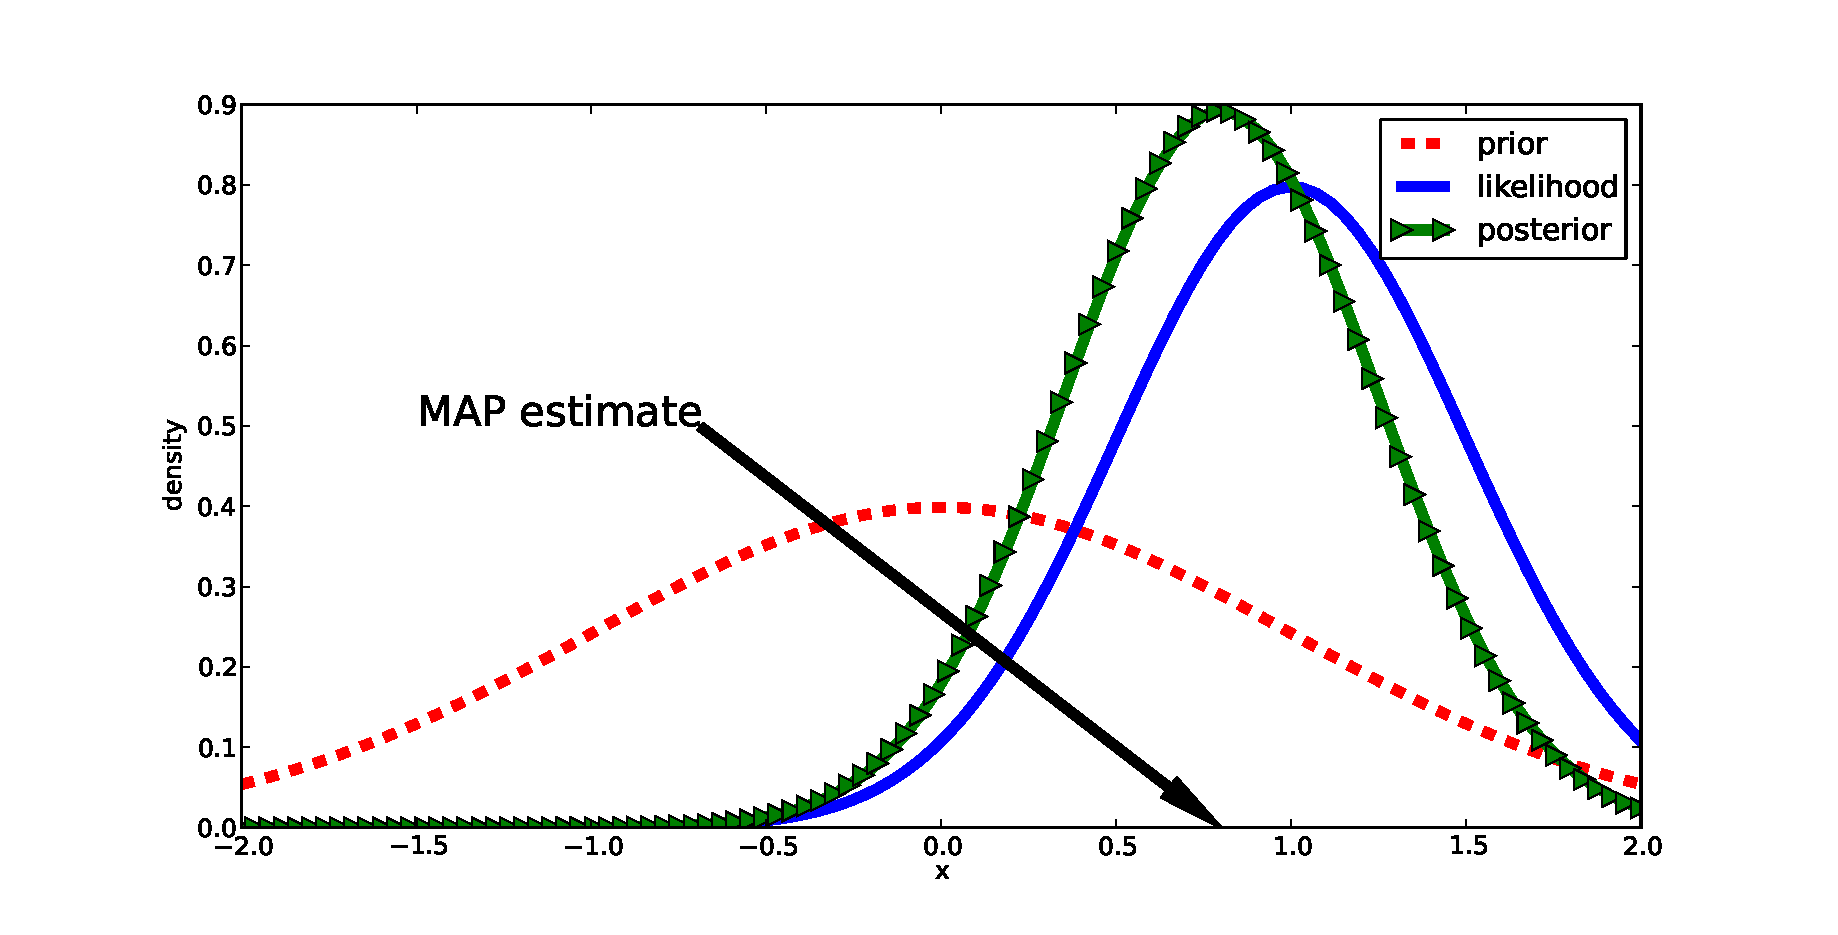
\includegraphics[width=\textwidth]{../images/gaussian-bayesian}
  \caption{The posterior is a compromise between the prior and the likelihood.}
  \label{linear:fig:gaussian-bayesian}
\end{figure}
Since the term involving $\|w\|^2$ is a sum of $K$ components, and the term involving $Y_1$ is a scalar equation, the $\|w\|^2$ term will dominate the posterior unless $w$ is small.  Therefore,  the $w$ that maximizes the posterior, $w_{map}$ will be small.  In other words, our best guess will look like a likely draw from the prior.  In this way, the posterior is a compromise between the prior and likelihood (see figure \ref{linear:fig:gaussian-bayesian}).  Specifically:
\begin{itemize}
  \item If our noise variance $\sigma_\eps^2$ was huge, then our posterior would be dominated by the prior, and our best guess $w_{map}$ would be close to zero. 
  \item If \emph{a priori} we were certain that $w_{true}$ was close to zero, then $\sigma_w$ would be small.  As a result, the $\|w\|^2$ term would be highly dominant and $w_{map}\approx0$.
  \item The likelihood slightly perturbs $w_{map}$ in a direction that fits the data.
  \item It is easy to show that the right hand side of the above minimization problem is strictly convex, so one unique solution exists.
\end{itemize}

Once we include all $N$ experiments, our posterior is
\begin{align*}
  p(w\g Y) &\propto p(Y\g w)p(w) \\
  & = p_E(Y-Xw)p(w) \\ 
  & = \exp\left\{ -\frac{1}{2\sigma_\eps^2}\|Xw-Y\|^2 \right\}\exp\left\{-\frac{1}{2\sigma_w^2}\|w\|^2\right\}.
\end{align*}
Since the product of two Gaussians is Gaussian, our posterior is Gaussian.  Our MAP solution becomes
\begin{align}
  w_{map} :&= \arg\min_w \left[  \frac{\|Xw-Y\|^2}{\sigma_\eps^2} + \frac{\|w\|^2}{\sigma_w^2}\right].
  \label{linear:align:gaussian-map}
\end{align}
Now the term $\|Xw-Y\|^2 = \sum_{n=1}^N|X_{n:}\cdot w - Y_n|^2$ is a sum of $N$ terms.  If $N\gg K$ (if we have much more data than unknowns), it will dominate and $w_{map}$ will be chosen to fit the data.

\begin{exercise}
  \label{linear:exercise:overfitting-simple}
  Show that adding more covariates to $w$ can only decrease $\|X w-Y\|$.  Does this mean that adding more covariates is always a good idea?
\end{exercise}

\begin{exercise}
  Derive \eqref{linear:align:gaussian-map}.
\end{exercise}

\begin{exercise}
  What happens to the MAP estimate as your prior uncertainty about $w$ goes to infinity (e.g. $\sigma_w\to\infty$)?  Does this seem reasonable?
\end{exercise}


The omnipotent house cat was introduced to emphasize the fact that this ideal world does not exist.  In real life, our unmodeled response $E_n$ depends on $X_{n:}$ and is certainly not Gaussian.  Furthermore, what does $w$ represent in real life?  Suppose we take the interpretation that $w$ is a vector of derivatives of the input/output response, then for what reason would our prior guess be $w\sim\calN(0, \sigma^2_wI_K)$?  All however is not lost.  If your model is not too far from reality, then your interpretation of $w$ will have meaning, and your predictions will be accurate.  This is what mathematical modeling is.  The beauty of the Bayesian approach is that it makes these assumptions explicit.  In the next section, we will see how our inevitable misspecification of error along with data quality issues will degrade our estimation/prediction, and the prior will take on the role of preventing this degradation from getting out of hand.

\section{Coefficient Estimation: Optimization Formulation}
\label{linear:section:optimization}
As we saw in section \ref{linear:section:bayesian}, in the case of Gaussian prior and error, finding the ``best guess'' coefficient $w_{map}$, is equivalent to solving the \emph{regularized least squares} optimization problem:
\begin{align}
  w_{map} :&= \arg\min_w \left\{ \|X w - Y\|^2 + \delta\|w\|^2 \right\},
  \label{linear:align:optimization}
\end{align}
with $\delta = \sigma^2_\eps/\sigma^2_w$.
In addition, solving the maximum likelihood problem gives us the classic least squares problem of finding a $w$ such that $X w$ best approximates $Y$.
\begin{align}
  w_{lq} :&= \arg\min_w \quad \|X w - Y\|^2.
  \label{linear:align:lsq}
\end{align}

% TODO Move to after remark 6.11 (after the lsq problem is solved by SVD)
\begin{exercise}
  Suppose $X\in\RNK$ and $Y\in\RN$.  In other words, suppose you take $N$ measurements and use $K$ covariates (possibly including a constant).  
  \begin{enumerate}
    \item What are the conditions on $N$ and $K$ and the rank of $X$ that ensure we have a unique solution to the unregularized least squares problem?
    \item What are the conditions on $N$ and $K$ and the rank of $X$ that ensure we have an infinite number of solutions to the unregularized least squares problem?
    \item What are the conditions on $N$ and $K$ that prevent us from having any solution to $X w=Y$ for every $Y$?
  \end{enumerate}
\end{exercise}

Solving the least squares problem can be done explicitly by multiplying both sides by $X^T$, yielding the \emph{normal equations}
\begin{align*}
  X^TXw_{ls} &= X^TY. 
\end{align*}
Assuming $X^TX$ is nonsingular, we can (in principle) invert it to find $w_{ls}$ (note that at this point we have not proved this actually finds the $w$ that minimizes \eqref{linear:align:lsq}).
\begin{align*}
  w_{ls} &= (X^TX)^{-1}X^TY,\qquad \mbox{ assuming $X^TX$ is non-singular}.
\end{align*}
Plugging $Y = Xw_{true} + E$ into this we have
\begin{align*}
  w_{ls} &= (X^TX)^{-1}X^TXw_{true} + (X^TX)^{-1}X^TE\\
  &= w_{true} + (X^TX)^{-1}X^TE ,\qquad \mbox{ assuming $X^TX$ is non-singular}.
\end{align*}
The second term is error that we hope is small.  Roughly speaking, if $X$ ``squashes'' some signals, then $(X^TX)^{-1}$ will make some noise terms ``blow up.''  The balance between how our variable selection picks out signals and how our inversion blows up noise is a delicate interplay of a special basis that we will study in the next section.


\subsection{The least squares problem and the singular value decomposition}
Here we study the singular value decomposition.  This decomposition is useful for analyzing and solving the least squares problem \eqref{linear:align:optimization}.  It is also the basis of methods such as Principle Component Analysis (PCA).  To motivate the SVD consider the lucky 
situation where your covariate matrix was diagonal, e.g.
\begin{align*}
  X &= \left( 
  \begin{matrix}
  2 & 0\\
  0 & 3
  \end{matrix}
  \right)
\end{align*}
We then have 
\begin{align*}
  Xw &= Y \Leftrightarrow \left( 
  \begin{matrix}
    2w_1\\3w_2
  \end{matrix}
  \right) = \left( 
  \begin{matrix}
    Y_1 \\ Y_2
  \end{matrix}
  \right),
\end{align*}
from which it easily follows that $w_1 = Y_1/2$, and $w_2 = Y_2/3$.  If $X$ were not diagonal but were symmetric, we could find a basis of eigenvectors $(v_1, v_2)$ such that $Xv_k = \lambda_kv_k$.  We then write $Y = (Y\cdot v_1)v_1 + (Y\cdot v_2)v_2$, and $w = \tilde w_1v_1 + \tilde w_2v_2$.  We then have $Xw=Y$ if and only if
\begin{align*}
  \lambda_1\tilde w_1v_1 + \lambda_2\tilde w_2 v_2 &= (Y\cdot v_1)v_1 + (Y\cdot v_2)v_2,
\end{align*}
which implies $\tilde w_1 = (Y\cdot v_1)/\lambda_1$ and $\tilde w_2 = (Y\cdot v_2)/\lambda_2$.  
\begin{example}
  \label{linear:example:eigendecomp}
  Consider the matrix 
  \begin{align*}
    X = \left( 
    \begin{matrix}
      2 & 1\\
      1 & 2
    \end{matrix}
    \right).
  \end{align*}
  \begin{itemize}
    \item Show that $v_1 = 2^{-1/2}(1,1)$ and $2^{-1/2}(-1,1)$ are an orthonormal basis for $\Rtwo$
    \item Show that $v_1$ and $v_2$ are eigenvectors of $X$
    \item Use that fact to find $w$ such that $Xw = (3, 4)$.
  \end{itemize}
\end{example}

An eigenvalue decomposition such as in example \ref{linear:example:eigendecomp} is possible for $X$ only if $X^TX=XX^T$.  This is never the case for non-square matrices.  Fortunately a singular value decomposition is always possible.

\begin{definition}[Singular Value Decomposition (SVD)]
  \label{linear:definition:svd}
A singular value decomposition of a matrix $X$ is a set of \emph{left singular vectors} $\left\{ u_1,\cdots,u_N \right\}$, a set of \emph{right singular vectors} $\left\{ v_1,\cdots,v_K \right\}$, and a set of \emph{singular values} $\left\{ \lambda^2_1,\cdots,\lambda^2_{N\vee K} \right\}$ ($N\vee K$ is the maximum of $N$ and $K$) such that
\begin{itemize}
  \item The $v_k$ form an orthonormal basis for $\RK$
  \item The $u_n$ form an orthonormal basis for $\RN$
  \item $Xv_j = \lambda_ju_j$, and $X^Tu_j=\lambda_jv_j$ for $j=1,\cdots,N\vee K$
  \item $\lambda_1\geq\lambda_2\geq\cdots\geq\lambda_{N\vee K}\geq0$, and if $K\leq N$, we have an $r\leq K$ such that $\lambda_{r+1}=\cdots=\lambda_N=0$.
\end{itemize}
\end{definition}
This decomposition is also sometimes written 
\begin{align}
  X &= U\Sigma V^T,
  \label{linear:align:svd}
\end{align}
where the columns of $U$ are the $u_j$, the columns of $V$ are the $v_j$, and $\Sigma\in\RNK$ has the $\lambda_j$ on its diagonal (as far as its diagonal actually goes since it is not necessarily square\ldots). 

\begin{exercise}
  Show that \eqref{linear:align:svd} follows from definition \ref{linear:definition:svd}.
\end{exercise}

\begin{exercise}
  Show that the right singular vectors (the $v_j$) are the eigenvectors of the matrix $X^TX$, and the singular values are the square roots of the eigenvalues.
  \label{linear:exercise:svd-eigen}
\end{exercise}

\begin{digression}[Simplifying Basis]
  The SVD of $X$ is a choice of basis under which the operator $X$ acts in a simple manner:  $Xv_k=\lambda_ku_k$.  This ``trick'' is widely used in mathematics.  The most famous example is probably the Fourier series.  Here, one chooses a sinusoidal basis to transform functions:
  \begin{align*}
    f(x) &= \sum_{k=1}^\infty f_k\sin2\pi kx.
  \end{align*}
  The differential operator $\d^2/\dx^2$ then takes the simple action
  \begin{align*}
    \frac{\d^2}{\dx^2}\sin2\pi kx &= -(\pi k)^2\sin2\pi kx.
  \end{align*}
  This is useful algebraically but also intuitively because nature tends to treat low and high frequencies differently (low frequency sounds travel further in water for example).  The same is true of all \emph{compact} operators (matrices being one example of this).  For that reason, we often refer to the ``tail end'' of the singular values (e.g. $\left\{ v_{N-3}, v_{N-2}, v_{N-1}, v_N \right\}$) as higher frequencies.
\end{digression}

Assuming one has an SVD of $X$ (computing that will be saved for later), we can solve the unregularized least squares problem.  Start by using the fact that the $u_n$ form an orthonormal basis to write
\begin{align*}
  Y &= \sum_{n=1}^N (u_n\cdot Y)u_n.
\end{align*}
We now seek to find a solution $w$ of the form 
\begin{align*}
  w &= \sum_{k=1}^K \tilde w_k v_k.
\end{align*}
The coefficients are written $\tilde w_k$ to emphasize that these are not the coefficients in the standard Euclidean basis.  For simplicity, let's assume a common case that $K\leq N$ and inserting the expressions for $Y$ and $w$ into $\|Xw-Y\|^2$.  This yields
\begin{align*}
  \left\|Xw - Y\right\|^2 &= \left\| X\sum_{k=1}^K\tilde w_k v_k - \sum_{n=1}^N(u_n\cdot Y)u_n\right\|^2 \\
    &\quad= \left\| \sum_{k=1}^K\tilde w_k\lambda_k u_k - \sum_{n=1}^N(u_n\cdot Y)u_n\right\|^2 \\
    &\quad= \left\| \sum_{k=1}^r(\tilde w_k\lambda_k - (u_k\cdot Y))u_k - \sum_{n=r+1}^N(u_n\cdot Y)u_n\right\|^2 \\
    &\quad= \sum_{k=1}^r \left( \tilde w_k\lambda_k - (u_k\cdot Y) \right)^2 + \sum_{n=r+1}^N(u_n\cdot Y)^2.
\end{align*}
The fourth equality follows since the $u_n$ are orthonormal.  
\begin{remark}
  \label{linear:remark:svd-soln}
We note a few things:
\begin{itemize}
  \item If $N>K$, there is an exact solution to $Xw=Y$ if and only if $u_n\cdot Y=0$ for $n>r$.
  \item Solutions to the unregularized least squares problem \eqref{linear:align:lsq} are given by:
    \begin{align*}
      \tilde w_k &= \left\{ 
        \begin{matrix}
          &(u_k\cdot Y)/\lambda_k,\quad 1\leq k\leq r\\
          &\mbox{anything},\quad r+1\leq k\leq K.
        \end{matrix}
      \right\}
    \end{align*}
  \item Setting $\tilde w_k\equiv0$ for $k>r$ gives us the so-called \emph{minimal norm solution}.
    \begin{align*}
      \arg\min\left\{ \|\hat w\|^2\st \hat w \mbox{ is a solution to \eqref{linear:align:lsq}}\right\}.
    \end{align*}
  \item The (Moore-Penrose) \emph{pseudoinverse} $X^\dagger$ is defined by
    \begin{align*}
      X^\dagger Y &= \sum_{k=1}^r \frac{u_k\cdot Y}{\lambda_k}v_k.
    \end{align*}
    In other words, $X^\dagger Y$ is the minimal norm solution to the least squares problem.  One could just as easily truncate this sum at $m\leq r$, giving rise to $X^{\dagger,m}$.
\end{itemize}
\end{remark}

There exist a variety of numerical solvers for this problem.  So long as the number of covariates $K$ is small, most will converge on (approximately) the solution given above.  The $1/\lambda_k$ factor however can cause a huge problem as we will now explain.  Recall that our original model was:
\begin{align*}
  Y &= Xw_{true} + E = \sum_{k=1}^K (w_{true}\cdot v_k)\lambda_k u_k + \sum_{n=1}^N(E\cdot u_n)u_n.
\end{align*}
Inserting this into the expression $\tilde w_j = (u_j\cdot Y)/\lambda_j$, we have
\begin{align}
  \begin{split}
    \tilde w_j &= w_{true}\cdot v_j + \frac{E\cdot u_j}{\lambda_j}
    = \frac{\lambda_j(w_{true}\cdot v_j) + E\cdot u_j}{\lambda_j}
    = \frac{\left[ Xw_{true} + E \right]\cdot u_j}{\lambda_j}.
  \end{split}
  \label{linear:align:coefficient-with-error}
\end{align}

The term $Xw_{true}\cdot u_j$ is our modeled output in direction $u_j$.  Similarly, $E\cdot u_j$ is a measure of the unmodeled output in direction $u_j$.  If our unmodeled output in this direction is significant, our modeling coefficient $\tilde w_j$ will differ from the ``true'' value.  Moreover, as $\|Xv_j\| = \|\lambda_ju_j\| = \lambda_j$, the singular value $\lambda_j$ can be seen as the magnitude of our covariates pointing in direction $v_j$.  If our covariates did not have significant power in this direction, the error in $\tilde w_j$ will be amplified.  Thus, the goal for statistical inference of coefficients is clear:  Either avoid this ``large error'' scenario (by modeling better and avoiding directions in which your data is sparse) or give up on modeling these particular coefficients accurately.  For prediction the situation isn't so clear.  Suppose we have a new input $x$.  Our ``best guess'' output is 
\begin{align}
  \begin{split}
    \hat y = x\cdot \tilde w & = \left( \sum_{k=1}^K(x\cdot v_k)v_k \right)\cdot \left( \sum_{k=1}^K \left[ \frac{\left[ Xw_{true} + E \right]\cdot u_k}{\lambda_k} \right]v_k\right) \\
    &= \sum_{k=1}^K(x\cdot v_k)\left[ \frac{ \left[ Xw_{true} + E \right]\cdot u_k}{\lambda_k} \right].
  \end{split}
  \label{linear:align:fundamental}
\end{align}
Assume we are in the ``large error'' scenario as above.  Then the term in square brackets will be large.  If however the new input $x$ is similar to our old input, then $x\cdot v_j$ will be small (on the order of $\lambda_j$) and the error in the $j^{th}$ term of our prediction will be small.  In other words, if your future input looks like your training input, you will be ok.

\begin{exercise}
  Assume we measure data but one variable is always exactly the same as the other.  What does this imply about the rank of the variable matrix $X$?  Show that this means we will have at least one singular value $\lambda_k=0$ for $k\leq K$.  Since singular values change continuously with matrix coefficients, this means that if two columns are almost the same then we will have a singular value $\lambda_k\ll1$.  This is actually more dangerous since if $\lambda_k=0$ your solver will either raise an exception or not invert in that direction, but if $\lambda_k\ll1$ most solvers will go ahead and find a (noisy) solution.
\end{exercise}

\begin{exercise}
  Using \eqref{linear:align:coefficient-with-error} show that if $X$ and $E$ are independent, then $\Exp{w} = w_{true}$.

  Note that since $\lambda_j\sim O(N)$ and in the uncorrelated case $E\cdot u_j\sim O(\sqrt{N})$, one can show that if the errors are uncorrelated with the covariates then $w\to w_{true}$ as $N\to\infty$.
\end{exercise}

\subsection{Overfitting examples}
The next exercise and example are instances of \emph{overfitting}.  Overfitting is a general term describing the situation when the noise term in our training data $E$ has too big an influence on our model's fit.  In this case, our model will often fit our training data well, but will not perform well on future data.  The reason is that we have little understanding of the noise term $E$ and very little understanding of what it will do in the future.  

\begin{example}
The most classic example is that of polynomial fitting.  Suppose our actual data is generated by
\begin{align}
  y = x + x^2 + x^3 + \eps(x), \quad x=0, 0.1,\cdots,1.0.
  \label{linear:align:poly}
\end{align}
We fit this data by minimizing the mean square error of both three and six degree polynomials (equivalently maximizing the obvious likelihood function).  This can be done with the following Python code.

\rule{\textwidth}{2pt}
\begin{minted}{python}
import scipy as sp
import matplotlib.pyplot as plt 

x = sp.linspace(0, 1, 10) 
x_long = sp.linspace(-0.1, 1.1, 100)

y = x + x**2 - x**3 + 0.1 * sp.randn(len(x))

z = sp.polyfit(x, y, 3)
p = sp.poly1d(z)
print "3-degree coefficients = %s" % z 

z6 = sp.polyfit(x, y, 6)
p6 = sp.poly1d(z6)
print "6-degree coefficients = %s" % z6

plt.clf()
plt.plot(x, y, 'b.', ms=18, label='Y')
plt.plot(x_long, p(x_long), 'r-', lw=5, label='3-degree poly')
plt.plot(x_long, p6(x_long), 'g--', lw=6, label='6-degree poly')
plt.xlabel('X')
plt.legend(loc='best')

plt.show()
\end{minted}
\rule{\textwidth}{2pt}

See figure \ref{linear:figure:polyfit}.
\begin{figure}
  \label{linear:figure:polyfit}
  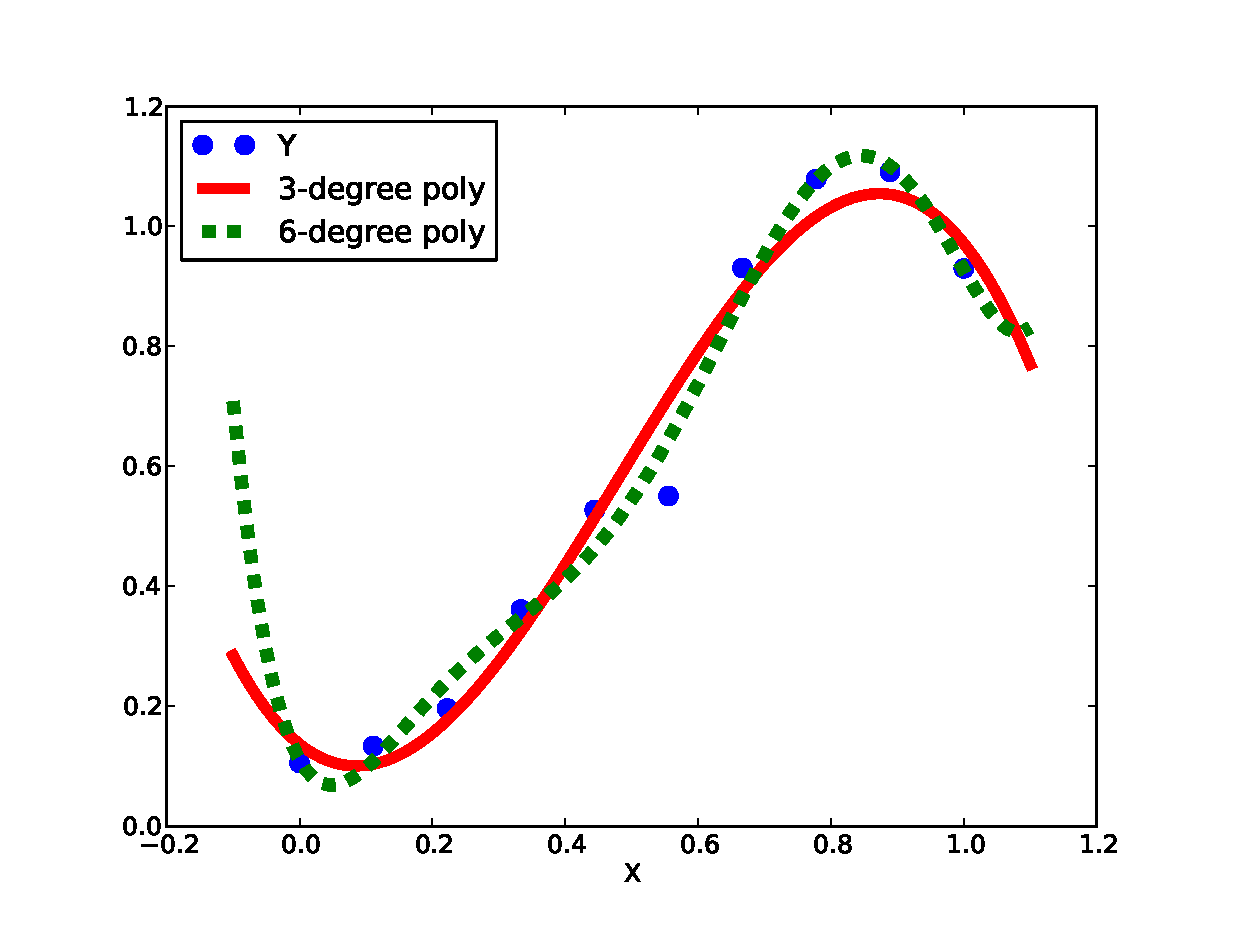
\includegraphics[width=0.7\textwidth]{../images/polynomial}
  \caption{Polynomial fitting and overfitting}
\end{figure}
The third degree polynomial fits well but not perfectly at every point.  The six degree polynomial fits the data better, but wiggles in a ``crazy'' manner, and looks like it will ``blow up'' outside the range of $[0,1]$.  Furthermore, running this code multiple times shows that all coefficients in the six degree polynomial are highly dependent on the error and the first three terms are no where near the real terms.  For statistical inference this is a killer:  How can you report these coefficients as ``findings'' when they so obviously depend on the unmodeled noise?  For prediction the situation is slightly more nuanced.  If we believe future $x$ values will fall outside the interval $[0,1]$, then we are clearly in trouble.  On the other hand, if future values lie inside this interval then it can be seen that our polynomial, no matter how crazy it is, will predict quite well.  Beware however:  In higher dimensions it becomes difficult to determine the range of applicability of your model.  It is usually better to be safe and error on the side of underfitting.  Note that this is an example of the more general result of equation \eqref{linear:align:fundamental}.
\end{example}


\begin{exercise}[Misspecification of error correlations]
  Let's model percentage stock returns among four different stocks (the relative percentage change in stock price over one day).  We will model the tomorrows returns as depending on todays returns via the relation $y = w_1x + w_2x^2 + \eps$, where $\eps$ is uncorrelated for every stock (recall that ordinary least squares implicitly makes this assumption).  Let's assume the real life model is $y = x + 0.05x^2 + \eta$, where $\eta$ for different stocks is sometimes uncorrelated and sometimes correlated. Since, on most days, returns are around $\pm1\%$, we have approximately a 10 to 1 signal to noise ratio and think that we're ok.  Taking measurements of the stock prices on one day we get our data matrix (first column is the returns, second column is the squared returns).
  \begin{align}
    X &= \left( 
    \begin{matrix}
      1 & 1\\
      -1 & 1 \\
      1 & 1 \\
      -1 & 1
    \end{matrix}
    \right).
    \label{linear:align:bad-matrix}
  \end{align}
  \begin{enumerate}
    \item Use exercise \ref{linear:exercise:svd-eigen} to show that the right singular vectors are $v_1=(1,0)^T$, and $v_2=(0,1)^T$, and the singular values are $\lambda_1=\lambda_2=2$.
    \item Use the fact that $Xv_j = \lambda_ju_j$ to show that $u_1=0.5\cdot(1, -1, 1, -1)^T$, and $u_2=0.5\cdot(1, 1, 1, 1)^T$.
    \item Suppose we measured returns the day after and got $Y = (1.25, -1.15, 0.85, -0.75)^T$.  One could use $y = x + 0.05x^2 + \eta$ to explicitly calculate $\eta$ and infer that the noise was basically uncorrelated (all 4 $\eta$ were not related).  Use remark \ref{linear:remark:svd-soln} to show that our estimate for $w$ is $(1, 0.05)$, which is the exact result in the uncorrelated model.  Note:  Since $(v_1, v_2)$ are the standard basis, the coefficients for $w$ estimated by \ref{linear:remark:svd-soln} will be in the standard basis as well.
\item Suppose instead that we measured $\tilde Y=(1.15, -0.85, 1.15, -0.85)$.  So the noise was correlated.  Show that our estimate is $w = (1, 0.15)$.  The coefficient for $w_2$ was three times larger than before!
\item What will happen if we use the second coefficient to predict returns during uncorrelated times?  What about during times when the error is negative and correlated?   What about positive and correlated?
  \end{enumerate}
  Note that if errors were always correlated, say with correlation matrix $\Sigma$, one should solve the generalized least squares problem:
  \begin{align*}
    \hat w &= \arg\min_w (Xw - Y)^T\Sigma^{-1}(Xw-Y).
  \end{align*}
  This can be seen by reworking the example in section \ref{linear:subsection:gaussian-example}, starting with the assumption $E\sim\calN(0, \Sigma)$.

  One could also take the viewpoint that while we cannot hope to specify the error model correctly, we do know \emph{a priori} that the coefficient of $x^2$ should be smaller than that of $x$.  In this case, we could use a prior proportional to 
  \begin{align*}
    \exp\left\{ -\frac{1}{2}\left[ \frac{w_1^2}{2\lambda_w^2} + \frac{w_2^2}{2\cdot0.1\cdot\lambda_w^2} \right] \right\}.
  \end{align*}
  Alternatively, we could fit our model to fake data that was perturbed by different noise models.  If the results show wild swings in the coefficients then we should be cautious.
\end{exercise}

\begin{example}
  \label{linear:example:small-singular-values}
Another example starts with the data matrix
\begin{align*}
  X &= 
  \left( 
  \begin{matrix}
    1 & 1.01\\
    1 & 1
  \end{matrix}
  \right).
\end{align*}
This matrix is almost singular because the two rows are almost the same.  This happened because, over our measured data set, the two covariates were almost the same.  If our model is good, we expect the two measured responses $Y_1$, $Y_2$ to be almost the same (either that or we have some pathological case such as $y = 1000(x_1 - x_2)$).  One finds that the singular values are $\lambda_1=2.005$, $\lambda_2=0.005$.  The smaller singular value is a problem.  It is associated with the singular directions $v_2=(0.71, -0.71)$, $u_2=(-0.71, 0.71)$.  This means that 
\begin{align*}
  0.71(w_1 -w_2) = \tilde w_2 &= 200\cdot0.71(Y_2 - Y_1).
\end{align*}
In other words, our coefficient is extremely sensitive to $Y_1-Y_2$.  Small differences between the two will lead to a huge difference in $w$ (note that this will not lead to huge changes in $w_1+w_2$, only $w_1-w_2)$.  The upshot is that our predictive model will work fine so long as future $x$ values have $x_1\approx x_2$ (just like our training data), but if we stray outside the range of our training data we are in for big problems.
\end{example}

\subsection{$L_2$ regularization}
As was mentioned earlier, the Bayesian MAP problem reduces, in the Gaussian case, to the optimization problem
\begin{align}
  w_\delta :&= \arg\min_w \left\{ \|Xw - Y\|^2 + \delta\|w\|^2 \right\}.
  \label{linear:align:regularized-lsq}
\end{align}
With ``no math'' whatsoever, one can see that the \emph{penalty term} $\|w\|^2$ acts to prevent $w$ from becoming too big.  As with classical least squares, the SVD provides insight into exactly what is happening.

\begin{theorem}
  If $\delta>0$ then the solution to \eqref{linear:align:regularized-lsq} exists, is unique, and is given by the formula
  \begin{align*}
    w_\delta &= (X^TX + \delta I)^{-1} X^TY = \sum_{k=1}^K \frac{\lambda_k}{\lambda_k^2 + \delta}(Y\cdot u_k)v_k
  \end{align*}
  \label{linear:theorem:regularized-lsq}
\end{theorem}
\begin{proof}
  The second equality follows from definition \ref{linear:definition:svd} and exercise \ref{linear:exercise:svd-eigen}.  To show the first equality let $F(w):= \|X w-Y\|^2 = \delta\|w\|^2$.  We then have, for any vector $z$,
  \begin{align*}
    F(w_\delta+z) &= F(w_\delta) + 2z^T\left( (X^TX + \delta I)w_\delta - X^TY \right) + \|X z\|^2 + \delta\|z\|^2 \\
    &= F(w_\delta) + \|X z\|^2 + \delta\|z\|^2.
  \end{align*}
  Since the second term vanishes only when $z=0$, we see that $F(w_\delta+z)$ is minimized when $z=0$.  Thus $w_\delta$ minimizes $F$ and we are done.
\end{proof}

\begin{remark}
  As $\delta\to0$ it is easy to see that the regularized solution converges to the minimal norm solution.  For $\delta>0$ the solution components associated with the smaller singular values are attenuated more.  This is fortunate since these components can be quite troublesome as example \ref{linear:example:small-singular-values} has shown.  
\end{remark}

\subsection{Choosing the regularization parameter}
\label{linear:subsection:cross-validation}
Much has been written on techniques (Bayesian or otherwise) to choose optimal regularization parameters.  These (asymptotic) optimality results usually rely on assumptions about the error model (i.e. that your error model is correct or ever that the error is uncorrelated to the covariates).  This is unfortunate since this is usually not the case.  There is also the method of \emph{hierarchical Bayesian} modeling.  Here, the prior is left unspecified and the data determines it.  While accepting that these results do have their place we prefer instead to show the simple method of \emph{cross validation}.  

A typical cross validation cycle would go as follows:
\begin{enumerate}
  \item Choose a number of possible values for $\delta$, call them $(\delta_1,\cdots,\delta_M)$.  For every $\delta_m$\ldots
  \item Segregate your observations into a \emph{training set} $X^{train}$, $Y^{train}$ and a \emph{cross validation set} $X^{cv}$, $Y^{cv}$.  A common split would be 70-30.
  \item For every $\delta_m$, use the training data to solve the regularized least squares problem \eqref{linear:align:regularized-lsq} obtaining $(w_{\delta_1},\cdots,w_{\delta_M})$.
  \item For every $m$, measure the \emph{cross validation error} (here it is a relative root-mean-square error) $\|X^{cv}w_{\delta_m} - Y^{cv}\|/\|Y^{cv}\|$.
  \item Choose $\delta$ to be the $\delta_m$ that minimizes that error.
  \item Train your model using the full data set and $\delta$ from above.
\end{enumerate}

Step 1 chooses a bigger set of data for training than cross validation.  This is typical because you are training $K$ different parameters, but (in this case) only using cross validation to find one.  Thus, we are not worried so much about overfitting a small data set.  The $\delta_m$ in step 2 are usually picked by first guessing a few values of $\delta$ and seeing over what range of values the training data misfit isn't too horrible.  In step 3 we solve the regularized problem multiple times.  Note that if we were to measure the training data (unregularized) least squares error $\|X^{train}w_{\delta_m}- Y^{train}\|/\|Y^{train}\|$ we would see the training error get worse monotonically as $\delta$ increases.  What we care about (and measure in step 4) is the cross validation set error.  The hope is that the error $\eps^{cr}$ will be such that problems associated with overfitting show up here.  Note that there is nothing canonical about the choice of error in step 4.  If for example you care more about large errors, a fourth order error function could be used.  In step 5 we choose $\delta$ as the minimizer of the cross validation error.  Again, different choices could be made.  For example, one may have generated the training and cross validation sets by sampling people in 2010.  It may or may not be reasonable to believe people in 2013 will act according to the same model.  If they don't the error function $\eps(x,z)$ could be much different and this could cause your model to behave poorly when fed with 2013 data.

\begin{exercise}
  Use the SVD to show that the mean square training error gets worse monotonically with increasing $\delta$.
\end{exercise}

Unlike the training (mean square) error, the cross validation error does not always change monotonically.  If for example, the variable matrix $X$ had highly correlated columns, then the singular values will rapidly decrease.  This in turn causes an overfitting effect.  In our idealized $Y = Xw + E$ world this means that $\hat w$ will be far from $w_{true}$.  As a result, the cross validation error will (on average) be convex (see figure \ref{linear:fig:overfitting} left).  If on the other hand your variables were uncorrelated, then there is no reason to believe that the model will overfit to the noise, and it is possible that both training and cross validation error will monotonically increase (see figure \ref{linear:fig:overfitting} right).  The reader is cautioned however that in the ``real world'' the data is not generated by $Y = Xw + E$ with uncorrelated $E$, and more complex behaviors can emerge.  In particular, the modeler may intend on using the model on real-world inputs that behave differently than the training (or cross-validation) input.  For example, both the training and cross validation data could be from pre 2008 (before the financial crisis) but you will use your model in a post 2012 world.  These \emph{out of time} errors can be especially problematic.  In this case, the modeler can error on the side of caution and use more regularization than the cross-validation cycle above suggests.  Another popular method is to reduce the number of variables to a smaller set that is human interpretable (e.g., a human can check that the coefficient in front of a particular variable is reasonable).

\begin{figure}
  \label{linear:fig:overfitting}
  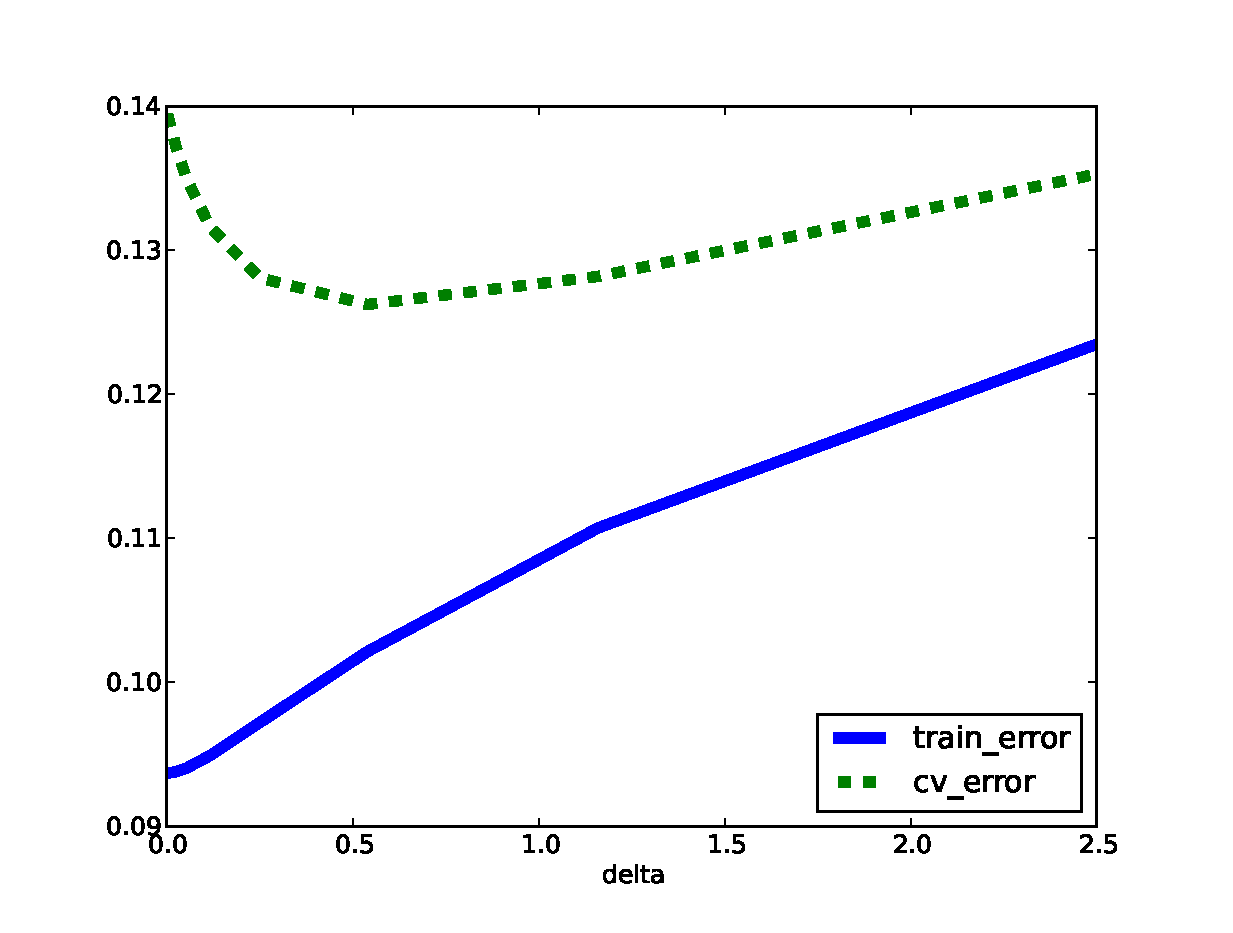
\includegraphics[width=0.5\textwidth]{../images/train-cv-error}
  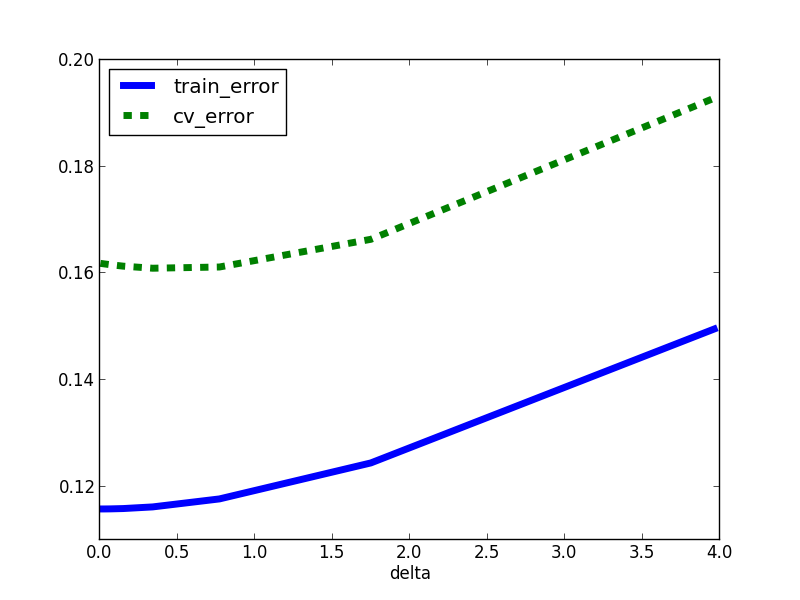
\includegraphics[width=0.5\textwidth]{../images/train-cv-error2}
  \caption{Cross validation and test errors.  Left:  The $X$ matrix with correlated columns, hence the unregularized solution was overfitting.  Right:  The $X$ matrix had uncorrelated columns and therefore the unregularized solution was not overfitting.}
\end{figure}

\subsection{Numerical techniques}
\label{linear:subsection:numerical}
The conclusion of theorem \ref{linear:theorem:regularized-lsq} implies that one can find $w_\delta$ by solving:
\begin{align}
  (X^TX + \delta I)w_\delta &= X^TY.
  \label{linear:align:reg-problem}
\end{align}
It is easy to show that the condition number of $A:=(X^TX + \delta I)$ is at least as large as $\delta$.  So when $\delta>0$ is large enough the problem is well-posed and can be solved directly even for large $N, K$ (e.g. $N=K=1000$ gives little trouble).  If $\delta=0$ and columns of $X$ are linearly dependent, you will not be able to invert $X^TX$.   Even if $X^TX$ is invertible in theory, if $\delta$ is small then numerical error can cause error (e.g. when the condition number is in the millions).

Alternatively, one can compute the SVD of $X$ and then use the pseudoinverse $X^\dagger$.  This has the advantage of not having to worry about linearly dependent columns (sometimes however is is often nice to know that your columns are dependent).  Moreover, computing the SVD of $X$ can be done in a stable manner even for large matrices.

The ``best'' alternative for small or medium matrices is to factor the matrix into a simpler form.  One example is the $QR$ factorization.  We write $X^TX = QR$ with $Q$ orthogonal and $R$ upper triangular.  The resultant normal equations ($QRw = X^TY$) are then trivial to solve.  First we multiply by $Q^T$ (which is $Q^{-1}$), then solve the system of equations $Rw = Q^TX^TY$ (which is trivial since $R$ is triangular).  This has the advantage of being numerically very stable and quicker than the SVD.  

The methods described so far are not suited for larger problems because they require the full matrix to exist in memory, and attempt to completely solve the problem (which is difficult and unnecessary for large problems).  In this case, an iterative technique is used.  Here we start with a guess $w^0$, and iteratively improve it until we have reduced the \emph{residual} $\|Xw^\ell - Y\|$ to a small enough value.  These iterative techniques typically require evaluation of $Xu$ for various vectors $u$.  This does not require storing $X$ (you only need to stream $X$ in and out of memory, and multiply things while things are in memory).  For the case of a large sparse (most entries are zero) you can store the nonzero values and use these to perform multiplication.  Moreover, rather than completely solving the problem, you can stop at any point and obtain an approximate solution.


\section{Variable Scaling and Transformations}
To motivate this section, consider the linear model $y = w_1 + w_2x +\eps$, where $y$ is ``wealth'', and $x$ is a person's height.  If height is measured in millimeters, then $x$ will be around 1,500.  If on the other hand height is measured in meters, then $x$ will be around 1.5.  Intuition tells us that when height is measured in millimeters (and thus $x$ is very large), the optimal $w_1$ will be much smaller.  This is a form of prior belief.  This section will conclude:
\begin{enumerate}
  \item Maximum likelihood estimation require no special attention to variable scale (except for possible numerical issues) to produce optimal coefficients.
  \item Bayesian estimates will be flawed unless the prior is adjusted in accordance with variable scale (or the variables all have the same scale).
  \item In all cases, scaled variables are often easier to interpret.
\end{enumerate}
\subsection{Simple variable scaling}
Returning to our height example, suppose we use millimeters and find an optimum $w_{ml}$ using least squares.  In other words, 
\begin{align*}
  w_{ml} &= \arg\min_w \sum_{n=1}^N \left( w_0 + w_1 X_{n1} - Y_n \right)^2.
\end{align*}
Suppose we change to meters.  Then the heights, $X_{n1}$, change to $\tilde X_{n1} = X_{n1}/1000$.  We then seek to find $\tilde w_{ml}$, the maximum likelihood solution in these new variables.  Rather than re-solving the problem, we can write the above equation as
\begin{align*}
  w_{ml} &= \arg\min_w \sum_{n=1}^N \left( w_0 + w_1\cdot1000 \cdot\frac{X_{n1}}{1000} - Y_n \right)^2 \\
  &= \arg\min_w \sum_{n=1}^N \left( w_0 + w_1\cdot1000 \cdot\tilde X_{n1} - Y_n \right)^2.
\end{align*}
Since $w_{ml}= ( (w_{ml})_0, (w_{ml})_1)$ minimizes the above sum, we see that the minimizing multiplier of heights (in meters) is $w_1\cdot1000$.  Therefore, $\tilde w_{ml} = ( (w_{ml})_0, 1000\cdot(w_{ml})_1)$.  In other words, when the variable $x$ got 1000 times smaller, its coefficient got 1000 times larger.  In either case, solving a simple least squares problem should produce the correct answer.  In both cases, the residual error $\|Xw_{ml}-Y\|^2$ will be the same. 

Although we are in theory able to ignore variable scaling, practical matters make us reconsider.  Recalling our discussion in previous sections, we would like to use huge variables as an common symptom of overfitting. Note however that in one case the second component of $w_{ml}$ is 1000 times larger than the other case.  So we obviously cannot look at raw coefficient magnitude as a symptom of overfitting.  Moreover, the normal matrix $X^TX$ will have bottom right entry equal to $\sum_n X_{n1}^2$, which could be huge if we are using millimeters.  Many linear algebra packages would have trouble solving maximum likelihood problem.  In other cases this sum could be so large or small that our computer cannot store it.  Suppose further that we used both \emph{height} and \emph{health} as variables.  Then, our choice of units to represent height/health in would influence the absolute values of our coefficients.  We would not be able to say, ``the coefficient of height is 10 times larger, and therefore height is probably more important.''  Although this is not the proper way to conclusively judge variable importance, it is a good way to get rough guesses that can be used to find model issues (e.g. if the coefficient of health was almost zero, we should be surprised).

The most common solution to this issue is to rescale columns of $X$ by the sample standard deviation of the columns.  In other words, with 
\begin{align*}
  \mu_k :&= \frac{1}{N}\sum_{n=1}^N X_{nk},\qquad \sigma_k := \sqrt{\frac{1}{N-1}\sum_{n=1}^N \left( X_{nk} - \mu_k \right)^2}.
\end{align*}
we replace the column $X_{:k}$ with $X_{:k}/\sigma_k$.  In addition to scaling by $\sigma_k^{-1}$, it is common to subtract the mean, leading to
\begin{definition}[Variable standardization]
  \label{linear:definition:standardization}
  Assume we augment our data matrix $X$ with a constant zeroth column $X_{:0}\equiv1$.  \emph{Variable standardization} is the process of replacing $X$ with $\hat X$, where
  \begin{align*}
    \hat X_{:0} &= X_{:0} \equiv 1,\qquad \hat X_{:k} = (X_{:k} - \mu_k) / \sigma_k,\quad k=1,\cdots,K.
  \end{align*}
  Solving the ML (maximum likelihood) problem with $\hat X$ gives us the coefficients $\hat w$.  They are related to the standard ML coefficients by
  \begin{align*}
    w_0 &= \hat w_0 - \sum_{k=1}^K\frac{\mu_k\hat w_k}{\sigma_k},\qquad w_k = \frac{\hat w_k}{\sigma_k},\quad k = 1,\cdots,K.
  \end{align*}
\end{definition}

A typical workflow involves first standardizing the data (converting $X$ to $\hat X$), then fitting the coefficients $\hat w$.  Second, we inspect the coefficients $\hat w$, looking for irregularities, and re-compute if necessary.  If we intend on predicting a new output $y$ given a new input $x$, we could either standardize $x$ (using the \emph{exact same} $\mu_k$, $\sigma_k$ as above), or we could translate $\hat w$ into $w$ and use the un-standardized $x$ with $w$.  

\begin{exercise}
  For the standardized coefficients of definition \ref{linear:definition:standardization} show that:
  \begin{enumerate}
    \item The constant coefficient $\hat w_0$ is equal to the predicted output $y$ when the input vector $x$ is equal to its mean.
    \item The coefficient of $\hat X_{:k}$ defined above does not change when the units used to measure $X_{:k}$ change.
    \item The translation $\hat w\mapsto w$ is as given above.
  \end{enumerate}
\end{exercise}

Moving on to Bayesian MAP estimates, let's revisit the ``happiness as a function of height'' problem.  Now we have
\begin{align}
  w_\delta &= \arg\min_w \left[ \sum_{n=1}^N \left( w_0 + w_1 X_{n1} - Y_n \right)^2 + \delta (w_0^2 + w_1^2)\right].
  \label{linear:align:millimeter-map}
\end{align}
Suppose we measure height in meters and find $w_\delta$.  In this case, $X_{n1}$ is around 1.  Suppose we find that the ML $w_1$ is approximately equal to one.  If on the other hand we use millimeters, then the ML $w_1$ will be 1,000 times smaller, and if we do not adjust $\delta$ the penalty term $\delta w_1^2$ will have little influence on the MAP solution.  We could adjust $\delta$ (making it 1,000 times larger), but then the other penalty term $\delta w_0^2$ would be huge.  As a result, if we change our unit of measurement to millimeters then our model will have no constant!  The problem is that we have used the same prior in both cases.  Recall that \eqref{linear:align:millimeter-map} is the result of the prior $w_k\sim\calN(0, 2/\delta)$, for $k=0,1$.  However, if we are using millimeters, then we expect $w_1$ to be 1,000 times smaller than before, which means we should change $\delta\mapsto\delta/1000^2$.

Consider the more general MAP problem with a data matrix $X$ (with a constant column $X_{:0}$ prepended).
\begin{align*}
  w_\delta :&= \arg\min_w \left[ \|Xw-Y\|^2 + \delta\|w\|^2 \right].
\end{align*}
As above, the optimal $w_\delta$ will depend strongly on the unit of measurement used for the columns of $X$.  To correct for this, we could use a different prior for each column.  The prior variance should be inversely proportional to the scale of the variable.  One way to achieve this is to let $\delta$ be a vector where $\delta_k\propto1/\sigma_k$ (for $k=1,\cdots,K$).  Similar (but not identical) ends can be obtained however by first standardizing $X$ and then using the same $\delta$ for all variables $w_k$, $k=1,2,\cdots,K$.  Typically the constant is not regularized.  The resultant MAP problem is to find
\begin{align}
  \hat w(\delta) :&= \arg\min_{\hat w} \left[ \|\hat X\hat w - Y\|^2 + \delta \sum_{k=1}^K\hat w_k^2 \right].
  \label{linear:align:standardized-map}
\end{align}
The Bayesian interpretation of \eqref{linear:align:standardized-map} is that we believe \emph{a-priori} that each coefficient $\hat w(\delta)_k$, $k=1,\cdots,K$ will have approximately the same magnitude, and that the magnitude of $w_0$ could be much bigger.  The choice to not regularize (or to weakly regularize) the constant can be justified by noting that if the un-modeled output $\eps$ contained a constant term, then we would likely be better off including this term in our model.  Not regularizing the constant allows the constant to vary as much as possible to fit capture the constant part of the ``noise.''  The non-constant part of the noise will not affect the coefficient $w_0$ much at all since constants project strongly only on the first few singular vectors (details are left to the reader).


\subsection{Linear transformations of variables}
In general, one can change basis in each sample $X_{n:}$ to the columns of the $K\times K$ invertible matrix $A$, giving $A^TX_{n:}$.  This leads to get a new variable matrix $(A^TX^T)^T = XA$.  Let us set
\begin{align*}
  w^A(\delta) &= \arg\min_w \left[ \|XA w - Y\|^2 + \delta\|w\|^2 \right].
\end{align*}
Theorem \ref{linear:theorem:regularized-lsq} shows that
\begin{align*}
  w^A(\delta) &= (A^TX^TXA + \delta I)^{-1}A^TX^TY.
\end{align*}
Setting $\delta$ to zero, we see that $w^A(0) = A^{-1}(X^TX)^{-1}X^TY = A^{-1}w_{ml}$.

\begin{exercise}
  With $v_1,\cdots,v_K$ and $\lambda_1,\cdots,\lambda_K$ the right singular vectors and first $K$ singular values of $X$, set $A = VC$ where the columns of $V$ are the $v_k$ and
  \begin{align*}
    C = \left( 
    \begin{matrix}
      \lambda_1^{-1} & 0 & \cdots & 0\\
      0 &\lambda_2^{-1} & \cdots & 0\\
      \vdots & \vdots & \ddots \\
      0 & 0 & \cdots & \lambda_K^{-1}
    \end{matrix}
    \right).
  \end{align*}
  \begin{enumerate}
    \item Show that, the new variables $\tilde X := XA$ satisfy $\tilde X^T\tilde X = I$.  For this reason, $A$ is called a \emph{whitening} matrix.
    \item Show that 
      \begin{align*}
        w^A(0) &= (Y\cdot u_1,\cdots,Y\cdot u_k).
      \end{align*}
      Since we are not dividing by $\lambda_k$ it appears the problem is robust to noise.
    \item Use the relation $w_{ml} = Aw^A(0)$ to show that
      \begin{align*}
        w_{ml} &= \sum_{k=1}^K \frac{Y\cdot u_k}{\lambda_k}v_k,
      \end{align*}
      as always.  So if we have small $\lambda_k$ the problem is not robust to noise??!?!?!?!?!  
  \end{enumerate}
\end{exercise}
  The above exercise shows that the robustness of your coefficients to noise is highly dependent on the variable representation you choose.  Some linear combinations of coefficients will be robust, and others won't.  At the end of the day however, your predictive model $Xw$ is unchanged by a change of basis in the ML formulation.  The Bayesian MAP solution is a different story.  The best advice to give is to choose your prior wisely.

\subsection{Nonlinear transformations and segmentation}
Suppose we try to model height as function of age.  From birth to 17 years of age we would see fairly steady increase in mean height.  After that, mean height would level out until during old age it would decrease.  
\begin{figure}
  \label{linear:fig:mean-height}
  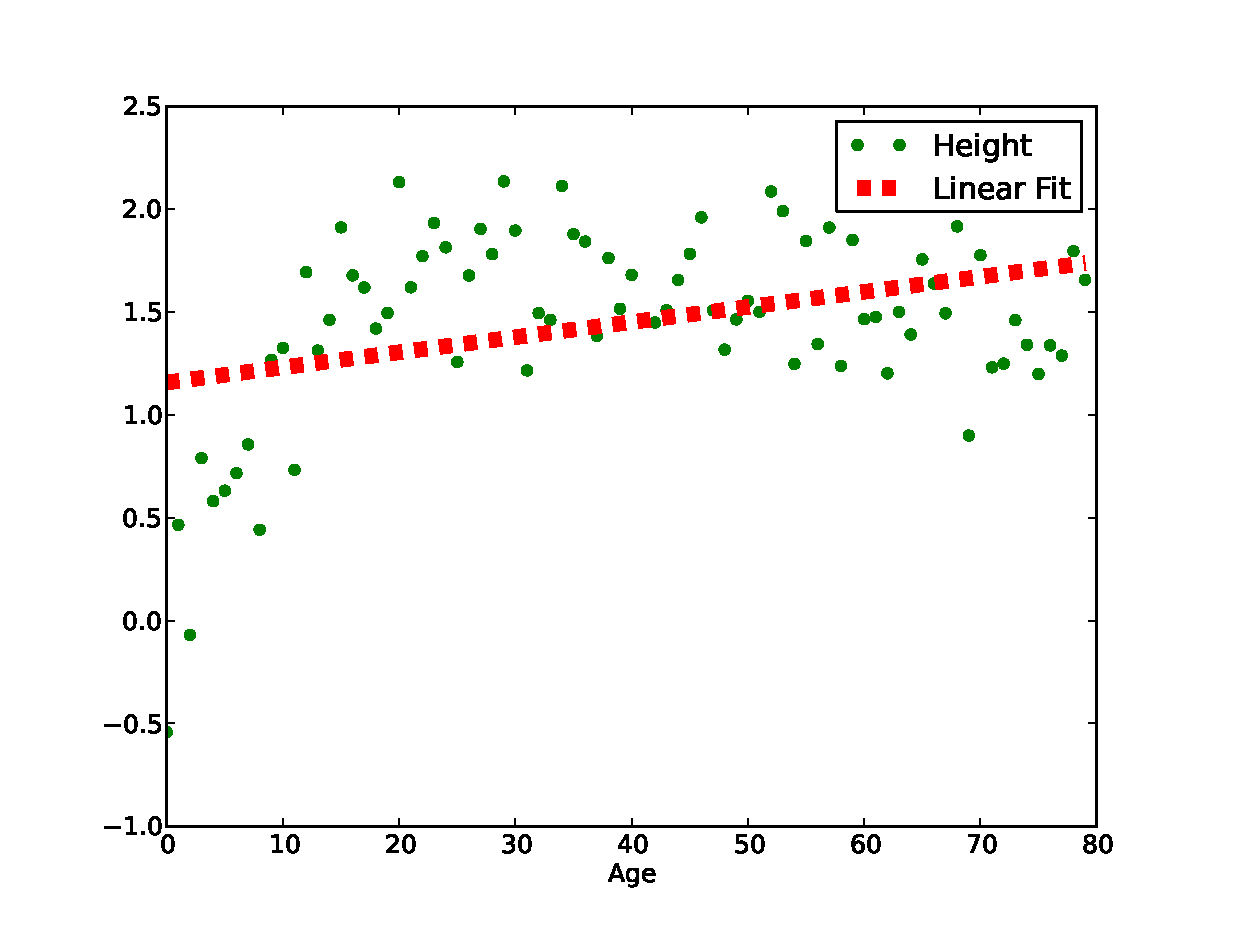
\includegraphics[width=0.5\textwidth]{../images/height_v_age_linearfit}
  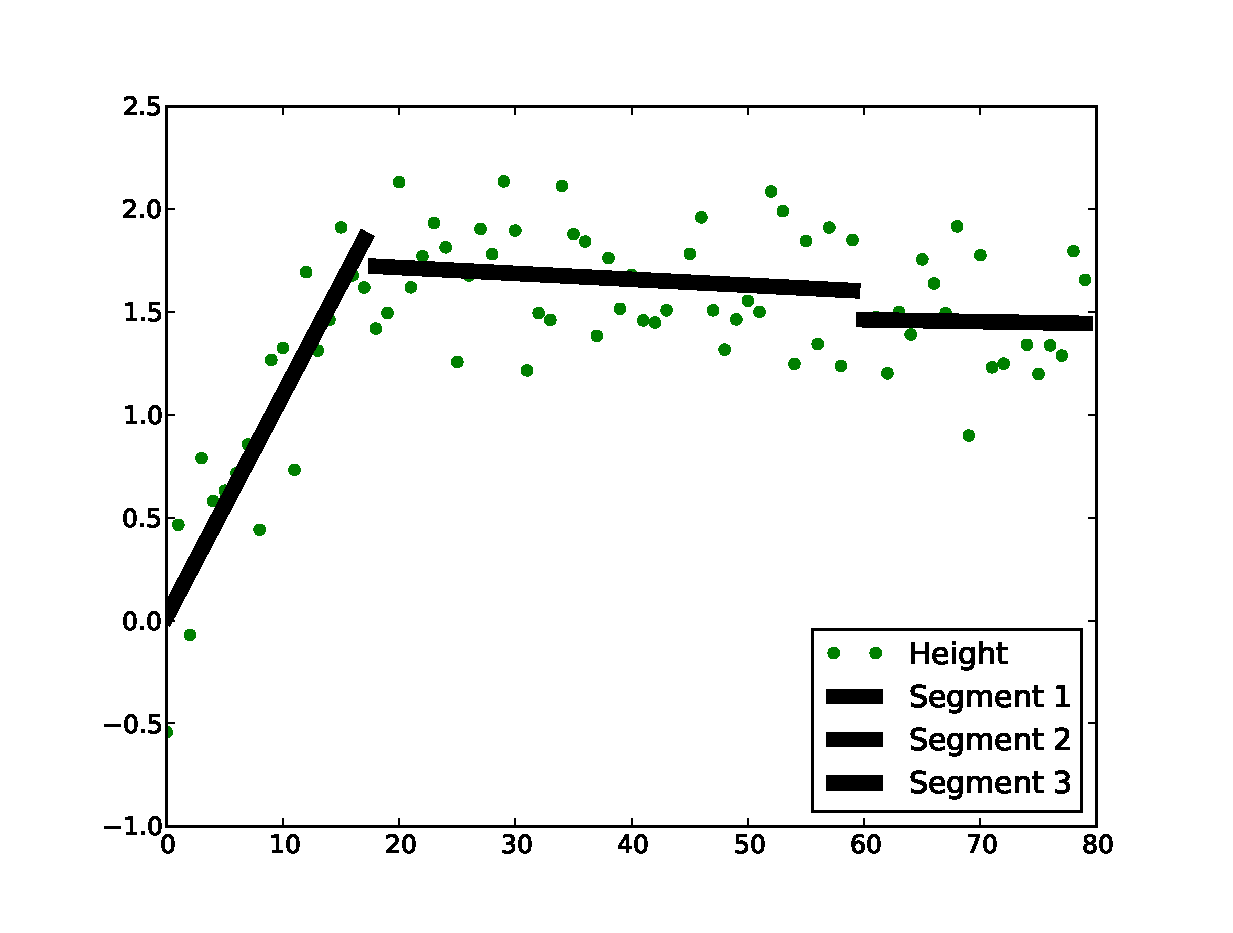
\includegraphics[width=0.5\textwidth]{../images/height_v_age_segmentfit}
  \caption{Left:  Fitting height vs. age with a linear function.  Right:  Fitting with a segmented function.  Fake data.}
\end{figure}
If we try to use height by itself, then it will have a hard time fitting this non-linear curve.  See figure \ref{linear:fig:mean-height} left.  A better alternative would be to put a nonlinear transformation of height.  Perhaps take the (sample) mean height as a function of age.  One more possibility is to \emph{segment} your model into three groups:  People between zero and eighteen, people between eighteen and sixty, and people older than sixty.  Then, three different models could be built.  Which is best?  If you are only using height, then using a mean curve would be better than segmenting, since, at best, the segments can only hope to achieve the mean.  When combined with other variables however, segmentation allows more room for the model to adjust since, e.g. the fit between eighteen and sixty won't effect the fit between zero and eighteen.  Segmenting has the disadvantage in that it requires splitting the data up into three smaller groups and keeping track of three models.

\section{Error Metrics}
To evaluate your model you need some metrics.  In our case, linear regression produces a point estimate $\hat w$.  From this it is easy to obtain a prediction $\hat Y = X\hat w$.  These can be compared in a few different ways.  Note that any method can be performed on the training set or a test/cross-validation set.

The most popular metric seems to be the \emph{coefficient of determination}, or $R^2$ (spoken as \emph{R-squared}).  This is defined as
\begin{align}
  1 - \frac{\|X\hat w - Y\|^2}{\|\bar Y- Y\|^2},
  \label{linear:align:R2}
\end{align}
where $\bar Y$ is the $N\times1$ vector with every entry equal to the mean of $Y$.  $R^2$ enjoys some nice properties, which we leave as an exercise.

\begin{exercise}
  Show that\ldots
\begin{enumerate}
  \item a perfect model ($X\hat w = Y$) will lead to $R^2=1$.
  \item if $X$, $Y$ are the training set, and $X$ contains a constant column, $0\leq R^2 \leq 1$.
  \item if $X$ does not contain a constant column, $R^2$ could in some cases be less than zero.
  \item if $X$ and $Y$ are not the training set, $R^2$ could in some cases be less than zero.
\end{enumerate}
\end{exercise}

$R^2$ has a few different interpretations.
\begin{enumerate}
  \item[(i)]  The denominator in the ratio in \eqref{linear:align:R2} can be thought of as the variability in the data.  The numerator can be thought of as the variability unexplained by the model.  Subtracting the ratio from one we get $R^2$, the \emph{fraction of variability explained by the model}.
  \item[(ii)] $R^2$ can also be thought of as \emph{the improvement from null model to the fitted model}.  We will generalize this idea later in the chapter on logistic regression.
  \item[(iii)] For linear models, $R^2$ is the \emph{square of the correlation} between the model's predicted values and the actual values.
\end{enumerate}

Since squaring a number smaller than one makes it smaller, and squaring a number larger than one makes it larger, $R^2$ will tend to penalize larger errors more.  More generally, define the \emph{L-p norm} as 
\begin{align*}
  \|X\hat w - Y\|_p :&= \left( \sum_{n=1}^N |X_{n:}\cdot \hat w - Y_{n:}|^p \right)^{1/p},
\end{align*}
and the \emph{L-infinity} norm as
\begin{align*}
  \|X\hat w - Y\|_\infty :&= \max\left\{ |X_{n:}\cdot \hat w - Y_{n:}| \right\}.
\end{align*}
If $p=1$ then we are computing ($N$ times) the \emph{mean absolute error}.

\begin{exercise}
  Show that\ldots
  \begin{enumerate}
    \item as $p\to\infty$, $\|X\hat w - Y\|_p\to \|X\hat w - Y\|_\infty$.  In other words, as $p$ increases we are penalizing the larger deviations more and more
    \item as $p\to0$, $\|X\hat w - Y\|_p$ tends to the number of elements of $X\hat w$ and $Y$ that differ.  In other words, decreasing $p$ penalizes all deviations equally.
  \end{enumerate}
\end{exercise}

\begin{exercise}
  Suppose we fit two linear regression models using two different datasets, $(X,Y)$ and $(X', Y')$.  Both data sets are the same length.  We notice that the $R-square$ error is bigger with $(X, Y)$ and the $L-2$ error is bigger with $(X', Y')$.  How can this be?
\end{exercise}


\section{End Notes}

An extensive introduction to similar material can be found in ``The elements of statistical learning'' by Hastie, Tibshirani, and Friedman\cite{HastieElements}.  The ``elements'' book covers more of the classical statistical tests (e.g. \emph{p-values}) which are important to understand since you will be asked to produce them.  Our theoretical treatment is designed to compliment this classical approach, and to prep you for the numerical problem.

For a more complete treatment of Bayesian prediction/inference, we refer the reader to the statistical text by Gelman \cite{GelmanBayesian}, and the machine-learning text by Bishop \cite{BishopPattern}.

A very theoretical treatment of regularization can be found in the book ``Regularization of Inverse Problems'' \cite{HeinzRegularization}.

\chapter{Logistic Regression}
\label{chapter:logistic}
\begin{center}
  {\Large\textit{The purpose of computing is insight, not numbers.\\- Richard Hamming}}
\end{center}
\vspace{0.2in}

\section{Formulation}

\emph{Logistic regression} is probably familiar to many of you, so we will try to formulate the problem from a few different angles.  

\subsection{Presenter's viewpoint}
Let's consider the viewpoint of a data scientist explaining logistic regression to a non-technical audience.  One challenge is that the dependent variable in the training data does not explicitly coincide with the model output.  For example, consider the data set \T{training.csv},

\begin{minted}{bash}
  age,dosage,recovers
  33,100,1
  22,90,0
  15,90,1
  23,85,0
\end{minted}

The variable in the column \T{recovers} is one when the subject recovers from cancer, and zero when they do not.  \T{dosage} is the dosage of some hypothetical drug.  A logistic regression could be used to take in age and dosage, and output the probability that the subject recovers.  In this case, our model output could look like

\begin{minted}{bash}
  age,dosage,prob_recovers
  33,100,0.85
  22,90,0.6
  15,90,0.7
  23,85,0.4
\end{minted}

So our model output is a probability $p\in[0,1]$, which does not match up with our dependent variable.  This is in contrast to the use of logistic regression for \emph{classification}.  Here for example, a cutoff is chosen such that if \T{prob\_recovers} $ > $ \T{cutoff}, then we classify the subject one that will recover.  If \T{cutoff} = 0.5, then out model output would be $(1, 1, 1, 0)$, which could be compared directly with the training data, as is the case with linear regression.

\subsection{Classical viewpoint}
The classic formulation of logistic regression starts with assumptions about the probability of $y$ taking either 0 or 1, given the value of $x$.  Let's write this as $\rmP[y=0\g x]$ and $\rmP[y=1\g x]$.  The assumption is
\begin{align}
  \log\left[ \frac{\rmP[y = 1\g x]}{1 - \rmP[y=1\g x]} \right] &=x \cdot w.
  \label{logistic:align:basic-assumption-1}
\end{align}
This can be re-written using the \emph{logit} function, defined by $\logit z := \log[z / (1-z)]$.  Solving for $\rmP[y=1\g x]$ we arrive at
\begin{align}
  \rmP[y=1\g x] &= \frac{e^{x\cdot w}}{1 + e^{x\cdot w}}.
  \label{logistic:align:basic-assumption-2}
\end{align}
This can also be re-written using the \emph{logistic sigmoid} function $\sigma(z) := \exp(z)/(1 + \exp(z))$.  In other words, our model assumes $\rmP[y=1\g x] = \sigma(x\cdot w)$.  This function has the nice property that it takes values in the interval $[0,1]$, as a probability should.  Moreover, it behaves nicely when differentiated (see exercise \ref{logistic:exercise:sigmoid}).
\begin{figure}
  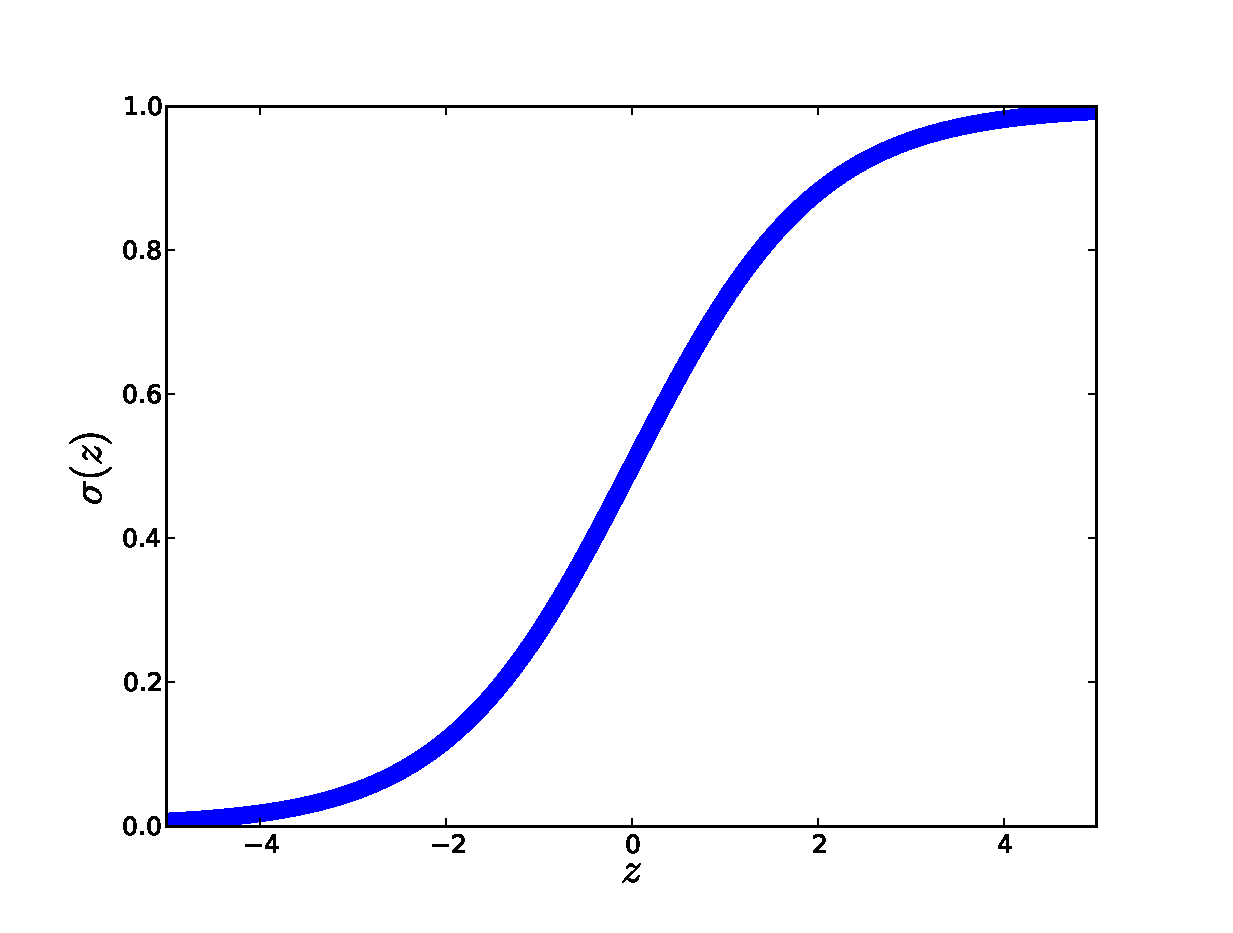
\includegraphics[width=0.7\textwidth]{../images/sigmoid}
  \caption{Plot of the sigmoid function $\sigma(z)$ from for $z\cdot w\in[-5, 5]$.}
\end{figure}

\begin{exercise}
  Show that \eqref{logistic:align:basic-assumption-1} implies \eqref{logistic:align:basic-assumption-2}.
\end{exercise}

\begin{exercise}
  \label{logistic:exercise:sigmoid}
  Show that $\sigma'(z) = \sigma(z)(1 - \sigma(z))$, and $\sigma(-z) = 1 - \sigma(z)$.
\end{exercise}

\subsection{Data generating viewpoint}
\label{logistic:subsection:data-generating-viewpoint}
One can devise a data generating process that gives rise to the classical viewpoint.  Suppose we have a latent variable $z$ such that our observed variable $y$ is given by $y := \one_{z>0}$.  For example, $y=1$ could indicate ``patient recovers from cancer'', and $z$ is the health level of the patient.  To tie this to independent variables we consider the model
\begin{align*}
  z &= x\cdot w + \eps,
\end{align*}
where $\eps$ is a random variable with probability density $\sigma'(z) = \sigma(z)(1 - \sigma(z))$ (see exercise \ref{logistic:exercise:sigmoid}).  This implies
\begin{align*}
  \rmP[y = 1] &= \rmP[z > 0] = \rmP[\eps > -x\cdot w] = \int_{-x\cdot w}^\infty \sigma'(\eta)\d\eta = \int_{-\infty}^{x\cdot w}\sigma'(\eta)\d\eta\\
  &= \sigma(x\cdot w),
\end{align*}
where the second to last equality is justified by verifying $\sigma'(z) = \sigma'(-z)$.  In other words, $y$ has probability mass function given by \eqref{logistic:align:basic-assumption-2}.

This formulation is useful because it allows one to explore questions of model error.  For example, suppose $\eps$ depends on $x$.  This could arise if there is error in some of the labels, and this error depends on $x$ (suppose it is more difficult to determine recovery in older patients).  More generally, $\eps$ represents the deviation of the latent variable $z$ from our modeled value $x\cdot w$.  Re-phrasing our conversation at the beginning of chapter \ref{chapter:linear}, there is no need to assume that the world is fundamentally random.  There exists some set of variables $(x, v)$ that tell us with certainty whether or not a person will recover (for example, the position and state of every particle in the universe).  It just happens that in our data set we do not have access to all of them (we only have $x$), or to the correct functional form of their relationship to the observed variable $\one_{z>0}$.  If there true form is $z = f(x, v)$, we can write
\begin{align}
  \label{logistic:align:model-error}
  z &= x\cdot w + \eps,\quad \mbox{ where }\quad\eps := x\cdot w - f(x,v).
\end{align}
In other words, $\eps$ represents the uncertainty in our model.


\begin{exercise}
  Referring to the paragraph above \eqref{logistic:align:model-error}, restate the issue of mislabeled data as a problem of modeling error.
\end{exercise}


\section{Determining the regression coefficient $w$}
Before we proceed, we should define a couple things.  A matrix $A$ is said to be \emph{positive definite} if it is symmetric and all of its eigenvalues are positive.  Rather than computing the eigenvalues, one can check that, for every nonzero vector $v$, $v^TAv>0$.  A function $f(w)$ is strictly convex if, for all $\lambda\in[0,1]$, and points $w^1, w^2\in\RK$, $f(\lambda w_1 + (1-\lambda)w_2) < \lambda f(w_1) + (1-\lambda)f(w_2)$.  If $f$ has two continuous derivatives, then, rather than checking the above inequality, one can check that the hessian matrix $\nabla^2f(w)$ is positive definite at every point $w\in\RK$.  If a function $f:\RK\to\Rone$ is strictly convex, then any local minimum is also the global minimum.  Note that it is possible for the function to not have any minimum (e.g. it can keep getting smaller and smaller as $w\to\infty$).  This is very important for optimization, since most algorithms are able to find local minimums, but have a hard time verifying that this is a global minimum.

The coefficient $w$ in \eqref{logistic:align:basic-assumption-1}, \eqref{logistic:align:basic-assumption-2} is usually determined by maximum likelihood, although a Bayesian approach may be used.  In either case, we need the likelihood.  Recalling the notation of chapter \ref{chapter:notation}, the likelihood is
\begin{align*}
  p(Y\g w) &= \prod_{n=1}^N p(Y_n\g w) = \prod_{n=1}^N \rmP[y=1\g x=X_{n:}, w]^{Y_n}\rmP[y=0\g x=X_{n:},w]^{1-Y_n}\\
  &= \prod_{n=1}^N \sigma(X_{n:}\cdot w)^{Y_n}(1-\sigma(X_{n:}\cdot w))^{1-Y_n}.
\end{align*}
This can be checked by considering the cases $Y_n=0$ and $Y_n=1$ separately.  The maximum likelihood solution is the point $w_{ML}$ that maximizes this.  Instead we usually minimize the negative log likelihood, that is
\begin{align}
  \label{logistic:align:ML-soln}
  \begin{split}
    w_{ML} :&= \arg\min_w L(w),\qquad\mbox{where,}\\
    L(w) :&= -\sum_{n=1}^N\left[ Y_n\log\sigma(X_{n:}\cdot w) + (1-Y_n)\log(1-\sigma(X_{n:}\cdot w)) \right].
  \end{split}
\end{align}
Note that $L(w)$ will always be non-negative since $\sigma\in(0, 1)$.
Since $\sigma'(z) = \sigma(z)(1-\sigma(z))$, we find that
\begin{align*}
  \frac{\p L}{\p w_k} &= \sum_{n=1}^N\left[ \sigma(X_{n:}\cdot w) - Y_n \right]X_{nk},\qquad
  \frac{\p^2 L}{\p w_k w_j} = \sum_{n=1}^N\sigma(X_{n:}\cdot w)(1 - \sigma(X_{n:}\cdot w)) X_{nk}X_{nj}.
\end{align*}
Or, with $\nabla L$ and $\nabla^2L$ denoting the gradient and hessian matrix (the matrix with $kj$ entry equal to $\p^2L/\p w_k\p w_j$),
\begin{align}
  \label{logistic:align:grad-hess}
  \begin{split}
    \nabla L(w) &= \sum_{n=1}^N\left[ \sigma(X_{n:}\cdot w) - Y_n \right]X_{n:},\\
    \nabla^2L(w) &= \sum_{n=1}^N\sigma(X_{n:}\cdot w)(1 - \sigma(X_{n:}\cdot w)) X_{n:}^TX_{n:}.
  \end{split}
\end{align}
One can check that for any vector $v\in\RK$,
\begin{align*}
  v\cdot\nabla^2L(w)v &= \sum_{n=1}^N(v\cdot X_{n:})^2\sigma(X_{n:}\cdot w)(1-\sigma(X_{n:}\cdot w)),
\end{align*}
which is greater than or equal to zero, and strictly greater than zero for all vectors provided the matrix $X$ has rank $K$.  In other words, if the data columns are linearly independent, then the hessian is positive definite for every $w$, and hence the function $L$ is strictly convex.  This implies that any local minimum of $L$ is a global min, which can be shown to be $w_{true}$ in the limit $N\to\infty$ if the rows $X_{n:}$ are statistically independent samples and the data generating process is as described in section \ref{logistic:subsection:data-generating-viewpoint} with $w=w_{true}$.  To make this last statement plausible, note that in this ideal case, the expected value of $\nabla L(w)$ is $\sum_n\left[ \sigma(X_{n:}\cdot w) - \sigma(X_{n:}\cdot w_{true}) \right]$, of which $w=w_{true}$ is the minimizing value.  Since $\nabla L(w)$ is a sum of random variables, we can rescale it by $1/N$ and see that it should approach its expectation.  

\begin{exercise}
  Show that for fixed $w$, $\nabla^2L(w)$ is positive definite for all $w$ if and only if $X$ has rank $K$.
\end{exercise}

\begin{digression*}[Don't truncate linear regression!]
  Suppose we are told to determine the probability that a customer will keep their membership with ``Super Fitness Gym'' for longer than one year.  We ask the general manager for data and she gives us height, weight, age, and \emph{length of gym membership in months} for 10,000 customers (ignore the fact that some customers have only been there less than a year and have not had the chance to be there a full year).  Now we have membership information as a semi-continuous variable \emph{membership-length}$ = 1,2,\dots$, but we are asked to predict a binary outcome (either Yes or No).  One approach would be to set $Y = 1$ if membership length is greater than 12, and 0 if it is less.  However, this approach throws out information about how long someone has been at the gym.  For example, people who quit in 1 month are treated the same as those who quit in 11.  A better approach would probably be to use a linear regression model where we try to predict the number of months that the membership will last.  To turn this into a probability, we would use a Bayesian approach to determine $p(y\g x, Y)$ as in section \ref{linear:subsection:generic} equation \eqref{linear:align:predictive}.  Since the data is discrete but ordered (1,2,3,\ldots) a better approach would be so called \emph{ordinal regression}.  Since some people have not quit (hence we don't know how long they will be there) the best approach would be \emph{right-censored ordinal regression}.
\end{digression*}

The Bayesian approach proceeds as in chapter \ref{chapter:linear}.  That is, we choose a prior $p(w)$ and form the posterior $p(w\g Y)\propto p(w)p(Y\g w)$.  Gaussian priors are common.  Also common is the Laplace prior $p(w)\propto \exp\left\{ -\alpha\|w\|_1 \right\}$, where $\|w\|_1 = \sum |w_k|$ is the L1 norm of $w$.  See section \ref{logistic:section:L1}.

\begin{exercise}
  Sometimes, otherwise well-meaning individuals, use linear regression to solve a logistic regression problem.  Consider the case of spam filtering.  Your independent variables are the num ber of times certain words appear in the document.  For example, the word ``V1@Gra'' is one of them, and of course this world is almost always associated with spam.  You are told to produce a model that gives the probability that an email is spam.  Your colleague, Randolph Duke, tells you that since the dependent variable $y$ is a number (in this case 0 or 1), he will build a linear regression that takes in $x$ and tries to predict $y$.  Of course the result won't be in the interval $[0, 1]$, but, \underline{after training}, he will truncate it, or re-scale it, so that it is.  What is wrong with Mr. Duke's approach?
\end{exercise}


\begin{exercise}[Heteroscedastic probit models]
  A \emph{probit regression} is just like a logistic regression, but rather than the logistic sigmoid $\sigma(x\cdot w)$, we use the Gaussian cumulative distribution function $\Phi(x\cdot w)$. 
  \begin{enumerate}
    \item Following the reasoning in section \ref{logistic:subsection:data-generating-viewpoint}, show that if $y = \one_{z>0}$ with $z = x\cdot w_{true}+\eps$ with $\eps\sim\calN(0, \lambda^2)$ being \iid, then  $\rmP[y=1\g x] = \Phi(x\cdot w_{true}/\lambda)$.
    \item If we perform a probit regression, we will assume $\rmP[y=1\g x] = \Phi(x\cdot w)$.  In other words, we will set $\lambda=1$.  From the standpoint of building a model that takes in $x$ and spits out $\rmP[y=1\g x]$, why doesn't the assumption $\lambda=1$ matter?
    \item Suppose now that $\eps \sim\calN(0, (x\cdot v_{true})^2)$.  Show that our model should be
      \begin{align*}
        \rmP[y=1\g x] &= \Phi\left( \frac{x\cdot w}{x\cdot v} \right).
      \end{align*}
    \item Using the notation
      \begin{align*}
        \Phi_n :&= \Phi\left( \frac{X_{n:}\cdot w}{X_{n:}\cdot v} \right),
      \end{align*}
      write down the likelihood and negative log likelihood associated to the independent variable matrix $X$ and dependent variable vector $Y$.
  \end{enumerate} 
  Minimizing the negative log likelihood is obviously more difficult because it involves a nonlinear combination of variables.  For that reason, an iterative technique is used, whereby $v$ is fixed and the minimum over $w$ is obtained, then $w$ is fixed and a minimum over $v$ is obtained.  This iterative procedure is repeated until the negative log likelihood stops changing very much.
\end{exercise}

\section{Multinomial logistic regression}
\label{logistic:section:multinomial}
Logistic regression can be generalized to the case where $y$ takes on a number of values.  Call each of these classes $C_m$ for $m=1,\cdots,M$.  We can generalize \eqref{logistic:align:basic-assumption-1} to get
\begin{align*}
  \log\frac{\rmP[y=C_i\g x]}{\rmP[y=C_M\g x]} &= x\cdot w^i,\qquad i = 1,\cdots,M-1.
\end{align*}
The coefficients $w^i$, for $i=1,\cdots,M-1$, are each vectors in $\RK$, viz. $w^i=(w^i_1,\cdots,w^i_K)$.  One can solve for the probabilities and arrive at a generalization of \eqref{logistic:align:basic-assumption-2},
\begin{align}
  \label{logistic:align:basic-multinomial-assumption}
  \rmP[y=C_i\g x] &= \frac{\exp\left\{ x\cdot w^i \right\}}{1 + \sum_{m=1}^{M-1}\exp\left\{x\cdot w^m\right\}}.
\end{align}

The coefficients are determined in a manner similar to two-class logistic regression.  That is, we write down a likelihood (or posterior) and maximize it using information about the gradient and possibly the hessian.

\begin{digression*}[Multinomial versus ordinal]
  Suppose we build a model for the number of goals scored in a soccer game.  Since this number is typically something like 1, 2, 3, or 4, it does not make sense to use linear regression.  One approach would be to build a multinomial logistic model where the classes are defined as follows.  $C_1$ represents ``team scored 1 or less goals'', $C_2$, and $C_3$ represent ``team scored 2, or 3 goals'', and $C_4$ represents ``team scored 4 or more goals.''  We could then train the model and recover coefficients for each class, $w^1,\cdots,w^4$.  This however is not a good approach.  The main problem lies in the fact that the class probabilities \eqref{logistic:align:basic-multinomial-assumption}, and hence the coefficients $w^i$, are not related in the proper way.  They are related in the sense that they sum to one (which is good), but this problem is special.  An increase in the qualities that allow a team to score 2 points will likely result in them scoring 3 (or more) points.  In other words, the quality of a team appears on some sort of continuum.  An ordinal model captures this extra structure and allows us to build a better model.
\end{digression*}

\section{Logistic regression for classification}

Logistic regression can be used for classification by choosing a cutoff $\delta\in[0,1]$ and classifying input $X_{n:}$ as class 1 (e.g. $y=1$) if $\sigma(X_{n:}\cdot w) > \delta$, and class 0 if $\sigma(X_{n:}\cdot w) \leq \delta$.  If $\delta=0.5$, then we are classifying $X_{n:}$ as class 1 precisely when our model tells us that ``the probability $Y_n=1$ is greater than 0.5.''  This is a good choice if we want to be correct most of the time.  However, other cutoffs can be used to balance considerations such as true/false positives.  See chapter \ref{chapter:text}.

Logistic regression as a classifier uses a hyperplane to separate $\RK$ into two regions, one of which we classify as ``class 0'', and the other ``class 1.''  See figure \ref{logistic:figure:separating-hyperplane}.
\begin{figure}
  \label{logistic:figure:separating-hyperplane}
  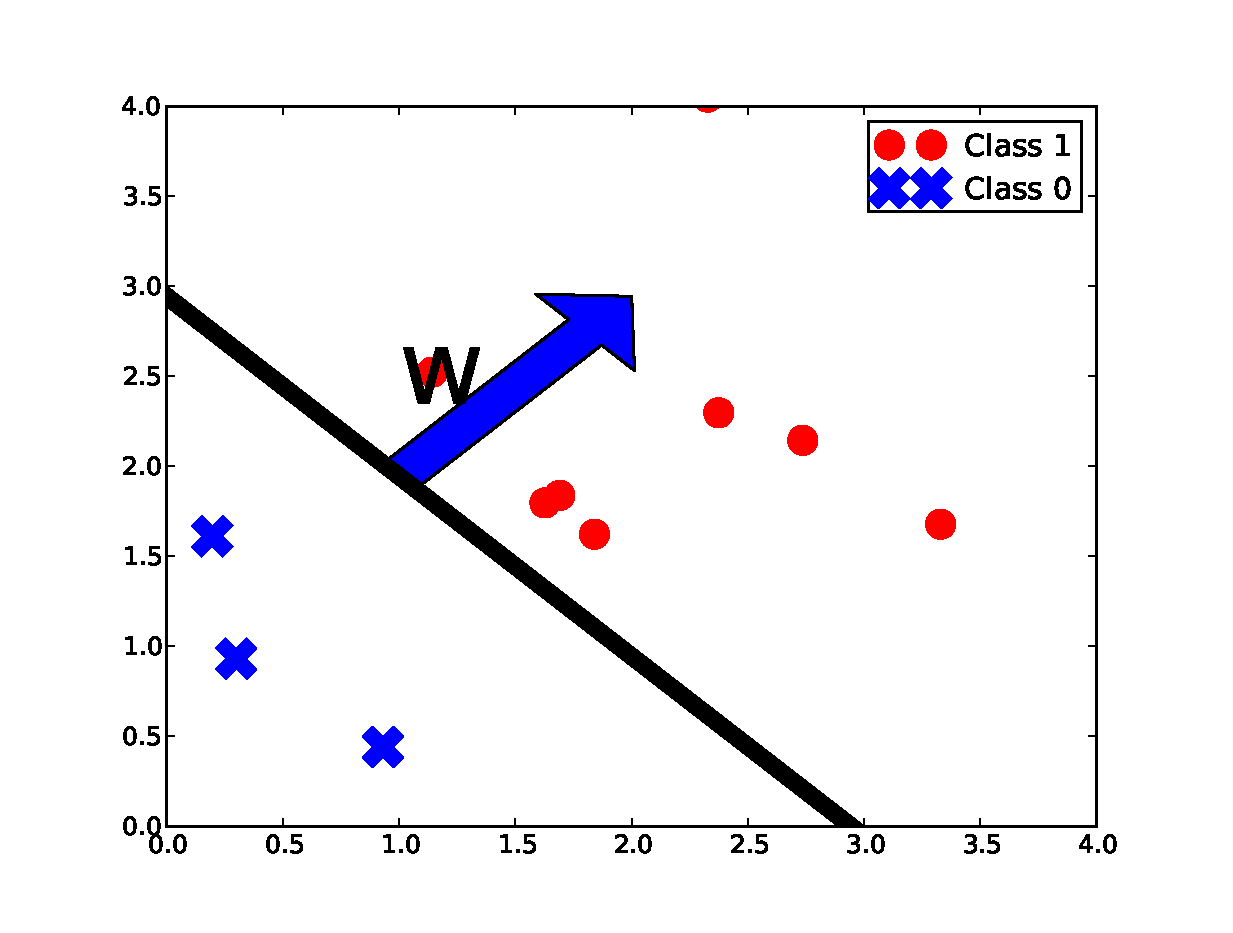
\includegraphics[width=0.7\textwidth]{../images/logistic_classifier}
  \caption{The hyperplane normal to $w$ separates space into two classes.  Whether or not this separation is correct is another story.}
\end{figure}
This happens because 
\begin{align*}
  \sigma(x\cdot w) > \delta &\quad\Leftrightarrow\quad x\cdot w > \log\frac{\delta}{1-\delta},
\end{align*}
and the set of points $x$ for which $x\cdot w$ is greater/less than some constant $c$ is the two regions on either side of the hyperplane defined by $x\cdot w = c$.  This fact is important because it is a fundamental limitation of logistic classification.  This sort of limitation is not present in other methods such as decision trees.  Note that the limitation may be a good thing if you know that the solution structure is roughly approximated by space separated by a hyperplane.  In a sense, this is a form of regularization, and prevents logistic regression from giving a ``crazy'' answer.  Also note that you are free to choose nonlinear combinations of variables, e.g. you can square some feature.  Then, in the original feature space, your separating hyperplane would be a curve.

\section{L1 regularization}
\label{logistic:section:L1}

As in section \ref{linear:section:bayesian}, we can choose a prior and form the posterior $p(w\g Y)\propto p(w)p(Y\g w)$.  As with linear regression, a Gaussian prior ($w\sim\exp{-\|w\|^2/(2\sigma_w^2)}$) is popular.  In this section we explore the consequences of choosing a Laplacian prior.  The \emph{Laplace} distribution has density function
\begin{align*}
  p(w) &\propto \exp\left( -\alpha\|w - \mu\|_1 \right), \qquad \|w\|_1 := \sum_{k=1}^K |w_k|.
\end{align*}
As with Gaussian priors, we will usually choose not to regularize the constant, and choose $\mu=0$.  In fact, we may wish to weight each term differently, in which case we will use the prior
\begin{align*}
  p(w) &= \exp\left( -\sum_{k=1}^K\alpha_k|w_k| \right), \qquad 0\leq\alpha_k<\infty.
\end{align*}
The MAP estimate is then
\begin{align}
  w_{MAP} :&= \arg\min_w\left\{ L(w) + \sum_{k=1}^K\alpha_k|w_k| \right\}.
  \label{logistic:align:map}
\end{align}
Solving for $w_{MAP}$ is known as using a Laplace prior, \emph{Lasso}, or \emph{L1 regularization}, and is related to the field of \emph{compressed sensing}.

\begin{exercise}
  Show that the MAP estimate is given by \eqref{logistic:align:map}.
\end{exercise}

As with the Gaussian MAP in linear regression, \eqref{linear:align:regularized-lsq}, the term $\sum_k\alpha_k|w_k|$ penalizes large $w$.  The effect is different in a number of ways though.  First of all, for large $|w_k|$, the $|w_k|\ll|w_k|^2$, so the penalty is smaller.  This means that the L1 regularized solution allows for larger $w_k$ than the L2 regularized solution.  Second, the optimization problem \eqref{logistic:align:map} is significantly more difficult than \eqref{linear:align:regularized-lsq} because the terms $|w_k|$ are not differentiable.  Third, and most importantly, roughly speaking, L1 regularization results in insignificant coefficients being set \emph{exactly} to zero.  This is nice because it effectively removes them from the model, which means that the effective model can be significantly simpler than in L2 regularization.  More precisely,
\begin{theorem}
  \label{logistic:theorem:L1-selection}
  With $L(w)$ the negative log likelihood given by \eqref{logistic:align:ML-soln}, suppose that the columns of the data matrix $X$ are linearly independent and that $\alpha_k>0$ for all $k$.  Then the solution $w^\ast$ to \eqref{logistic:align:map} exists and is unique.  Moreover, for every $k$, exactly one of the following holds:
  \begin{enumerate}
    \item[(i)] 
      \begin{align*}
        \left|\frac{\p L}{\p w_k}(w^\ast)\right| &= \alpha_k \quad\mbox{ and }\quad w^\ast_k\neq0
      \end{align*}
    \item[(ii)]
      \begin{align*}
        \left|\frac{\p L}{\p w_k}(w^\ast)\right| &\leq \alpha_k \quad\mbox{ and }\quad w^\ast_k=0.
      \end{align*}
  \end{enumerate}
\end{theorem}
\begin{remark}
  %Suppose we are in case (ii), then theorem \ref{logistic:theorem:L1-selection} allows for $|\p_kL(w^\ast)|$ exactly equal to $\alpha$.  However, this is a pathological case since nothing is pulling 
  This means that $\alpha_k$ sets a level at which the coefficient $k^{th}$ variable must effect the log likelihood in order for its coefficient to be nonzero.  This is contrasted with L2 regularization, which tends to result in lots of small coefficients.  This can be expected since, for small $|w_k|$, the penalty $|w_k|\gg|w_k|^2$.  In fact, one could use terms such as $|w_k|^\beta$, for $0<\beta<1$ and achieve even more sparsity.  In practice this would lead to difficulty since the problem would no longer be convex.
\end{remark}
\begin{proof}
  Since the likelihood is bounded (it is always less than one), $L(w)$ is always greater than zero.  Let $M = \max\left\{ L(w)\st |w|<1 \right\}$ and $\alpha_m:=\min\left\{ \alpha_1,\cdots,\alpha_K \right\}$.  Then, for $|w|>M/\alpha_m$ we will have 
  \begin{align*}
    L(w) + \sum_k\alpha_k|w_k| & > \sum_k\alpha_k|w_k| > \alpha_m\sum_k|w_k| > \alpha_m|w| > M.
  \end{align*}
  In other words, a local minimum must occur in the set $\left\{ w\st |w| \leq M/\alpha_m \right\}$.  Since $L$ is strictly convex, and the penalty is convex, $L(w) + \sum_k\alpha_k|w_k|$ is strictly convex and this is a global minimum and the unique solution to the optimization problem.

  The rest of the proof proceeds by linearizing $L(w)$ around the optimal point $w^\ast$.  The reader is encouraged to consider a one-dimensional problem ($w\in\Rone$) and replace $L(w)$ with $L(w^\ast) + (w-w^\ast)L'(w^\ast)$ and consider the consequences.

  Continuing with the proof, define $f(w) := L(w) + \sum_k\alpha_k|w_k|$.  Suppose that $w^\ast_k\neq0$.  Then the derivative $\p_kf(w^\ast)$ exists, and since $w^\ast$ is a minimum it must be equal to zero.  This implies (i).  To show that (ii) is a possibility, consider the function $L(w) = cw + w^2$ with $0<c\leq\alpha$ for one-dimensional $w$.  One can verify that $w^\ast=0$, and $|L'(0)| = c$, so both inequality and equality are possible.  
  
It remains to show that no situation other than (i) or (ii) is possible.  This will follow from the fact that we can never have $|\p_kL(w^\ast)| > \alpha$.  To this end, assume that $0\leq\alpha_k<c<\p_kL(w)$ (the case of negative derivative is similar).  We then have, (with $e_k$ the standard Euclidean basis vector),
\begin{align*}
  f(w + \delta e_k) &= f(w) + \delta\frac{\p L}{\p w_k}(w) \pm\delta\alpha + o(\delta)\\
  &< f(w) - \delta|c-\alpha| + o(\delta)\\
  & < f(w) \qquad\mbox{ for $\delta$ small enough}.
\end{align*}
For small enough $\delta$, we must have $f(w + \delta e_k) < f(w)$, which means $w$ is not a minimum.  This completes the proof.
\end{proof}

It should be mentioned that the problem of finding the MAP estimate \eqref{logistic:align:map} is equivalent to solving the constrained problem
\begin{align*}
  \wstar :&= \arg\min_w L(w),\qquad\mbox{subject to}\\
  \sum_{k=1}^K\alpha_k|w_k| &\leq C,
\end{align*}
for some $C$ that depends on both $\alpha$ and the function $L$.  This dependence cannot be known before solving at least one of the problems.  However, the set of values taken by the coefficients as $C$ and $\alpha$ are swept from 0 to $\infty$ (a.k.a. the \emph{path}) is the same.  Since normal cross-validation practice involves sweeping the coefficients and evaluating the models, the two methods can often be used interchangeably.

\section{Numerical solution}
\label{logistic:section:numerical}
Unlike the linear regression problem of chapter \ref{chapter:linear}, which reduced to solving a linear system, logistic regression is a nonlinear optimization problem because the \emph{objective} function (the function to be minimized) $L(w) + \sum_k\alpha_k|w_k|$ can not be reduced to solving a linear system.  In this chapter we explore iterative methods for finding a solution.  These methods give us a sequence of values $w^0,w^1,\cdots$ converging to a local minimum $\wstar$ of the objective function $f(w)$.  Each $w^j$ is found by solving a local approximation to $f$.  Note that convexity is needed to assure us that this is a global minimum.

\subsection{Gradient descent}
Perhaps the simplest method for finding a minimum of a differentiable objective function $L(w)$ is \emph{gradient descent}.  This method can be motivated by observing that, locally, a function decreases most in the direction opposite to its gradient (which is the direction of greatest local increase).  So, in our iterative search for $\wstar$, we should move in the direction opposite the gradient at our current point, see algorithm \ref{logistic:algorithm:gradient-descent} and figure \ref{logistic:figure:grad-desc}.
\begin{algorithm}
  \label{logistic:algorithm:gradient-descent}
  \caption{Gradient descent}
\begin{algorithmic}
  \State Initialize $w^0$ to some point, set $j=0$
  \State Choose $\gamma_0>0$
  \State Choose a tolerance $tol$
  \While{$err > tol$}
    \State Compute $\nabla L(w^j)$
    \State Set $w^{j+1} \gets w^j - \gamma_j\nabla L(w^j)$
    \State Set $err = |w^{j+1} - w^j|$
    \State Choose $\gamma_{j+1}$ according to some criteria
    \State Set $j\gets j+1$
  \EndWhile
\EndWhile
\end{algorithmic}
\end{algorithm}
The parameter $\gamma_j$ in algorithm \ref{logistic:algorithm:gradient-descent} can be chosen in a number of ways.  
To prevent overshooting, it is sometimes shrunk according to some criteria.  Other times, we can choose it by minimizing the one dimensional function $g(\gamma) = L(w^j - \gamma \nabla L(w^j))$.  This search is a one-dimensional optimization, and can be done using e.g. Newton's method.
\begin{figure}
  \label{logistic:figure:grad-desc}
  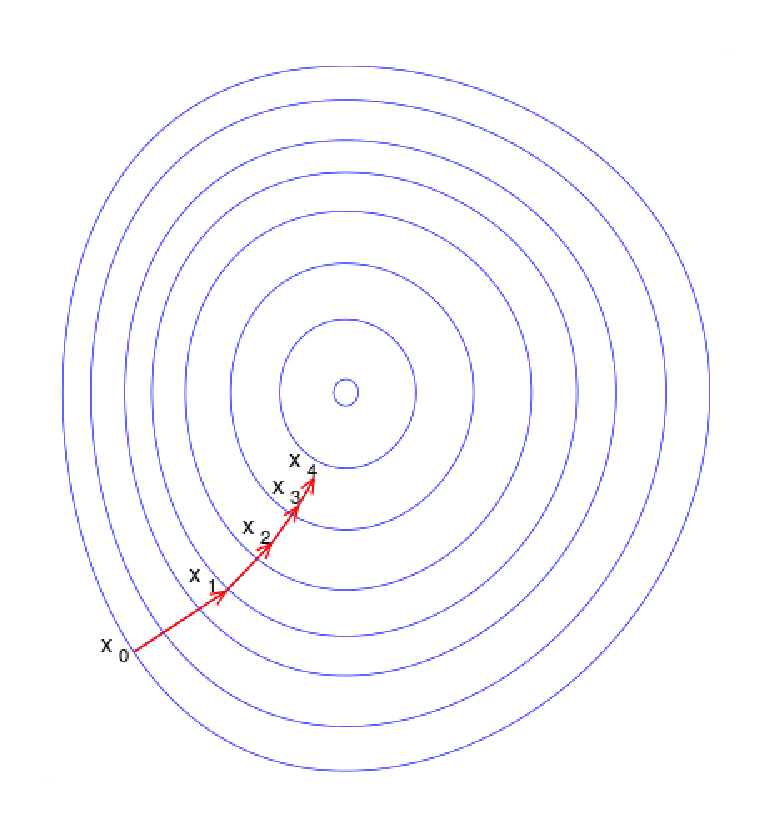
\includegraphics[width=0.5\textwidth]{../images/Gradient_descent}
  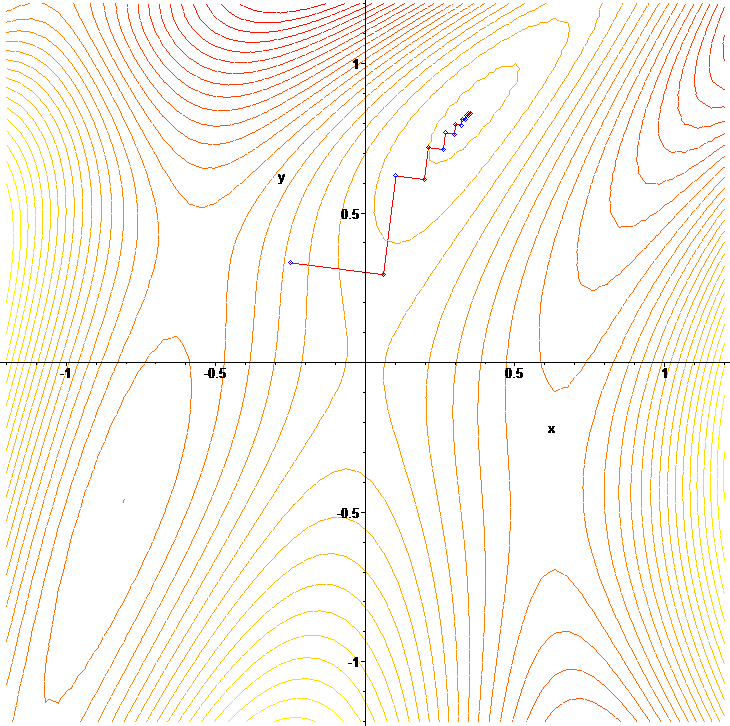
\includegraphics[width=0.5\textwidth]{../images/Gradient_descent_pathological}
  \caption{Contours show the level curves of functions.  Left:  Typical gradient descent path.  Right:  Pathological example where gradient descent zig-zags all over the place.}
\end{figure}
Gradient descent has the advantage of being very simple, and only requiring computation of the gradient.  It has the disadvantage of the fact that although the negative gradient is \emph{locally} the direction of biggest decrease in $L$, it often is not the best global direction.  In some cases, a gradient descent method can zig-zag around, missing the optimal solution, and take very long to converge.  See figure \ref{logistic:figure:grad-desc}.  Gradient descent should never be used for linear problems, since far superior methods exist here.  Another disadvantage is that it does require the gradient, which is not possible for some problems, e.g. L1 regularized regression.

\subsection{Newton's method}
For smooth objective functions where the hessian is not too difficult to compute, Newton's method is a very attractive option.  Newton's method finds zeros of functions (points where the function equals zero).   We can use Newton's method to find a minimum of $L$, since if $L$ is smooth, then at a local minimum we will have $\nabla L(\wstar)=0$.  So to optimize, we search for a zero of the gradient (and hence have to compute the hessian).  

To motivate Newton's method consider the problem of finding a zero of a one-dimensional function $g(w)$.  Suppose we are at point $w^j$ and want to find a new point $w^{j+1}$.  Approximate $g$ with the first term in its Taylor series,
\begin{align*}
  g(w) &\approx g(w^j) + (w - w^j)g'(w^j).
\end{align*}
Set this equal to zero, and get
\begin{align*}
  w^{j+1} &= w^j - \frac{g(w^j)}{g'(w^j)}.
\end{align*}
This leads to algorithm \ref{logistic:algorithm:newton-1d}
\begin{algorithm}
  \begin{algorithmic}[1]
    \caption{Newton's method for root finding (1-D)}
    \label{logistic:algorithm:newton-1d}
    \State Choose a starting point $w^0$, set $j\gets0$
    \State Choose a tolerance $tol$
    \While{$err > tol$}
        \State Compute $g'(w^j)$
        \State Set 
        \begin{align*}
          w^{j+1} &\gets w^j - \frac{g(w^j)}{g'(w^j)}.
        \end{align*}
        \State Set $err = |w^{j+1} - w^j|$
        \State Set $j\gets j+1$
    \EndWhile
  \end{algorithmic}
\end{algorithm}
In other words, at each point $w^j$, we form a linear approximation to $g(w)$, and use this to find the point at which this linear approximation is zero.

In the context of optimization, we are looking for a point where $L'(\wstar)=0$, so replace $g(w)$ with $L'(w)$ and you get the iteration step $w^{j+1} = w^j - L'(w^j)/L''(w^j)$.  In multiple dimensions, this is algorithm \ref{logistic:algorithm:newton-optimization}.
\begin{algorithm}
  \begin{algorithmic}[1]
    \caption{Newton's method for optimization}
    \label{logistic:algorithm:newton-optimization}
    \State Choose a starting point $w^0$, set $j\gets0$
    \State Choose a tolerance $tol$
    \While{$err > tol$}
        \State Compute $\nabla L(w^j)$, $\nabla^2L(w^j)$
        \State Set 
        \begin{align*}
          w^{j+1} &\gets w^j - (\nabla^2L(w^j))^{-1}\nabla L(w^j).
        \end{align*}
        \State Set $err = |w^{j+1} - w^j|$
        \State Set $j\gets j+1$
    \EndWhile
  \end{algorithmic}
\end{algorithm}

If all is well and $\nabla^2L(\wstar)$ is positive definite, then convergence to $\wstar$ is quadratic.  In this case that means $|w^{j+1}-\wstar| \leq C |w^j - \wstar|^2$ for some constant $C>0$.  If $\nabla^2L(\wstar)$ is not positive definite, then convergence can be very slow.  This, along with the need to compute and invert the hessian, are the major drawbacks of Newton's method for optimization.

\subsection{Solving the $L1$ regularized problem}
While gradient descent and Newton's method are available for maximum likelihood estimation, the L1 regularized problem requires special care (since it isn't smooth).  One technique (of many) is to transform the our MAP problem (which is unconstrained, and nonsmooth in $K$ unknowns)
\begin{align}
  \label{logistic:align:L1-again}
  \wstar :&= \arg\min_w \left\{ L(w) + \sum_{k=1}^K\alpha_k|w_k| \right\}
\end{align}
to the equivalent constrained, smooth problem in $2K$ unknowns
\begin{align}
  \label{logistic:align:L1-reformulated}
  \begin{split}
    (\wstar, \ustar) :&= \arg\min\left\{ L(w) + \sum_{k=1}^K\alpha_ku_k \right\},\\
    \mbox{subject to: }& -u_k\leq w_k \leq u_k,\qquad k=1,\cdots,K.
  \end{split}
\end{align}
Of course we don't care about the ``dummy'' variables $\ustar$, and they can be thrown away once the problem is done (they should equal $|w_k|$ at the minimum).

\begin{exercise}
  Show that if $(\wstar, \ustar)$ is a solution to \eqref{logistic:align:L1-reformulated}, then $\wstar$ is also a solution to \eqref{logistic:align:L1-again}.  
\end{exercise}

To solve \eqref{logistic:align:L1-reformulated}, a variety of approaches can be taken.  Since the objective function has at least two continuous derivatives, it is possible to replace it with a quadratic approximation (keep the first two terms in a Taylor series), get a best guess, then iterate.  This is the same goals as Newton's method, except here we have to deal with constraints.  A discussion of how this is done is beyond the scope of this text.

\subsection{Common numerical issues}
Here we discuss common numerical issues encountered when solving the maximum likelihood problem \eqref{logistic:align:ML-soln}.

\emph{Perfect separation} occurs when some hyperplane perfectly separates $\RK$ into one region where all training points have label 0, and another region where training points have label 1.  As an example, consider a one-dimensional logistic regression where we have two training data points:

\begin{tabular}{|l|r|}
  \hline
  X & Y \\
  \hline
  -1 & 0 \\
  \hline
  1 & 1 \\
  \hline
\end{tabular}

Before we write any equations, what do you think will happen?  Remember that this is not a Bayesian model, and it tries to fit the training data as well as it can.  From the model's perspective, it thinks that if $x=-1$, then $y$ will \underline{always} be zero!  Moreover, if $x=1$, the model thinks $y$ will always be 1.  What will our model say about the other points?  As it turns out, the maximum likelihood solution is $w=\infty$ (if you can call this a solution, since no computer will ever reach this point), and the model will say that any negative point $x$ will correspond to $y=0$ with 100\% certainty, and that any positive point $x$ will correspond to $y=1$ with 100\% certainty.
\begin{exercise}
  Consider a logistic regression problem with training data as above.  Note that we will not use a constant in this model.  
  \begin{enumerate}
    \item Show that for any $w\in\Rone$, $L(w+1)< L(w)$, and that as $w\to\infty$, $L(w)$ decreases to $0$.  This means that the maximum likelihood ``solution'' is $w_{ML}=\infty$.
    \item Show that this could not happen if you used $L1$ or $L2$ regularization.
    \item Draw the function $\sigma(x\cdot w)$ for $w = 10000000$, and $x\in[-3, 3]$.
    \item What is a separating hyperplane for this problem?
  \end{enumerate}
\end{exercise}

When perfect separation occurs, the numerical solution cannot converge.  A good solver will detect that $|w|\to\infty$ and will give you a warning.  The question for the modeler is, ``what to do next?''  It is possible that you included too many variables, since, if you have as many variables as you have data points (and all data points are unique), then you will always be able to find a separating hyperplane.  In this case, it makes sense to remove variables or increase the number of data points.

The next issue is specific to Newton's method.  Recall the expression for the hessian \eqref{logistic:align:grad-hess} and the discussion following it.  This showed that if there is linear dependency in the columns of $X$, then the hessian will be singular.  This will cause an error in Newton's method.  What to do?  You could regularize, which would eliminate this error.  You could also switch to a solver that did not require inversion of the hessian.  Our viewpoint however is that a singular hessian points to redundancy in the data, and that finding and eliminating that redundancy should be the first priority.  This can be done by eliminating columns from $X$ and checking if the rank of $X$ does not change.  If it does not change, then that column was redundant.
%Recall that, roughly speaking, Newton's method approximates $L(w) \approx L(\wstar) + \nabla L(\wstar) + \nabla^2L(\wstar)$, and solves for the minimum of this quadratic approximation.  

%The first Newton method specific issue is that, if there is linear dependency in the columns of $X$, then $\nabla^2L(w)$ will be singular for all $w$.  To make this plausible, consider the case where the first and second columns are exactly the same.  Since $L$ depends on $w_1$ and $w_2$ only through the algebraic term $w_1X_{n1} + w_2X_{n2} = (w_1 + w_2)X_{n1}$, changes in $w$ that preserve the term $w_1 + w_2$ make no difference.  Since these changes make no difference in $L$, they cannot possibly make a difference in $\nabla^2L$, which implies that $\nabla^2L$ will be singular.

%The second Newton method specific issue is slightly more subtle.  Suppose the first independent variable has absolutely no effect on $y$.  In this case, we do not expect $L$ to change when we change $w_1$, and therefore the first row and column of $\nabla^2L$ will be all zeros, which in turn implies that $\nabla^2L$ will be singular.  Of course, just by luck, changing $w_1$ will change $L$ a little bit, but this change will be very small when $N$ is large, and therefore $\nabla^2L$ will almost be singular.  A similar problem happens if two columns are almost the same, except for some noise that is unrelated to $y$.

\section{Model evaluation}

Linear regression can be thought of as a classifier that produces a probability of class inclusion.  This is no different than a Naive Bayes estimator, and the methods of section \ref{classification:subsection:roc} are applicable.  In particular, ROC curves are commonly used.  

The negative log likelihood is another candidate for measuring the goodness of fit.  The first difficulty arising with using the negative log likelihood is that it will increase in magnitude at a rate proportional to $N$.  This means we cannot hope to compare $L(w)$ for different size data sets. We can deal with this by dividing by $N$, giving the \emph{normalized negative log likelihood} $N^{-1}L$.  This is a good candidate to compare different models for the \emph{same} problem.  In other words, we can add/subtract variables and see how it effects $N^{-1}L$.  We can also compare $N^{-1}L$ in the training and test/cross-validation sets.

The normalized negative log likelihood $N^{-1}L$ does however depend quite a bit on the ``difficulty'' of the problem, and generally is not interpretable from problem to problem.  For this reason, it is usually not a meaningful quantity to share with people.  An alternative is the so-called (McFadden's) pseudo R-sqared,
\begin{align*}
  \Psi R2 :&= 1 - \frac{L(\wstar)}{L_{null}(\wstar)},
\end{align*}
where $L_{null}$ is the negative log likelihood obtained by using a model with \emph{only} a constant (the \emph{null model}).  Inspection of the definition reveals that $\Psi R2$ measures how much our full model improves on the null model.  Also, like $R$ squared, $0\leq\Psi R2\leq 1$.  Moreover, just like in linear regression, the ratio $L/L_{null}$ is the ratio of the negative log likelihoods.  This means that McFadden's pseudo R-squared is a generalization of $R^2$ from linear regression.  See bullet point (ii) below \eqref{linear:align:R2}.

\begin{exercise}
  Suppose your boss says, ``just figure out the R-square of your logistic regression model in the exact same way as you do for linear regression.''  Tell your boss why this is impossible.
\end{exercise}

\begin{exercise}
  Assume our ``full model'' (the one giving rise to $L$) is built with a constant and other variables.  Show that the in-sample $\Psi R2$ is between zero and one, with both zero and one as possible values.
\end{exercise}

\section{End Notes}

A great introduction to convex optimization has been written by Boyd and Vandenberghe.  It focuses on problem formulation and is hence applicable for users of the algorithms. \cite{BoydConvexOpt}.

\chapter{Models Behaving Well}
\label{chapter:models}
\begin{center}
  {\Large\textit{All models are wrong, some are useful.\\ \vspace{0.1in} - George Box}}
\end{center}
\vspace{0.2in}

Stories of modeling gone well and gone wrong.

Define:
\begin{itemize}
  \item Training model, production model
\end{itemize}

Tell stories about:
\begin{itemize}
  \item Newton's model for planetary motion
  \item Interpretability is more important than precision (story of black Scholes)
  \item Simplicity is more important than precision (Netflix story)
  \item Those who don't understand the math are doomed to use black boxes
  \item Your training model should be as close as possible to your production model (MBS modeling)
\end{itemize}

General remarks on:
\begin{itemize}
  \item Segregating data into training/cv/test sets
  \item Variable selection
  \item Transforming variables and why a linear-only model isn't enough
\end{itemize}



\section{End Notes}

The chapter title is a play on \emph{Models.Behaving.Badly}, by Emanuel Derman.  This book goes into much detail about the distinction between models and theory.


\part{Text Data}
\chapter[Processing Text]{Processing Text} 
\label{chapter:nlptext}
\begin{center}
%{\Large\textit{You just do it like that and shit works\ldots -I. Langmore}}
\end{center}
\vspace{0.2in}

%\section{History} 
%\label{text:history} 
%Something about where this comes from\ldots 

\section{A Quick Introduction}
%\begin{itemize}
%  \item Regular expressions
%  \item Text processing
%  \item Python NLTK library
%  \item Tokenization
%  \item Corpus
%  \item Python Pattern library
%\end{itemize}


With the influx of information during the last decade came a vast, ever growing, volume of \T{unstructured data}. An accepted definition of \T{unstructured data} is information that does not have a pre-defined data model or does not fit well into relational tables (if you have not seen relational database or tables, think of collection of python pandas data frames or similar containers). A large part of this category is taken up by text, which is what we will focus on in this chapter. 


From news publication, websites, emails, old document scans, social media the data world today is filled with text and many times it is up to the data scientist to extract useful information or usable signals. Much of this work falls into the realm of data processing and uses a variety of techniques from UNIX \t{regular expressions} to \T{natural language processing}. The following three are common examples: 

\begin{itemize}
    \item Text Classification: lets say you start with a collection of newspaper articles and the task is to properly place each into the appropriate news category. The task would be to first extract useful features from the text - these could be simply words, or nouns, or phrases - and then use these features to build a model.
    \item Web scraping: your task it to write a program that will crawl a number of websites, process the text and extract common themes, topics, or sentiment levels.
    \item Social media trends: your task is to analyze the reaction of twitter users to particular news events and to identifying those which are currently ``trending'' or have the potential of going ``viral.'' 
\end{itemize}

\section{Regular Expressions}
\label{regex}

Regular expressions \cite{WPRegEx} are an incredibly power tool for patter matching in text. 
They originated from automata and formal language theory of the 1950's and later, being integrated in \textit{Unix ed}, \textit{grep} 
and \textit{awk} programs, became an indispensable part of the Unix environment. The power of regular expressions comes from their flexibility and syntactical 
compactness; they form a language in their own right, which takes a bit of getting used to. However, with 
a little practice you become attuned to the internal logic and intelligent design. 

Python incorporates the regular expressions toolbox in a standard library called \textit{re}. You can find most of the 
information you will need at \\ http://docs.python.org/2/library/re.html. The library allows for added 
functionality on top of returning search patterns, such as boolean match function, replacement, etc

\subsection{Basic Concepts}

The easiest way to understand regular expressions is to begin using them, so lets start with an example. We are going to 
take a simple string of characters and extract some information from them. Hopefully you will have a terminal open
and can following along. 

\begin{minted}{python}
import re
myString = "<I am going to show 2 or maybe 10 examples
of using regular expressions.>"
re.findall(r"[a-zA-Z0-9]", mystring)    
\end{minted}

returns a list of every alphanumeric character that appears in the string above, i.e. we get a list of 57 characters from 'I' to 
s. As you can probably guess the code inside the parentheses simply asks for any character that is either a letter (any case) 
or a number. If we would like to include the period in this list, we can simply add it to the list of characters we are 
interested in.

\begin{minted}{python}
re.findall(r"[a-zA-Z0-9.]", s)    
\end{minted}

If we are interested in words, numbers included, and not just the individual characters we can include a "+" at the end of the expression, which is special as it 
matches one or more characters in the preceding regular expression, i.e.

\begin{minted}{python}
re.findall(r"[a-zA-Z0-9]+", s)    
\end{minted}

returns the list l = [`I',
 `am',
 `going',
 `to',
 `show',
 `2',
 `or',
 `maybe',
 `10',
 `examples',
 `of',
 `using',
 `regular',
 `expressions']. 


 Of course, typing character ranges explicitly as we did above can become a bit tedious, so there are special shorthand symbols to make life easier. For example
 we could have returned the above list by evoking

 \begin{minted}{python}
re.findall(r"\w+", s)    
\end{minted}

so now we know that `[a-zA-Z0-9]' = ``\textbackslash w'' in \textit{RE}. If we want all the symbols include the angled parentheses at the beginning and end of the string, we could 
call


 \begin{minted}{python}
re.findall(r".", s).    
\end{minted}

If are looking for all instances where a period appear, we could return that by calling

\begin{minted}{python}
re.findall(r"\.", s).    
\end{minted}

Hence, we have learned a few things about regular expression syntax: we have ways of matching certain characters, or ranges of characters; there 
is shorthand notation for common searches; there are special or "wild-card" characters, and ways of escaping those special characters (names by
calling "\textbackslash"). 

Now it's time to look at things a bit more formally. 



\subsection{Unix Command line and regular expressions}

We have already quite a bit about Unix command-line functions and utilities. You can think of Unix in terms of grammatical language structure, where:

\begin{itemize}
    \item commands like \textit{ls}, \textit{ls}, \textit{man} are thought of as verbs
    \item the objects, files, data to operate on as nouns
    \item shell operators, such as | or >, as conjunctions
\end{itemize}

so what we are missing now are some adjectives, and we can think of \textit{regular expressions} as filling this gap. We've already seen some regular expressions so lets look at a table of the core syntax. 

\begin{center}
    \begin{tabular}{c|l}
        \hline
        . & Match any character \\ \hline
        \^{} & Match the start of a string \\ \hline
        \$ & Match the end of a string or just before the newline character \\ \hline
            \textbackslash d & Match any decimal digit \\ \hline
            \textbackslash D &  Match any single non-digit character \\ \hline
            \textbackslash w & Match any single alphanumeric character  \\ \hline   
            [A-Z] & Match any of uppercase A to Z. \\ \hline
           ? &	Match zero or one occurrence of the preceding regular expression \\ \hline
            * &	Match zero or more occurrence of the preceding regular expression \\ \hline
            + &	Match one or more occurrences of the preceding regular expression. \\ \hline
            \{n\} &	Match exactly n occurrences of the preceding regular expression.\\ \hline
            \{m,n\} &	Match from m to n repetitions of the preceding regular expression \\ \hline 
            
        
    \end{tabular}
\end{center}

Lets look at some examples. Suppose you have a file \textit{people.txt} which contains the names of all the people in the class. It looks like:

\begin{minted}{bash}

Kate Student
Jake Student
Ian Professor
Emily Student
Daniel Professor
Sam Student
Chang Professor
Paul Student
\end{minted}

If you want something trivial such as retrieving all lines with professor names you can type

\begin{minted}{bash}
    grep Professor people.txt
\end{minted}

or even 

\begin{minted}{bash}
    grep Pr people.txt
\end{minted}

both of which return

\begin{minted}{bash}
Ian Professor
Daniel Professor
Chang Professor
\end{minted}

However, suppose you would like to do something slightly less trivial such as finding all people in the class whose name starts with the letter `P.' If you try something like

\begin{minted}{bash}
    grep P people.txt
\end{minted}

this will return 


\begin{minted}{bash}
Ian Professor
Daniel Professor
Chang Professor
Paul Student
\end{minted}


i.e. every line with a capital `P' in it. You can use regular expression to help out; do so you on some systems you will need to invoke the `E' flag 

\begin{minted}{bash}
    grep -E "^P" people.txt
\end{minted}

which will return 

\begin{minted}{bash}
Paul Student
\end{minted}

as desired. 


For another, perhaps more natural, example suppose you are a systems administrator and you need to find all login related processes as well as all processes corresponding to a certain user.  You can type

\begin{minted}{bash}
ps -e | grep -E "login|daniel"
\end{minted}

which will return the appropriate PID, time and command executed.


Lets look at a more interesting example. Suppose you have a big file and you would like to extract all lines which constitute a valid date, where a valid date is of the \textit{yyyy-mm-dd} format, between 1900-01-01 and 2099-12-31, with a choice of separators. Hence, we would accept character substrings \textit{2000-01-15} and \textit{2000/01/15}, but not \textit{2000/01-15}. The regular expression that would do this for you is



\begin{minted}{bash}
(19|20)\d\d[-/](0[1-9]|1[012])[-/](0[1-9]|[12][0-9]|3[01])
\end{minted}

This is a bit convoluted so lets fo through it. The first thing to notice is that there are three main groups
defined by brackers $()$; these are:

\begin{minted}{bash}
 (19|20)
 (0[1-9]|1[012])
 (0[1-9]|[12][0-9]|3[01])
\end{minted}

The first part just makes sure that you are looking for a string that starts with 19 or 20. The second group makes sure that you that the month starts with either a 0 or 1 and contunes with the appropriate digit, and similiar for the dates. In addition, we have a '\^{}' to signify that we are looking at the start of a line, then \d signifies we are looking for a number between 0 and 9, the $[- /.]$ which allows either a dash or a backslash. 

Note, there are some issues with this particular regular expression since it will match dates like \textit{2003-02-31}, but also it will match dates like \textit{2004/04-12} which you wanted to exclude. We'll see ways to get around this. 


\subsection{Finite State Automata and PCRE}

There are a number of different implementation of regular expressions, resulting in varied flexibility and performance. The ``original'' framework is modelled on \textit{finite state machines} \cite{WPFSM} making for a very fast and efficient approach. The complexity of finite automata implementation, referred to as \textit{re2}, is O(n) where n is the size of the input, but it does have its limitation. The main reason is that a finite state machine does not ``remember'' how it arrived at a given state, which prevents from evaluating a latter piece of a regular expression based on an earlier one. 

For example, suppose we have the following simple regex:

\begin{minted}{bash}
    "[ab]c+d"
\end{minted}

The machine will first check to see if there is ``a'' or ``d'' in the string, then whether it followed by one or more ``c"'s and then a ``d." Now by the time it makes to say ``d" it doesn't remember why it made it there, how many ``c"'s it encountered, or that this was preceded by an "a." You can visualize the situation with the following diagram

%\begin{displaymath}
%    \xymatrix{
%        \bullet \ar@/^/[r]
%        \ar@/_/@{.>}[r] &
%        \bullet }
%\end{displaymath}

This is precisely the limitation which prevented us from distinguishing between valid dates, i.e. those with either all "-" or "/" as separators, above.  One solutions is to extend the regular expression syntax to include \textit{backreferences}. The \textit{PCRE}, or \textit{Perl Compatible Regular Expressions}, implementation, which is what python \textit{RE} module was originally based on. However, matching regular expressions with backreference is an NP-hard problem.

\begin{figure}
  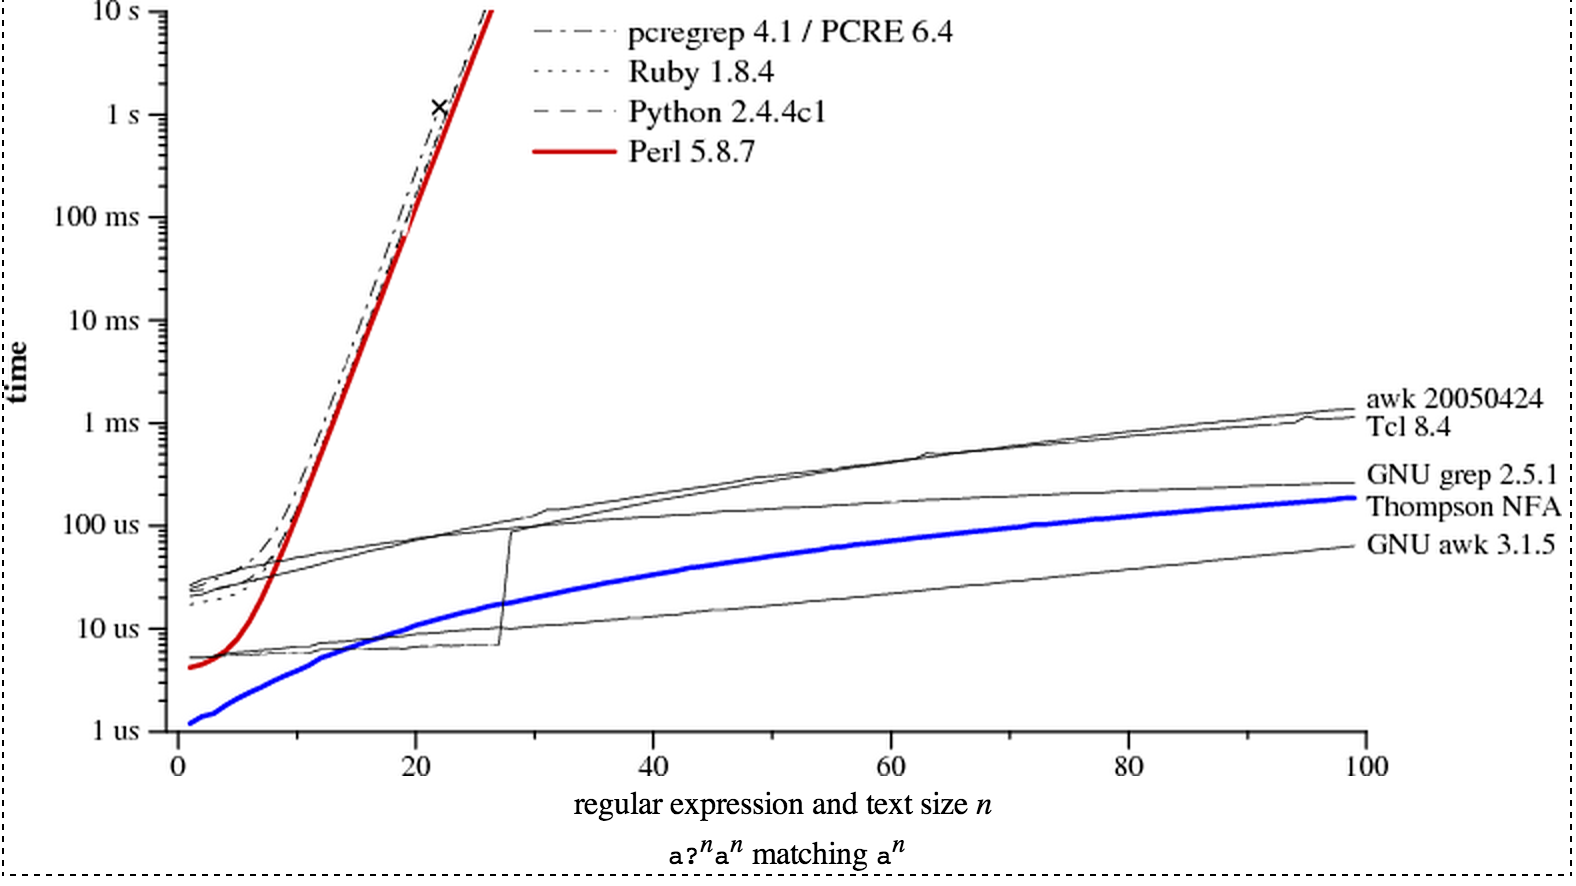
\includegraphics[width=\textwidth]{../images/RegExAlg}
  \caption{Regular Expression Implementation Time Comparison (see \cite{RegExComp} for more details)}
  \label{regex:regexALg}
\end{figure}






\subsection{Backreference} 

To mitigate the limitation of standard regular expression as described above, \textit{backreferences} were introduced. You can find these in the python \textit{RE} module as well as when calling grep with the -E flag (for \textit extended).

The basic syntax is quite simple, and is evoked by writing \textbackslash N to refer to the N'th group. If we refer back to the valid dates example from above we would replace the second set of [-/]'s with a backreference to first, ensuring a consistent match.

\begin{minted}{bash}
(19|20)\d\d([-/])(0[1-9]|1[012])\2(0[1-9]|[12][0-9]|3[01])
\end{minted}

Note that we are calling \textbackslash 2, because the first group is (19|20).

Of course, even backreferences don't solve all your problems, but they are big help. If you were trying to match something a bit more flexible such as balanced parentheses you would need a counter or just some additional scripting.


\begin{exercise}
    Use the python regular expression library to write a script that matches all lines in a file with balanced parentheses.
\end{exercise}


\section{Python RE Module}


The python regex library is an amazing tool that combines the power of regular expression, with backreference, and the flexibility of the python language. most of the syntax is inherited from unix, as above, but there are a few additions. 

There is also a large array of methods that come with the library, and a selection of the more noted is the following:

\begin{itemize}

    \item The findall function:

        
\begin{minted}{python}
re.findall(pattern, myString)
\end{minted}

        which returns all non-overlapping patterns in a string. For example,

\begin{minted}{python}
re.findall(r"\d+", "My number is 212-333-3333, and you can call 5-6pm")
\end{minted}

will return 

\begin{minted}{python}
["212", "333", "3333", "5", "6"]
\end{minted}




    \item The search function:

\begin{minted}{python}
re.search(pattern, myString)
\end{minted}

        which scans through a string and returns a \textit{re.MatchObject}, which always has a boolean value but also a number of methods. 
        For example, 

\begin{minted}{python}
myString = "My number is 212-333-3333, and you can call 5-6pm")
s = re.search(r"\d+", myString)
if s:
    print s.group(0)
\end{minted}

will print the number 212, since it is the first pattern match in the string. You can also do much more intelligent things with groups. For example, suppose you wan to check for the existence of a phone number and time and, if possible, return both. The following expression will do exactly that. 

\begin{minted}{python}
myString = "My number is 212-333-3333, and you can call 5-6pm")
s = re.search(r"(\d{3}-\d{3}-\d{4}).+(\d{1}-\d{1})(am|pm)", myString)
if s:
    print "this is the whole match:", s.group(0)
    print "this is the number:", s.group(1)
    print "this is the time:", s.group(2)
    print "this is the meridiem:", s.group(3) 
\end{minted}


Note, you can do a lot niftier things with groups in python's \textit{RE} module, such as attributing keys. For example,

\begin{minted}{python}
s = re.search(r"(?P\<number\>\d{3}-\d{3}-\d{4}).+(?P\<time\>\d{1}-\d{1})(?P\<ampm\>am|pm)", "My number is 212-333-3333, and you can call 5-6pm")
if s:
    print "this is the number:", s.group("number")
    print "this is the time:", s.group("time")
    print "this is the meridiem:", s.group("ampm")
\end{minted}




    \begin{digression*}[Difference between match and search]
        The only difference between re.match() and re.search() is the fact that match looks for patterns at the beginning of a string and search anywhere within. You can turn a search into a match function by appending a \^{} to the beginning of the patter at hand. 

    \end{digression*}


    \item The sub and split function. 

    
        These substitute a given found regex pattern with a string, or split on a given pattern. The basic syntax is

\begin{minted}{python}
    re.split(pattern, string)
    re.sub(patter, stringSub, string)
\end{minted}


\end{itemize}


\vspace{.5 in}

\newpage


\begin{digression*}[Why the "r?"]
    As you might have noticed there are two ways to enter a regular expression into a python \textit{RE} method, either in quotes or with a "r" appended to the front. The r invokes python's raw string notation and the reason for is that the use of backslash in regex to as an `escape' character, i.e. to allow special/wild characters to be used for a literal match, collides with python's use or a backslash for the same purpose in string literals. Hence, to match a backslash in a string using \textit{RE} you would have to write 

\begin{minted}{python}
re.findall("\\\\", myString),
\end{minted}

i.e. two backslashes to escape the special meaning in regex and two to escape it in python strings. If this were left so you can imagine a complete rigmarole, but luckily we can invoke the raw string notation and arrive at the same function with more sane syntax:

\begin{minted}{python}
re.findall(r"\\", myString)
\end{minted}


\end{digression*}



The python \textit{RE} library is very rich and incredibly powerful. We invite you to explore more on the module website \url{http://docs.python.org/2/library/re.html#re.MatchObject}.

\vspace{.5 in}


\begin{digression*}[fnmatch]

    In case you are wondering if there is a way to run unix shell-style wildcards from within python the answer is via the \textit{fnmatch} module. 
    For example, if you would like to print all filenames in a given directory with .txt extension, i.e. the equivalent of 

\begin{minted}{bash}
ls *.txt
\end{minted}

you can run

import fnmatch
import os

\begin{minted}{python}
for file in os.listdir('.'):
    if fnmatch.fnmatch(file, '*.txt'):
        print file
\end{minted}

Or if you would like to convert *.txt to it's regex equivalent

\begin{minted}{python}
regex = fnmatch.translate('*.txt')
\end{minted}

There are other modules that are great for handling paths and file extensions, such as glob, but the above can be useful from time to time. 


\end{digression*}


%\section{Text Processing}
%\label{textProc}


\section{The Python NLTK Library}
\label{nltk}

\subsection{The NLTK Corpus and Some Fun things to do}
\label{sub:nltk_corpus}

The NLTK library contains a large corpus, ranging from \textit{Moby Dick} to a collection of presidential inaugural addresses, which can be used for exploration of library, model development, etc/ 
You can see the work by typing 

\begin{minted}{python}
from nltk.book import *
texts()
\end{minted}


and explore individuals nltk.text objects by their designated text number. For example "text1" is nltk.text object containing 
\textit{Moby Dick}. Object method can be explored as usual by typing "text1. + tab" (if you are using ipython or and IDLE with tab 
completion). 

\begin{minted}{python}
from nltk.book import *
text.name
\end{minted}

\noindent returns "Moby Dick by Herman Melville 1851" and

\begin{minted}{python}
from nltk.book import *
text1.similar(`whale')
\end{minted}

\noindent returns 

\vspace{0.1in}
\noindent\textit{"ship boat sea time captain deck man pequod world other whales air crew
head water line thing side way body"}
\vspace{0.1in}


\noindent which are not surprisingly the words that appear in a similar context to "whale."



The frequency distribution of words is common to consider when looking at given text. This can lead to some interesting 
statistics which can be used for analysis, classification or text comparison. The \textit{NLTK} library provides 
an instance for such exploration. The following commands will call \textit{FreqDist}, return the first 10 items (in decreasing 
count order), return the count for "whale," as well as its frequency. 

\begin{minted}{python}
freqDist = nltk.FreqDist(text1)
freqDist.items()[:10]
freqDist[`whale']
freqDist.freq(`whale')
\end{minted}

There is an additional set of functionalities that come along with \textit{nltk.FreqDist}, such as max, plot, hapaxes (
words that appear only once), and many others which are helpful for exploration. 

Aside from the additions methods that come along with it, \textit{FreqDist} is really a sort and count operation and as 
useful exercise we challenge you to reproduce it with the python \textit{groupby} function from the \textit{itertools} 
library. 


In addition, you can do some fun things like generate random text, based on a trigram language model. For example,


\begin{minted}{python}
from nltk.book import *
text1
text1.generate()
\end{minted}

\noindent generates a random text (default length=100). If you want to generate text based on your own input, which is say of type \textit{str},
you first should coerce input into an \textit{nltk.text.Text} object, i.e. 


\begin{minted}{python}
import nltk
myNltkOText = nltk.text.Text(myStringText)
myNltkText.generate()
\end{minted}

will do the trick. 



some more stuff\ldots.

 




































\part{Classification}
\chapter[Classification]{Classification} 
\label{chapter:text}
\begin{center}
{\Large\textit{\ldots }}
\end{center}
\vspace{0.2in}

\section{A Quick Introduction}

    Classification is one of the fundamental problems of machine learning and data science in general. Whether you are trying to create a `spam' filter, trying to figure out which patience are most likely to be hospitalized in the coming year, or trying to see tell whether a particular image appears in a photograph, it is all too likely that you will spend a significant percentage of your time working on such problems. There are two basic types of classification: the binary (or two-class) and the multi-class problem. In this chapter we will explore some of the basic solutions constructs and evaluations thereof.

    
\section{Naive Bayes}
\label{NB}


The \T{Naive Bayes classifier} is probably the most fundamental and widely used methods in industry today. It is simple, fast, easily updated and, despite it's many theoretical and even technical pitfalls, quite effective in practice. Many a time will the real-life limitation of an industry solution lead you to drop a more sophisticated approach where the accuracy gains do not justify the time and resources for this relatively trivial approach. 


Lets take a sample problem. Suppose you built a news aggregation site which pulls in article publication data from a myriad of sources. In order to organize this information you would like to be able to classify the incoming articles automatically and place the corresponding links in the appropriate section on your site. Say for simplicity, you have three classes of articles, labelled \T{leisure, sports} and \T{politics}. 

If you had no information at all about the articles themselves, you would be temped to simply assign the most common label. For example, if on an initial scan you realized you had $20\%$ \T{leisure}, $30\%$ \T{sport} and  $50\%$ \T{politics} your best bet would be to assign \T{politics} to article and then regularly redo the count. However, suppose you knew that the word "sports" appeared in $2\%$ of the \T{leisure}, $95\%$ \T{sports} and  $3\%$ \T{politics} articles you'd likely want to shift the initial, or prior, distribution of labels by this new information. With a few seconds of thoughts you'd probably write down the following:


\begin{align*}
    P(label|hasword(``sport")) = P(hasword(``sport")|label)P(label)
\end{align*}
and
\begin{align*}
    P(hasword(``sport")|label) = \frac{P(hasword(``sport"),label)}{P(label)} \\ = \frac{count(hasword(``sport"), label)}{count(label)} 
\end{align*}

i.e. the new article would receive a classification score of $.2*.02$ for \T{leisure}, $.3*.95$ for \T{sport} and $.5*.03$ for \T{politics}, which is more sensible given the new information. If you continued to explore the language, extract tags and feature as in the text processing chapter you would assume to increase the accuracy of your classifier. 


With the intuition above we have practically arrived at the construction of a \T{naive Bayes classifier}, so lets write down the details. 

Given a set of labels $L = \{l_1, \dots, l_N\}$ and set a features $\mathcal{F}$ we can calculate the probability that a given article has label $l_i$ with

\begin{align*}
    P(l_i|\mathcal{F}) \propto P(\mathcal{F}|l_i)P(l_i).
\end{align*}

This is, if course, just the max likelihood calculation coming from Bayes theorem, but if add the assumption that the features are \T{conditionally independent} we arrive at our classifier, i.e. 

\begin{align*}
    P(l_i|\mathcal{F}) \propto P(l_i)] \prod_{f \in \mathcal{F}} P(f|l_i),
\end{align*}

with each $P(f|l_i)P(l_i) = \frac{f, l_i)}{count(l_i)}$ as above. The ``naivety''  comes from the fact that most feature are indeed dependent and sometime highly so. 

Hence, the classifier will assign the label $l$ where  

\begin{align*}
    l = \arg \max_{l_i \in L}P(l_i|\mathcal{F}) 
\end{align*}

to an item with a give feature set $\mathcal{F}$.



An astute reader would immediately raise at least three objects to the above setup:

\begin{itemize}

    \item Over counting. Imagine that you have an extreme case, where two variables are not just dependent but are actually the same feature repeated. Then instead its contribution to the likelihood will for that feature will be double what it should have been.
        
        As another example, suppose in addition to the three labels above you also consider individual sports. You have two features, one of which detects whether or not the article contains number and the other if the article contains the number $0,15,30,40$ (tennis point calls). Whenever you will see an article with $0,15,30,40$ the posterior will be boosted by not only the fact that these specific number are present but also by the feature that detects number at all. This example might seem pathological, but this is essentially what happens when you have dependent features appearing in the \t{naive bayes setup}. 

        
    \item If the training set is not fully representative this could lead to many of the $P(l_i|\mathcal{F})$ being equal to zero. Suppose you have arrive at a situation where a new article, which should have some particular label $l_i$, contains a feature $f$ which never appears with $l_i$ in the training set. Then the corresponding probability count $P(f|l_i)=0$ which forces $P(l_i|\mathcal{F})=0$ no matter what the other counts are telling you. This can lead to misclassification and, frequently, does since it is generally hard to make sure that your training set is truly representative. 

        Consider the example in the situation above where you see an incoming article with the phrase ``boxing match.'' This could refer to a sporting event but can also simply be an simile describing the way the Russian parliament behaves itself. If you have no example of articles labelled \T{politics} containing this phrase, your classifier will make a mistake.

    \item If enough of the probabilities $P(f|l_i)P(l_i)$ are sufficiently small this can lead to \T{floating point underflow}, causing $P(l_i|\mathcal{F})$ to be zero once again.

        Floating point number don't have infinite precision (open up your python shell and type 1e-320 if you want to convince yourself) and, hence, after a certain point these are rounded to zero. In general if you have a large training set, as you should, you will have many instances where the value of  $P(f|l_i)P(l_i)$'s is small; multiplying these will result in \T{underflow}, causing the posterior to be zero. There are ways to handle ushc issues in the python \T{decimal} module, but we will look at some others below. 
        
 
\end{itemize}


\subsection{Smoothing}

Probably the most common solution to the latter two issues above is called \T{arithmetic smoothing}. Here we simply add constant to each likelihood above, i.e. replace with $P(f|l_i)P(l_i)$ with

\begin{align*}
P(f|l_i)P(l_i) + \alpha
\end{align*}

If $\alpha=1$ this is referred to as \T{one-smoothing}, but generally a smaller value such as $.5$ is chosen. 

Another solutions is to transform everything onto the logarithmic scale, i.e. effectively replacing multiplication with addition. We can then write our classifier as 

\begin{align*}
    l = \arg \max_{l_i \in L} \log [P(l_i) \prod_{f \in \mathcal{F}} P(f|l_i)] = 
    \arg \max_{l_i \in L}  [\log P(l_i) + \sum_{f \in \mathcal{F}} \log P(f|l_i)] 
\end{align*}


\vspace{15mm}
\section{Measuring Accuracy}

\subsection{Error metrics and ROC Curves}
\label{classification:subsection:roc}


A classifier either gets something right or wrong. Although looking at various statistical error metrics such as \T{rmse} can be useful for comparing one classifier model, the most natural is to look at predicted vs true positives and negatives, i.e. the ratio of how many times the model got something right vs wrong. There are a few essential terms that come along with the territory: an instance that is positive and is classified as such is counted as a \T{true positive}; if the same positive instance is classified as negative the it called a \T{false negative}. Similar for \T{false positive} and \T{true negative}. For this you naturally arrive at a $2x$ matrix of true and predicted classes called a \T{confusion matrix} or a \T{contingency table}, as you can see below:

\begin{figure}
  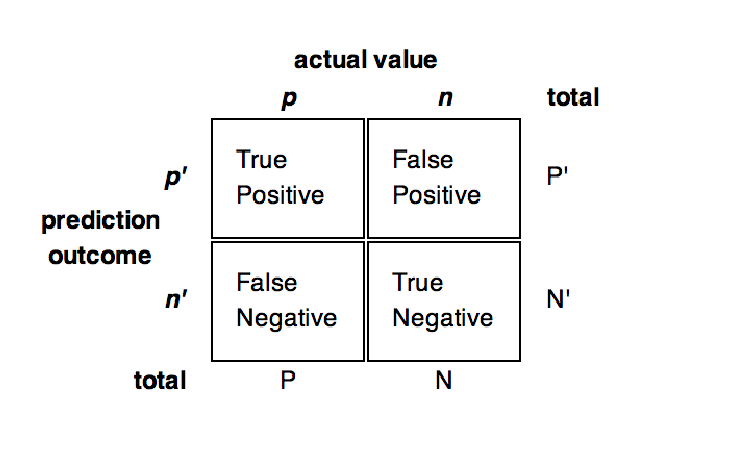
\includegraphics[width=.8\textwidth,height=0.3\textheight]{../images/confMatrix}
  \caption{Predicted vs actual in a 2-class situation}
  \label{class:confMat}
\end{figure}

\newpage

Given the long history and wide application of classifiers there is a plethora of terminology for the key quantities. 

\begin{itemize}
        \item True positive rate (or hit rate, recall, sensitivity)

            
            $$tp\hspace{2mm}rate = \dfrac{Positives\hspace{2mm}correctly\hspace{2mm}classified}{Total\hspace{2mm}positives}$$ 

        \item False positive rate (or false alarm rate)

            
            $$fp\hspace{2mm}rate = \dfrac{Negatives\hspace{2mm}incorrectly\hspace{2mm}classified}{Total\hspace{2mm}negatives}$$ 


         \item Specificity
            
             $$specificity = \dfrac{True\hspace{2mm}cnegatives}{False\hspace{2mm}positives\hspace{2mm}+\hspace{2mm}True\hspace{2mm}negatives} = 1 - fp\hspace{2mm}rate$$

\end{itemize}


             To get a feeling at what these quantities represent, lets just look at a few. \T{sensitivity}, or the \T{true positive rate} is proportion of the actual positives correctly classified as such; and the \T{specificity}, or true negative rate, is the proportion of actual negatives correctly classified as such. So a perfect classifier will be $100\%$ sensitive and $100\%$ specific. You can interpret the other quantities in a similar fashion.
             The reason these quantities can be important, as opposed to another standard model error metric such as \T{RMSE}, is that a model and the associated error never live in a vacuum, i.e. the error should not only give you a metric for model comparison but also convey its accuracy and validity as applied to the situation you are trying to predict or understand. For example, suppose that you are asked to build a classifier whose task it is to predict which amazon user is going to open at least one advertisement email in the next week (for say better email ad targeting). You might find it acceptable to have a model which gives a true positive and true negative rate of $70\%$ because you care equally about sending emails to those who will open and not sending to those who don't. But suppose that next you are asked to build a classifier which is going to predict whether some combination of financial signals should constitute opening a trade position, but you know that the potential loss and gain of any such trade is high. Given that you are likely risk averse you would probably care more that the false negative rate being as low as possible than anything else, i.e. you would be ok with potential missing a good trade but not ok with loosing a large amount.

             Some classification models, such as \T{Naive Bayes}, provide a strict probability for a class given a set of features; otherwise, such as the popular \T{gradient boosting decision tree} classifier, provide a score indicating the level of classification. For example, if you have a two-class problem the output might be on a scale $[a,b]$ where $a$ and $b$ are some numbers close to $0$ and $1$, respectively. Here the classifier simply orders your test cases from those closest to the class $0$ to those closest to the class $1$. Hence, there is no reason to a priori select some threshold such as $.5$ as the cutoff; with every new threshold you will get a new set of classifier error quantities which you can use to understand the general `quality' and robustness of your classifier, as well as an optimal cutoff point. This leads us to \T{Receiver Operator Curves} or \T{ROC}. 

             Given a classifier $\mathcal{C}$, an \T{ROC} take in a threshold value $T$ and returns the tuple (tp rate, tn rate), i.e. 


\begin{align*}
    ROC_{\mathcal{C}}(T) = (fp\hspace{2mm}rate, tn\hspace{2mm}rate), 
\end{align*}


or $ROC_{\mathcal{C}}: [-\inf, \inf] \rightarrow [0,1]\x[0,1]$ which is a curve in the plane. 


There are a couple of points of note here: the point $(0,0)$ indicates that no actual positives have been predicted but no false negatives either, i.e. this point represents the threshold $\inf$ where no $1$'s were predicted; the point $(1,1)$ is the other end of the spectrum, where every point was classified as $1$ resulting in $100\%$ true positive and false positive rate; the point $(0,1)$ represents the perfect classifier, with no points classified as false and no true classification being wrong. In addition, the diagonal represents the random classifier, since we expect it get the same proportion right as it get wrong. Hence, a classifier with an \T{ROC} curve above the diagonal is better than random and below the diagonal is worse than random. 
\begin{figure}
  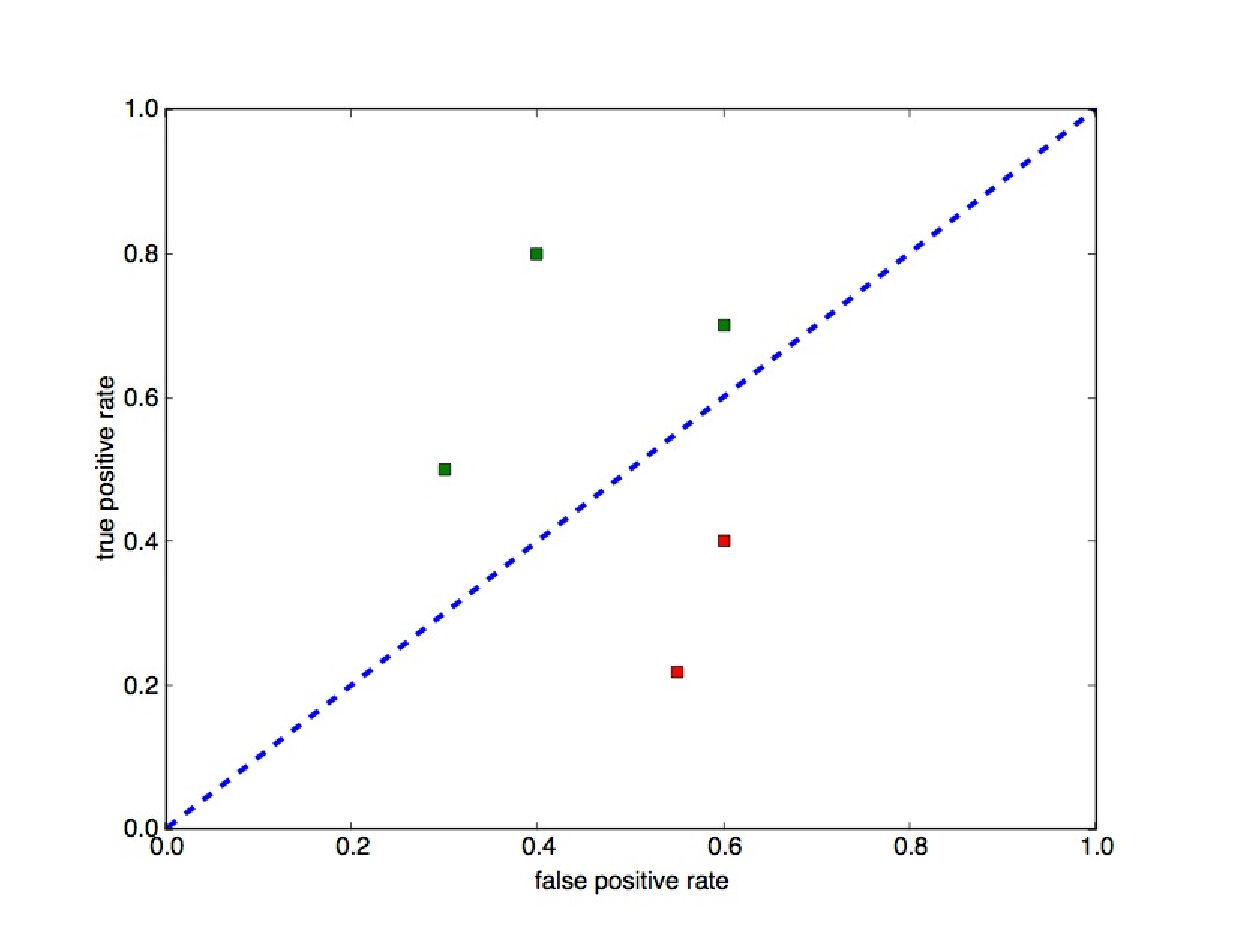
\includegraphics[width=.9\textwidth,height=.45\textheight]{../images/rocRand}
  \caption{The green squares represent classifiers that are better than random and the red squares represent those worse than random}
  %\label{class:confMat}
\end{figure}


By now you can probably guess how to write a simple \T{ROC} algorithm and we take out verbatim from \cite{ROC}. Essentially you order the test cases based on predicted value, from highest to lowest and then start sequentially including the points into the set of positive classifications. With every new point if it is in fact positive you will increase you true positive rate, keeping your false positive rate constant, and if it negative the true positive rate will stay the same while the false positive will increase. Hence, you will either move vertically or horizontally on the plane - lets look at an example below. 

\begin{example}

    Suppose you have a test set of $10$ cases, whose actual class you know, and you classifier outputs the following numbers. The cases are listed below in descending order. 


\begin{center}
    \begin{tabular}{c|c|c}
        \hline
        case & Class(case) & actual \\ \hline
        1 & .97 & True \\ \hline 
        2 & .93 & True \\ \hline 
        3 & .87 & False \\ \hline 
        4 & .70 & False \\ \hline 
        5 & .65 & True \\ \hline 
        6 & .58 & False \\ \hline 
        7 & .43 & True \\ \hline 
        8 & .33 & False \\ \hline 
        9 & .21 & True \\ \hline 
        10 & .05 & False \\ \hline         
    \end{tabular}
\end{center}


\begin{figure}
  \label{class:rocEx}  
  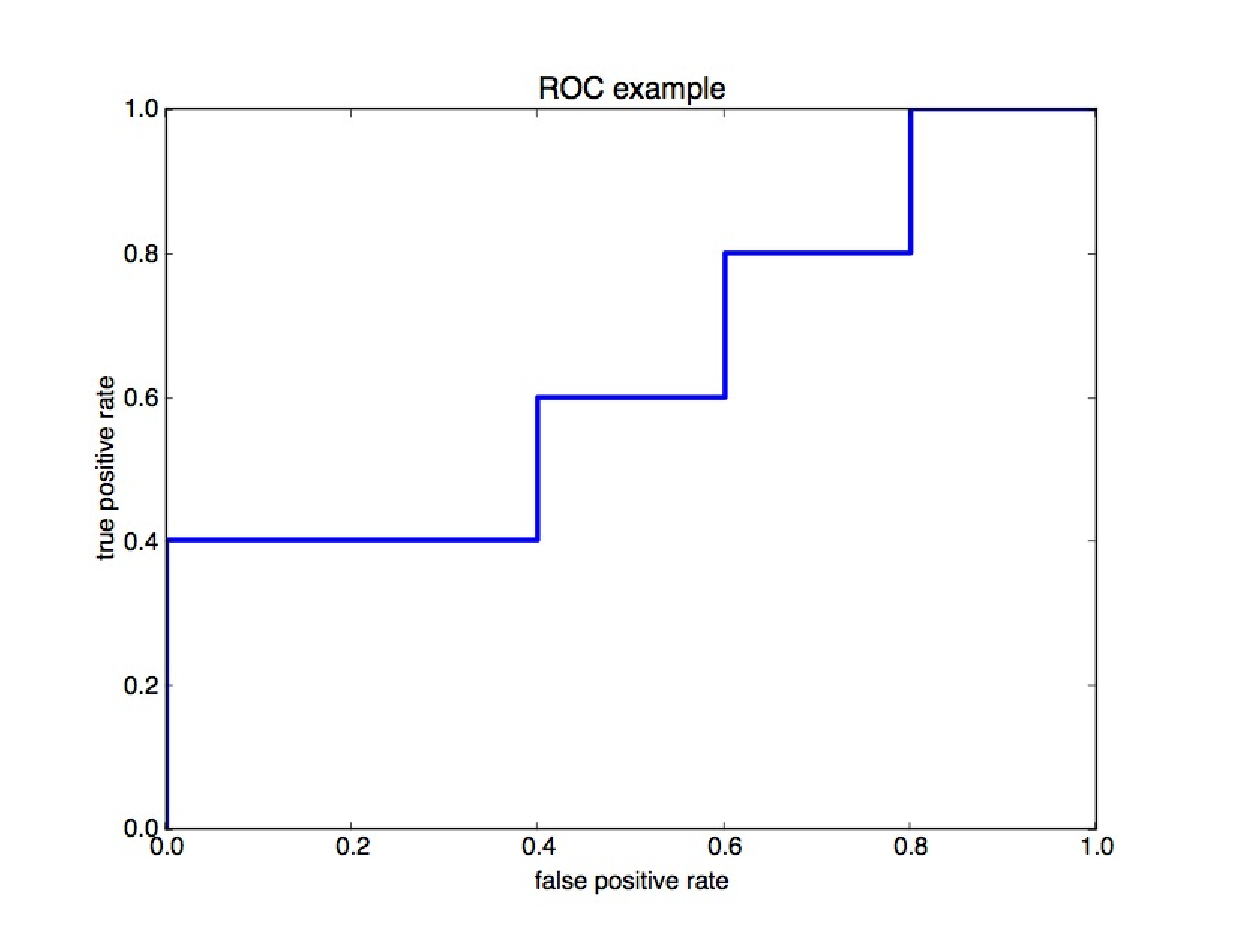
\includegraphics[width=\textwidth,height=.45\textheight]{../images/rocEx}
  \caption{Our example \cal{ROC}}
\end{figure}

With the first threshold, $-\inf$, you classify no cases as true and, hence, have no true or false positives, i.e. the first point on $\mathcal{ROC}$ is $(0,0)$. With the second threshold you will classify the case $1$ as true; since this is correct your true positive rate will now be $\frac{1}{5}$, since there are $5$ positives int the test set, and your false positive rate will be $0$. With the third threshold you will classify cases $1$ and $2$ as true, leading to $\frac{2}{5}$ tp rate and $0$ tn rate, etc In figure \ref{class:rocEx} you can see the $\mathcal{ROC}$ plotted for this example. 
\end{example}



Below is an efficient $\mathcal{ROC}$ algorithm copied verbatim from \cite{ROC}. 

Inputs: $L$, the set of test examples; $f(i)$, the probabilistic classifier's estimate that example $i$ is positive; $P$ and $N$, the
number of positive and negative examples.


Outputs: $R$, a list of $\mathcal{ROC}$ points increasing by fp rate.


Require: $P > 0$ and $N > 0$


\begin{algorithmic}
    \State $L_{sorted} \leftarrow L$ 
    \State $FP \leftarrow TP \leftarrow 0$
    \State $R \leftarrow <>$
    \State $f_{prev} \leftarrow -\inf$
    \While{$i \leq |L_{sorted}|$} 
 \If{$f(i) \neq f_{prev}$} 
 \State push$(\frac{FP}{N}, \frac{TP}{P})$ onto $R$
 \State $f_{prev} \leftarrow f_i$
   \EndIf
   \If{$L_{sorted}[i]$ is a positive example}
      \State $TP \leftarrow TP + 1$
      \Else /* $i$ is a negative example*/
      \State $FP \leftarrow FP+1$
   \EndIf
   \State $i \leftarrow i+1$
\EndWhile
\State push$(\frac{FP}{N}, \frac{TP}{P})$ onto $R$ /* This is (1,1) */
\end{algorithmic}


\section{Other classifiers}


\subsection{Decision Trees}


Decision trees form a fundamental part of the classification, as well as the regression, toolbox. They are conceptually simple and in many instances very effective. 
There are a few basic terms necessary before we dive in: a \T{decision node}, or simply \T{node}, is a place-holder in the tree which signifies a decision being made (in the case of a binary feature, the split will be on whether an item from the data set satisfies the feature conditions); the \T{leaves} of a decision node are class labels. 

The basic algorithm is the following:

\begin{enumerate}

    \item Begin with a decision stump. This is simply a collection of trees consisting of a single node, one for each feature. 
    \item Pick the best one, i.e. given some sort of accuracy measure (\T{splitting objective}) select the single node tree which is the most accurate. 
    \item Check the accuracy of each leaf by evaluating the assigned classification on the associated subset of data. If the accuracy is not sufficiently high, i.e. does not satisfy some pre-defined criteria, continue building the tree as in step 1  utilizing the unused features on the associated subset of data.
\end{enumerate}

Geometrically, decision trees tile your data space with hyper-rectangles, where each rectangle is assigned a class label. There are a number of advantages:

\begin{itemize}

    \item Decision trees are simple and easy to interpret.
    \item They require comparatively little data cleaning (can deal well with continuous, or categorical variables).
    \item Evaluation of a data point is fast, $\log(n)$ where $n$ is the number of leaves.
    \item Can handle mixed-type data.
        
\end{itemize}


The main drawbacks are the following:

\begin{itemize}

    \item Decision trees can easily become complex and lead to over-fitting. One way to deal with this problem is to \T{prune}, by either setting the minimum number of samples for a given node to split (if the min samples is high, the tree is forced to make a decision early, fitting the data less) or by setting the \T{max depth}, limiting the entire size of the tree.
    \item The prediction accuracy can become unstable with small perturbations of the data, i.e. a small ``shift'' can lead to data points falling into the wrong classes. \T{Ensembling} many trees, which we will look at below, can help mitigate this problem.
    \item Finding an optimal tree is NP-complete. Note, that the algorithm described above does not guarantee that a globally optimal tree is found, since it simply makes the best decision at any given node excluding the possibility that say a less than optimal decision locally might lead to a better overall classifier. 
\end{itemize}



For more information about decision trees, see Python's \T{scikit-learn} library. 


        

\subsection{Random Forest}

\T{Random Forest} is a popular ensemble method, whose creation is attributed to Leo Brieman, Adele Culer, Tin Kam Ho, as well as others. The method aims to utilize the flexibility of a single decision tree, while mitigating the drawbacks mentioned above by spreading them out over an entire collection. Random forest, like ensembles in general, can be thought of as a framework more than a specific model. The essential pieces are the following:

\begin{itemize}
    \item The shape of each decision tree, i.e. is the threshold for a single decision a liner, quadratic, or other function.
    \item The type of predictor to use at each leaf; for example, a histogram of constant predictor.
    \item The splitting objective to optimize each node; for example, error rate, information gain, etc.
    \item Some random method which will specify each tree. 
\end{itemize}

For the sake of concreteness, and to set up the some of the technicalities which will help us understand why random forests make sense as an classification approach, lets look at Brieman's original definition and algorithm.
            
\vspace{.3in}

\begin{definition} (Brieman) A \T{random forest} is a classifier consisting of a collection $\{h(X, \theta_k)\}_{k=1, \dots}$ where $\{\theta_k\}$ are independently distributed random vectors and each tree counts a unit vote for the most popular class at input $\overline{x}$.
\end{definition}




For each tree, Brieman specified to do the following:

\begin{enumerate}
    \item Let $N$ be the number of training cases and $M$ the number of features in the classifier. 
    \item Let $m$ be the number of input features that are used to determine the decisions at the tree nodes; $m<<M$. 
    \item Choose a training set of size $n \leq N$, with replacement, and use its complement as a test set. This is know as a \T{bootstrap sample}.
    \item Choose $m$ features which will be used for decisions in the given tree and calculate the best split on those features and training set. 
    \item Let each tree be fully grown, i.e. no pruning. 
\end{enumerate}

The result is a collection of trees $T_{1}, \dots , T_{K}$ where given a input $\overline(x)$ a class can be assigned by taking the mode vote over all the $T_{i}$'s. Note, this was Brieman's original approach; for regression trees, or if you are interested in knowing the strength of a given classification, an average or some other weighted sum can be taken over the outputs of the $T_{i}$'s.


Although $m$ can be determined experimentally, many packages use $\sqrt{M}$ or $log_2(M)$ as default values. 



\subsection{Out-of-bag classification}


Given a collection of \T{bootstrap samples} $T_{1}, \dots, T_{k}$ from a training set $T$, as well as pair $\overline(x), y \in T$, you can use the classifiers trained on samples $T_i$ where  $\overline(x), y \notin T_i$ for measuring the prediction accuracy. For example, suppose you have samples $T_{1}, T_{2}, T_{3}$, and respective trained classifiers $h_{1}, h_{2}$ and $h_{3}$, as well as a pair  $\overline(x), y \in T_{1}$ but  $\overline(x), y \notin T_i$ and  $\overline(x), y \notin T_2$. You can predict the accuracy of your ensemble classifier from evaluating $h_{2}(\overline(x))$ and $h_{3}(\overline(x))$, against the true value $y$. 



This is called an \T{out-of-bag estimate}, or \T{classification}, and empirical evidence has shown that in practice the setup up is as good as using a train/test set of equal size. If your training set is small and you are worried about leaving some part of it out during the model build, this can be a good approach. If your training set is very large, and you are worried about computation time, you can use smaller \T{bootstrap} samples to build a collection of classifiers in less time and ensemble these together. Since the individual classifiers are independent you can make parallelize the whole process making it highly scalable, which can be very useful if you envision having to retrain your models in the same way but on ever growing data sets.  



\subsection{Maximum Entropy}


There are a number of different criteria which you can use to split a decision tree node, and one very popular which we will look at now is called \T{maximum entropy}. You can think of \T{entropy} as the information content, the measure of uncertainty, or randomness of a random variable. 

The \T{entropy} of a random variable $X$ is define as 

\begin{align*}
    H(X) = - \sum_{i \in Class} P(X=i)log_{2}P(x=i)
\end{align*}

where the sum is over all the classes the random variable can output. \ref{class:entropy} shows a plot of what the function would look like for a two-class variable. 

\begin{figure}
  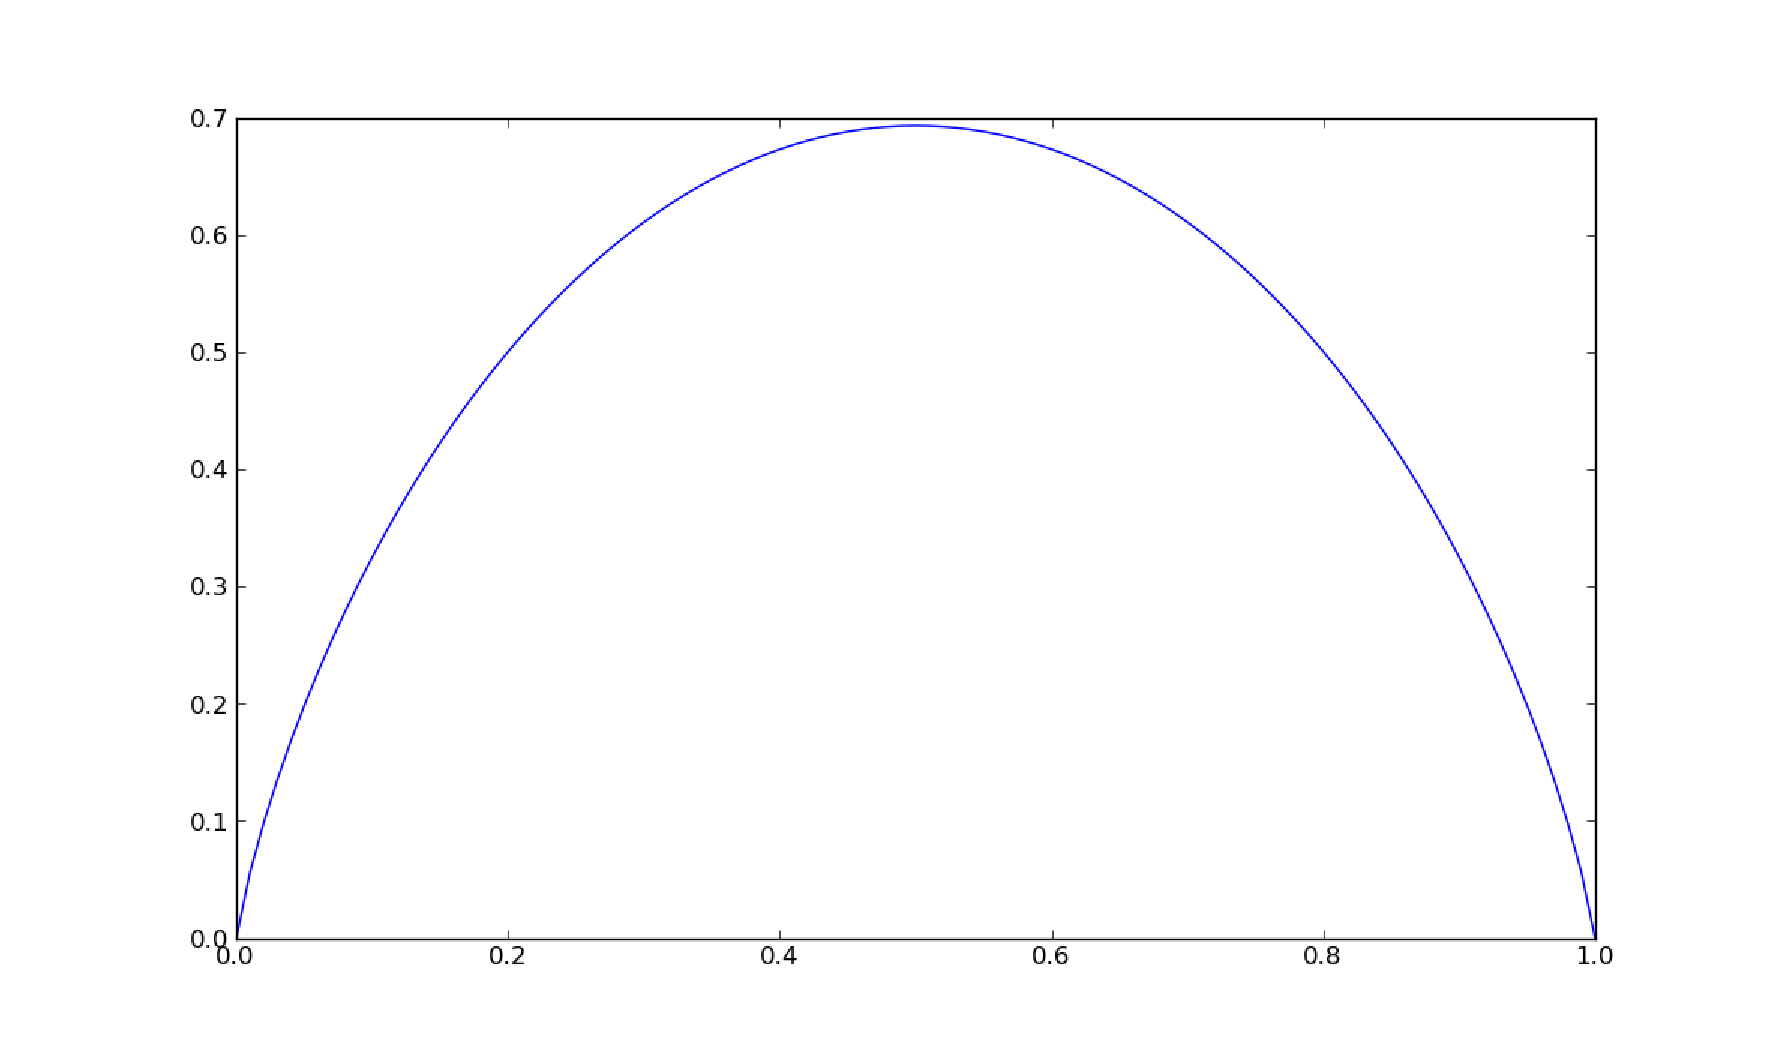
\includegraphics[width=\textwidth]{../images/entropy}
  \caption{The entropy function.}
  \label{class:entropy}
\end{figure}




Lets look at an example to see why this function could make sense. Suppose you are flipping a coin and would like to find a way to measure how biased it is. The probability that the coin flips tails is $p$ and heads is $1-p$. If your coin is highly biased and the probability of heads or tails is $1$ then $H(X)=0$, i.e. the random variable is always there same and has no information content or randomness. If the coin is fair, i.e. $P(X)=.5$ for both heads and tails, then $H(X)=1$, i.e. we have maximum randomness. 


From this example, there are a few intuitive conditions that one might come up with for such a function to exist: a) the function is symmetric and b) has a maximum at $.5$. There is actually one more technical condition which we won't get into here, but the three together ensure that the definition of $H(X)$ is unique up to a constant. If you are interested, in learning more about this I would recommend reading Claude Shannon's wonderful $1948$ paper \textit{A Mathemtical Theory of Communication} where in a tour de force of utter clarity and brilliance he laid out the foundation for information theory, signal processing, and really data science at large.


Back to decision trees\ldots Given a root node and a training set $T$

\begin{enumerate}
    \item calculate the entropy for each feature of your decision tree classifier 
    \item split $T$ into subsets using the feature for which entropy is minimum, i.e. for which we are reducing the randomness of our decision as much as possible
    \item make a decision tree node containing that feature, i.e. split
    \item continue on the above subsets with the remaining features
\end{enumerate}


Another way to say is that at each split we will maximize the \T{information gain} 

\begin{align*}
    IG(f) = H(T) - \sum_{s \in S} p(s)H(s)
\end{align*}

where $H(T)$ is the \T{entropy} of $T$, $S$ the subsets created by splitting $T$ over feature $f$, and $p(s)$ is the proportion of the number of elements in $s$ to the elements in $T$, i.e. the relative size of $s$. The above is known as the $ID3$ algorithm invented by Ross Quinlan. 





\part{Extras}
\chapter{High(er) performance Python}
\label{chapter:performance}
\begin{center}
  {\Large\textit{\\ \vspace{0.1in} - }}
\end{center}
\vspace{0.2in}

To many people, high performance scientific code \emph{must} be written in a language such as C/C++ or Fortran (or even a GPU language).  It is true that these languages will continue to support applications where the highest possible performance is absolutely essential.  For example, some climate simulations can take months of time on a supercomputer, and therefore even a modest 2x speedup of code can make a huge difference.  However, this is not always the case.  In the authors' experience, the time spent writing code (a.k.a. \emph{developer time}) usually far exceeds the time spent waiting for a computer to crunch numbers (a.k.a. \emph{CPU time}).   Since python code is generally easier to write and maintain than e.g. C++, the project goal (e.g. predicting an outcome) can be achieved far quicker and cheaper using Python.  Moreover, Python does not require a developer to mange low-level tasks such as memory allocation, so a non-expert programmer (e.g. a person with a PhD in statistics) can often be used.

The fact that python does not require a programmer to manage memory allocation does not mean that a fundamental understanding of computer engineering will not help.  Used carelessly and without attention to computational limitations, Python can be a very very slow language.

In this chapter we present some basic computer engineering concepts and show how the relate to Python performance.  We also present a number of practical examples of what can be done to increase performance of your code.

\section{Memory hierarchy}
One can think of a computer as a machine that takes data from disk and transfers it to a CPU.  The CPU, which is composed of a control unit, arithmetic logic unit, and more, transforms this data, which is then written back to disk or displayed to the user.  The term \emph{memory hierarchy} refers to the hierarchical storage scheme for data.  See figure \ref{performance:fig:heirarchy1} for a simplified version that shows memory getting smaller and faster (in terms of the time needed to access it) as you get closer to the CPU core.  In figure \ref{performance:fig:heirarchy1} we measure time in CPU clock cycles.  The CPU clock is a source of electrical pulses that synchronize CPU operations.  As of 2013, typical laptop CPU clocks operate at 2-3 billion cycles per second (GHz). The reasons why the larger memory is slower has to do with a combination of economics and physics and is beyond the scope of this text.  Note that the actual memory hierarchy is more complicated with multiple levels of cache and registers (figures \ref{performance:fig:pyramid}, \ref{performance:fig:heirarchy3}).).

\begin{figure}
  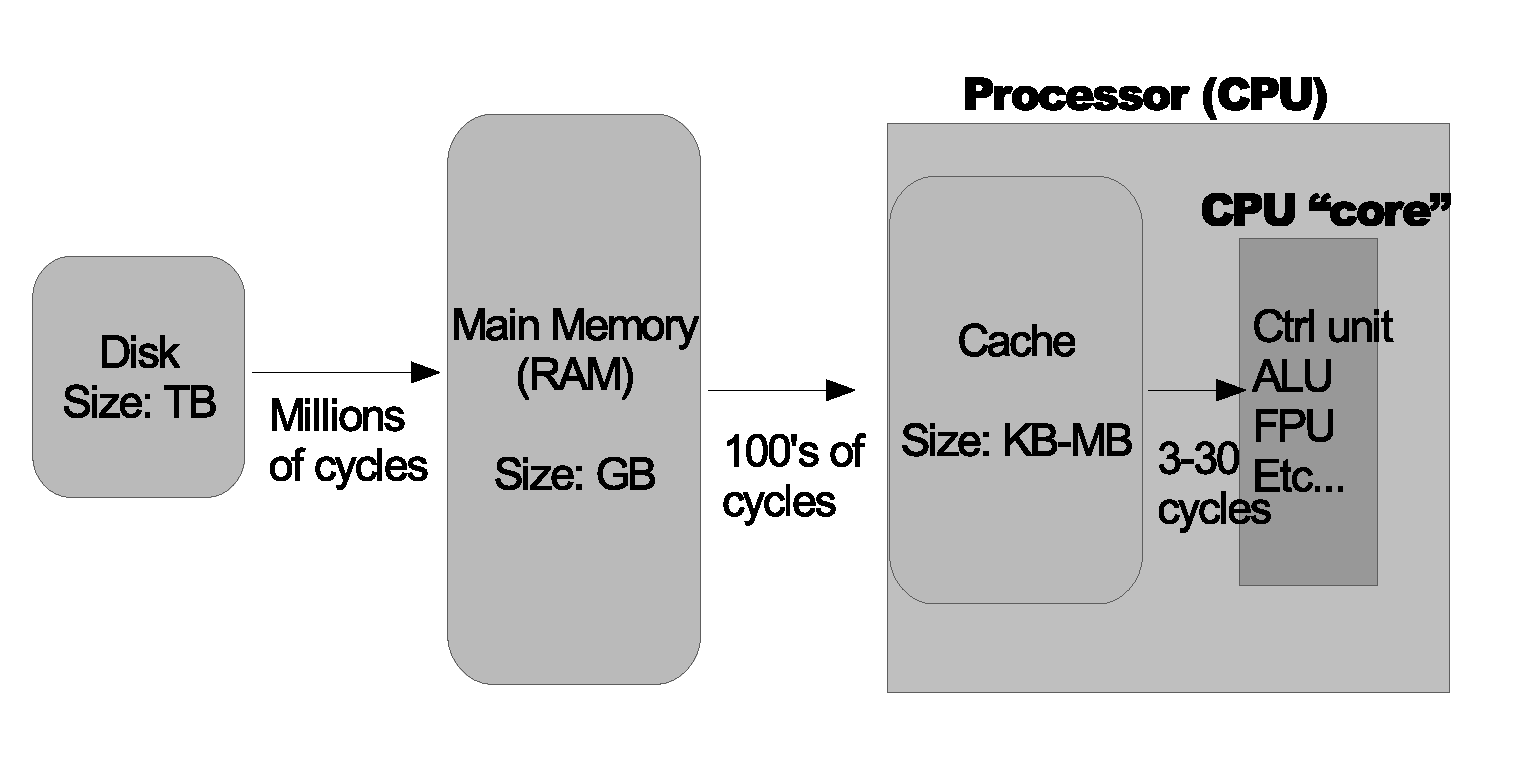
\includegraphics[width=0.9\textwidth]{../images/memory_heirarchy}
  \caption{Simplified memory hierarchy showing disk, main memory (RAM), cache, the computer components they are situated in, and the time (in clock cycles) needed to move data between them.}
  \label{performance:fig:heirarchy1}
\end{figure}
\begin{figure}
  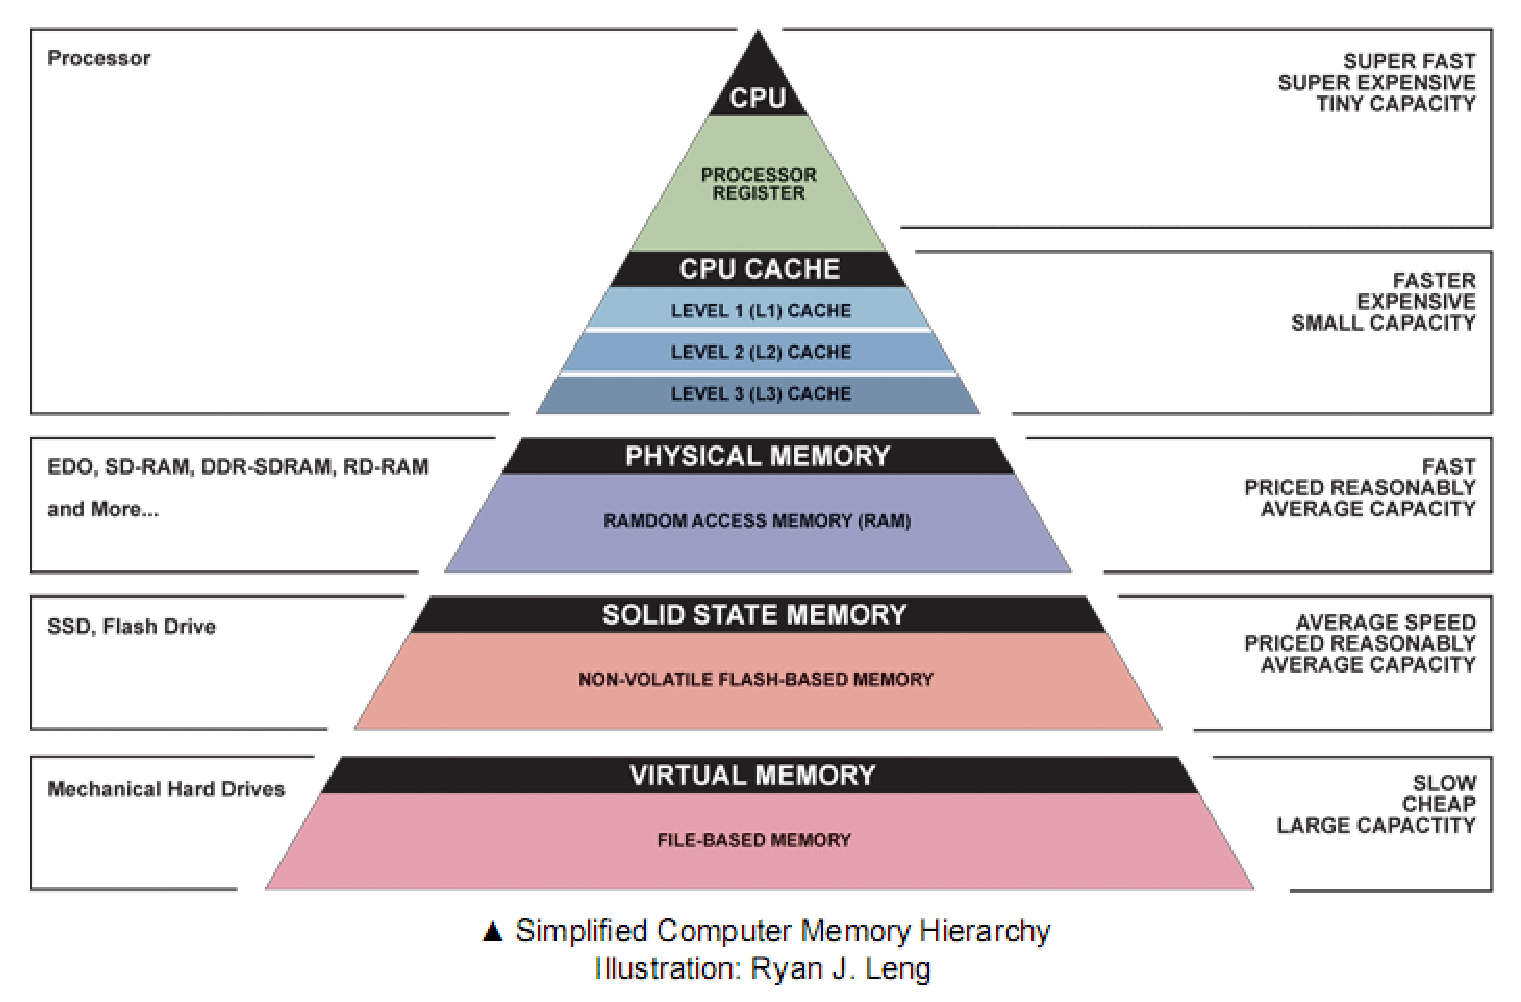
\includegraphics[width=0.85\textwidth]{../images/hei}
  \caption{Memory hierarchy with more detail.}
  \label{performance:fig:pyramid}
\end{figure}
\begin{figure}
  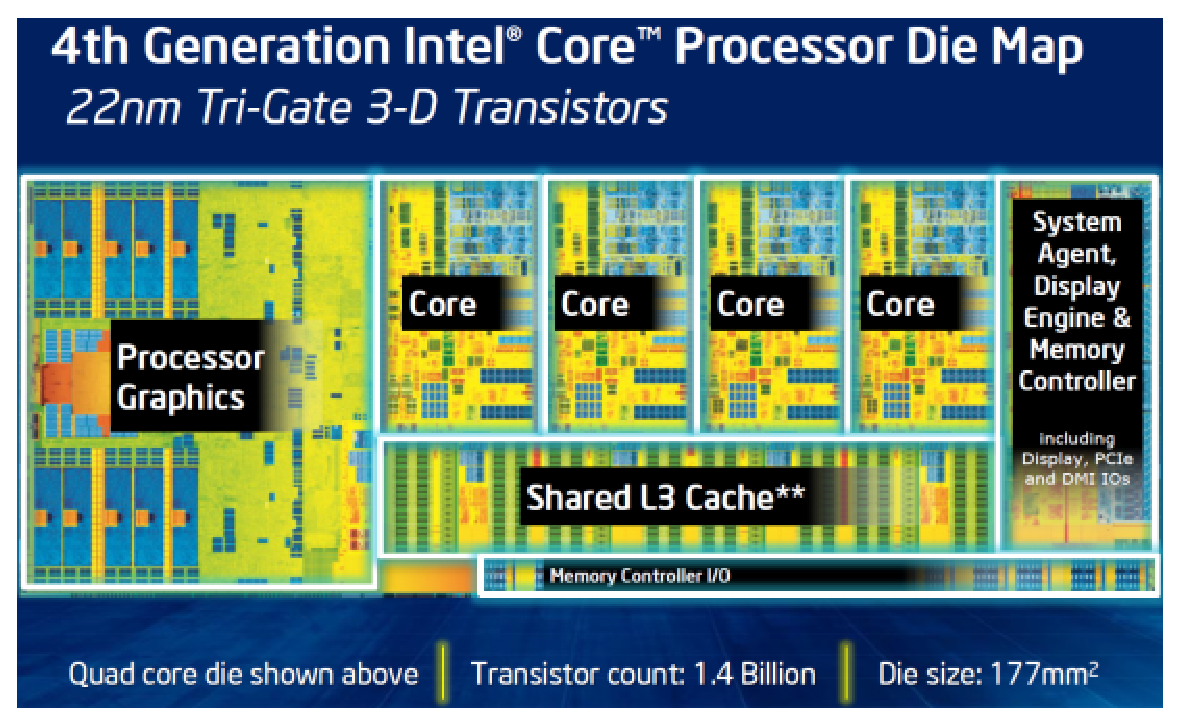
\includegraphics[width=0.85\textwidth]{../images/haswelldiemap_550}
  \caption{Picture of an Intel core i7 chip showing shared L3 cache.  L1 and L2 cache as well as registers are located on the CPU core.}
  \label{performance:fig:heirarchy3}
\end{figure}
What you need to keep in mind is that if the slower component cannot supply the faster upstream component with data, then we have a bottleneck.  This \emph{memory wall} can only be avoided with one of two means.  First, the faster upstream component can make repeated use of its data.  For example, you can load a training data set from disk into memory and use it to train a logistic regression.  The loading of the data is slow because of the disk access.  However, this happens only once, and then (for at least a few minutes) the data is repeatedly used in an optimization procedure.  The access time difference between main memory and cache can be mitigated in a similar manner.  
% TODO Put in a gemm example
Take for example the \emph{axpy} operation $z = ax + y$ where $x$ and $y$ are vectors and $a$ is a scalar.  It often happens that $x$ and $y$ are too large to fit in cache.  One wrong way to deal perform the axpy would be to first load as much of $x$ as possible into cache, multiply it by $a$, then send that result back to memory and load the next bit of $x$ in.  After we had multiplied $ax$, we could start loading both $ax$ and $y$ into cache and add them.  A smarter implementation loads smaller chunks of $x$ and $y$ so that they fit into cache.  We then multiply the chunk of $x$ by $a$ and then add it to that chunk of $y$.  This ``double usage'' of $x$ avoids one cache-memory load and speeds code up the axpy operation significantly.

%A similar phenomenon happens with main memory and cache.  Take for example computing the dot product between two vectors $x\cdot y = \sum_ix_iy_i$.  If the vectors both fit into cache, then we can load both into cache, multiply them together, then add the result.  If however they do not fit, it makes sense to divide $x$ and $y$ into $n$ length $m$ chunks such that each chunk of $x$ and $y$ fit into memory together.  We can then do the dot product on every chunk independently and then add the result.  For example, writing the first $x$ chunk as $(x_{11},\cdots,x_{1m})$, and the $n^{th}$ we $(x_{n1},\cdots,x_{nm})$, we then decompose the dot product as:
%\begin{align}
%  x\cdot y &= \left( x_{11}y_{11} + \cdots x_{1m}y_{1m} \right) + \cdots + (x_{n1}y_{n1} + \cdots x_{nm}y_{nm}).
%  \label{performance:align:dotprod}
%\end{align}
The second means to avoid a memory wall is to slow down the CPU clock.  Since the clock runs slower, the slower components take less CPU cycles to do their work, and thus less cycles are wasted.  This by itself does not help performance.  However, the slower clock speeds consume far less power, and allow more cores (each with their own cache) to be placed on chip.  The overall performance increases, but comes at the cost of added complexity (programmers need to design parallel algorithms).  This sort of clock-slowing became more-or-less inevitable when (for years) CPU clock speeds increased at a much higher rate than memory bus speeds.

One final note on memory.  While the casual programmer generally thinks very little about main memory vs. cache vs. registers, he or she absolutely needs to be aware of disk versus main memory.  If your computer cannot fit all data in main memory, it will use a portion of the disk, called \emph{swap space} as a kind of pseudo memory.  Since reading/writing to and from disk is exceptionally slow, this practice of \emph{swapping} can significantly slow down all operations on your computer.  This can crash servers.  For this reason, it is your responsibility to keep track of memory usage.  While all machines have built in utilities that do this, the ``best'' one is \T{htop}\footnote{\T{htop} does not work on all versions of mac.  There are \T{htop} installers, but sometimes the memory usage just doesn't make sense.}  In Ubuntu you can install with \T{sudo apt-get install htop}.  You can start the utility by typing \T{htop} in the command prompt.  In addition to monitoring memory usage, \T{htop} allows you to see CPU usage, kill processes, and search for processes.

\begin{figure}
  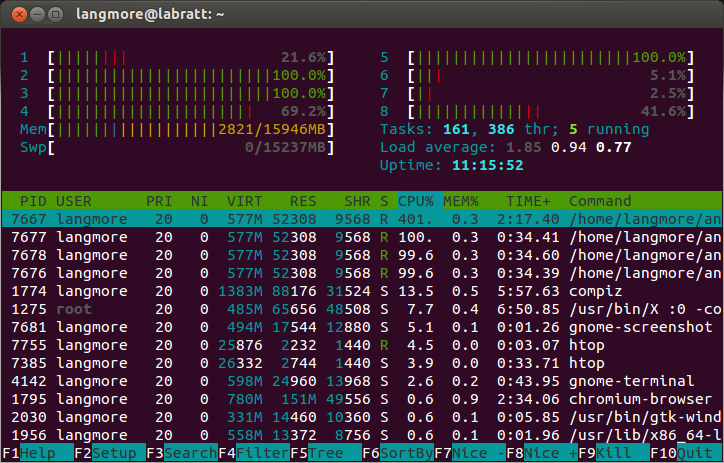
\includegraphics[width=\textwidth, clip=True, trim=0 100 0 0]{../images/htop}
  \caption{Screenshot of \T{htop} invoked on a laptop with 4 cores and 4 virtual cores (so it appears as 8 cores to the OS).  Notice that multiple cores are in use due to a multi-threaded numpy matrix multiply.  You can also see that 2821 MB of memory is currently in use.  The green memory and CPU usage is ``normal usage'', and red indicates ``kernel usage'', in other words, the OS kernel is invoking this.  The most common example of a red CPU line is due to a disk read/write.}
  \label{performance:fig:htop}
\end{figure}

A useful number to keep in mind when calculating memory usage is to realize that double precision numbers (the default for Python if your system is 64 bit) take up 64 bits, which is 8 bytes.  So an array of numbers that has length 1 million is 8 million bytes, or, 8 MB.

\section{Parallelism}

Since, as we saw above, performance gains will not come through increasing the clock speed in the serial pathway of figure \ref{performance:fig:heirarchy1}, it is now coming through parallelism.  Suppose you have a processor with 4 cores and wish to perform the axpy operation $z = ax + y$.  A starting point could be to divide the memory address range of $x$ and $y$ into four chunks, and send each chunk to a different core.  Each core performs an axpy on each chunk, and then writes the result to the appropriate space in memory (so that the end result is a contiguous array $z$).  If each chunk fits perfectly into each core's cache, and our memory controller can handle these four operations efficiently, then we should see a four-times speedup!  This sort of operation is known as \emph{embarrassingly parallel} because it did not involve communication between the separate cores.

As another example of an embarrassingly parallel algorithm, consider the random forest.  In this case we have $n$ independent trees, each being fit independently (see figure \ref{performance:fig:RF}).
\begin{figure}
  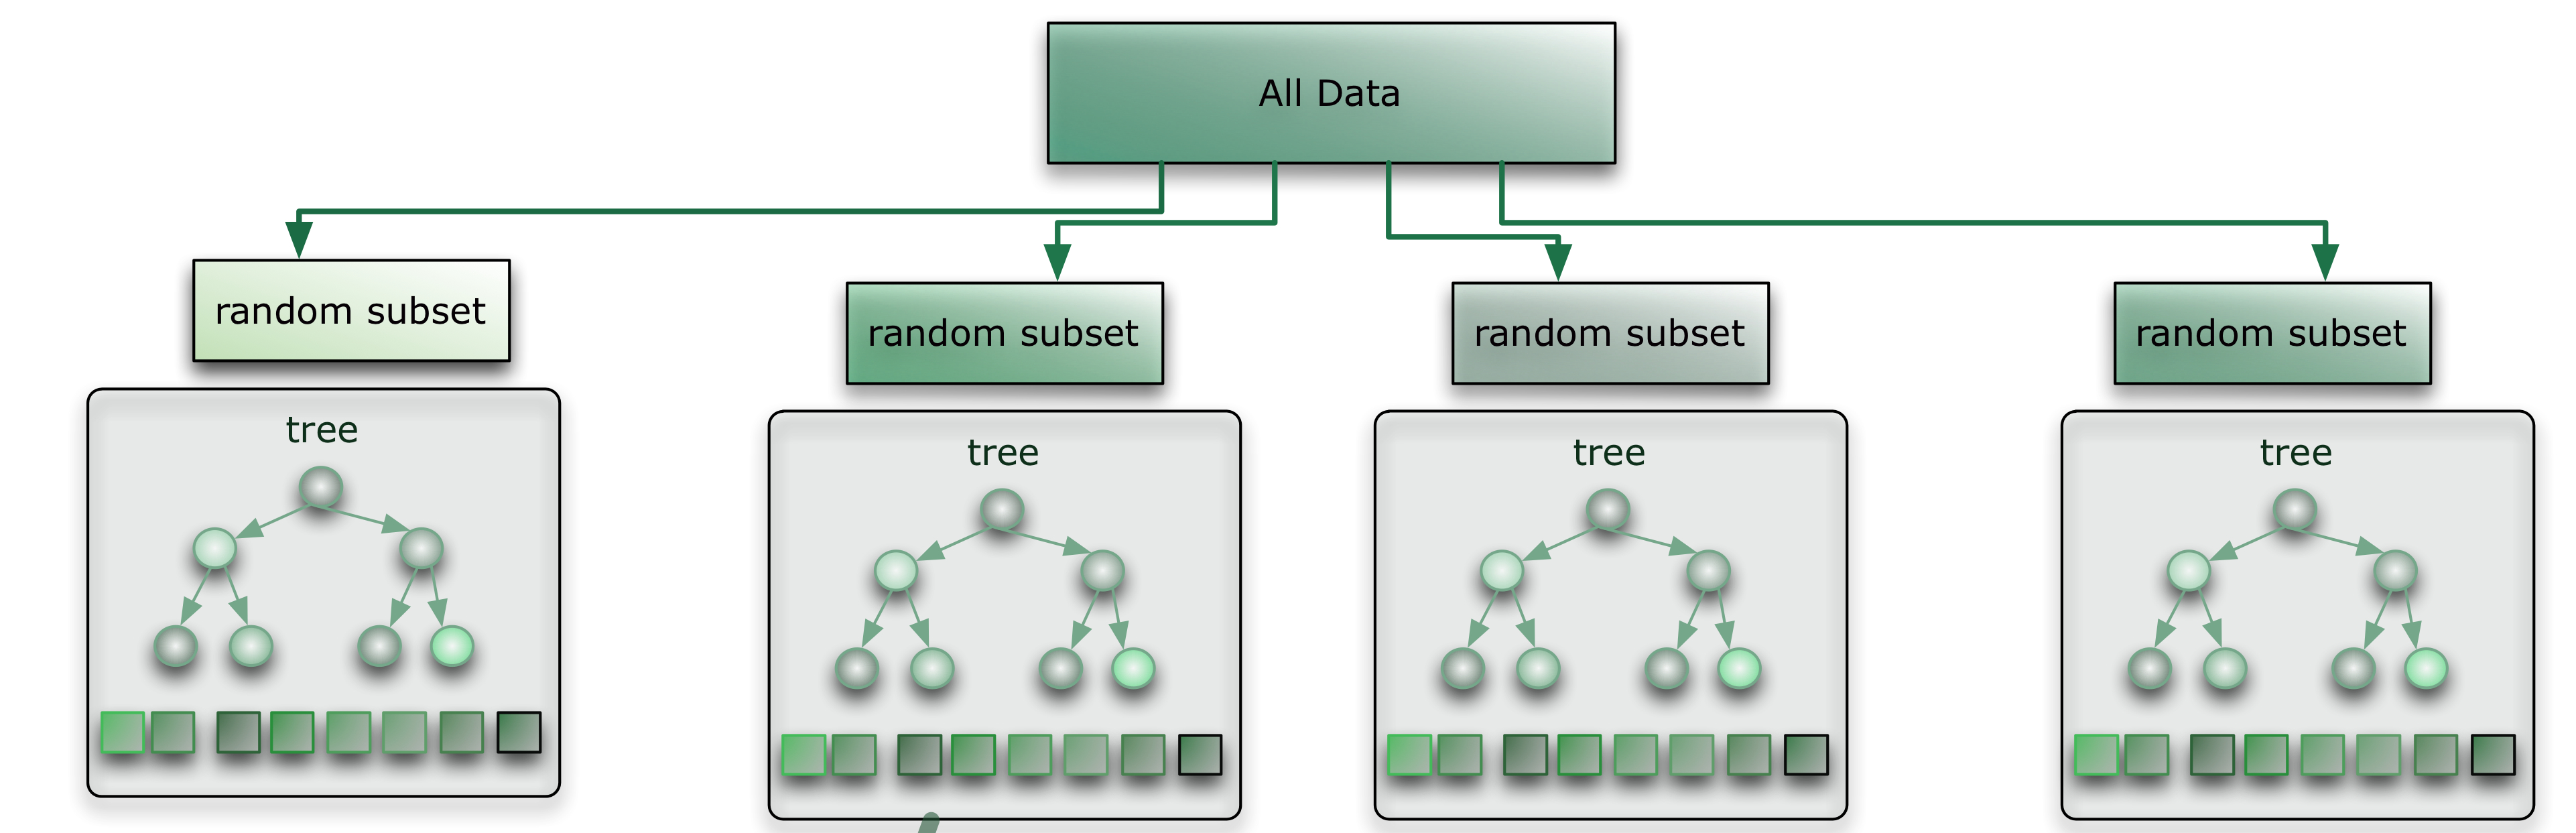
\includegraphics[width=\textwidth]{../images/RF}
  \caption{Random forest is an embarrassingly parallel algorithm.}
  \label{performance:fig:RF}
\end{figure}

As an example of an algorithm that is not embarrassingly parallel, consider solving the system $Ax = b$.  As mentioned in \ref{linear:subsection:numerical}, for medium to large systems this is usually done with algorithms that repeatedly multiply $A$ by different vectors $v$, and then add this result to another vector $w$.  Suppose our machine has two cores.  Then each multiplication can be decomposed as:
\begin{align}
  \label{performance:align:matvec}
  \left( 
  \begin{matrix}
    A_{11} & A_{12}\\
    A_{21} & A_{22}
  \end{matrix}
  \right)
  \left( 
  \begin{matrix}
    v_1\\
    v_2
  \end{matrix}
  \right)
  =
  \left( 
  \begin{matrix}
    A_{11}v_1 + A_{12}v_2 \\
    A_{21}v_1 + A_{22}v_2
  \end{matrix}
  \right)
\end{align}
The first core can handle $A_{11}v_1 + A_{12}v_2$ and thus assemble the top rows of $Av$.  The other core can handle the bottom rows.  However, each result must be sent to the location where the corresponding chunk of $w$ is being kept so that we may compute $Av + w$.  This process repeats many times, and during each repetition, the result must be shared between cores.  This \emph{communication} incurs some overhead, both in terms of programming time and cpu cycles.

More important (at least to our intended audience) than communication overhead is the increase in complexity that comes with parallelizing a program.  Because of this, and the fact that some algorithms cannot be parallelized, large portions of your code will likely remain serial (= not parallel).  If 50\% of your code is serial, then even if you have 1000 cores you can only achieve 50\% speed-up.  This fact is generalized in \emph{Amdahl's law} (see figure \ref{performance:fig:amdahl}).
\begin{figure}
  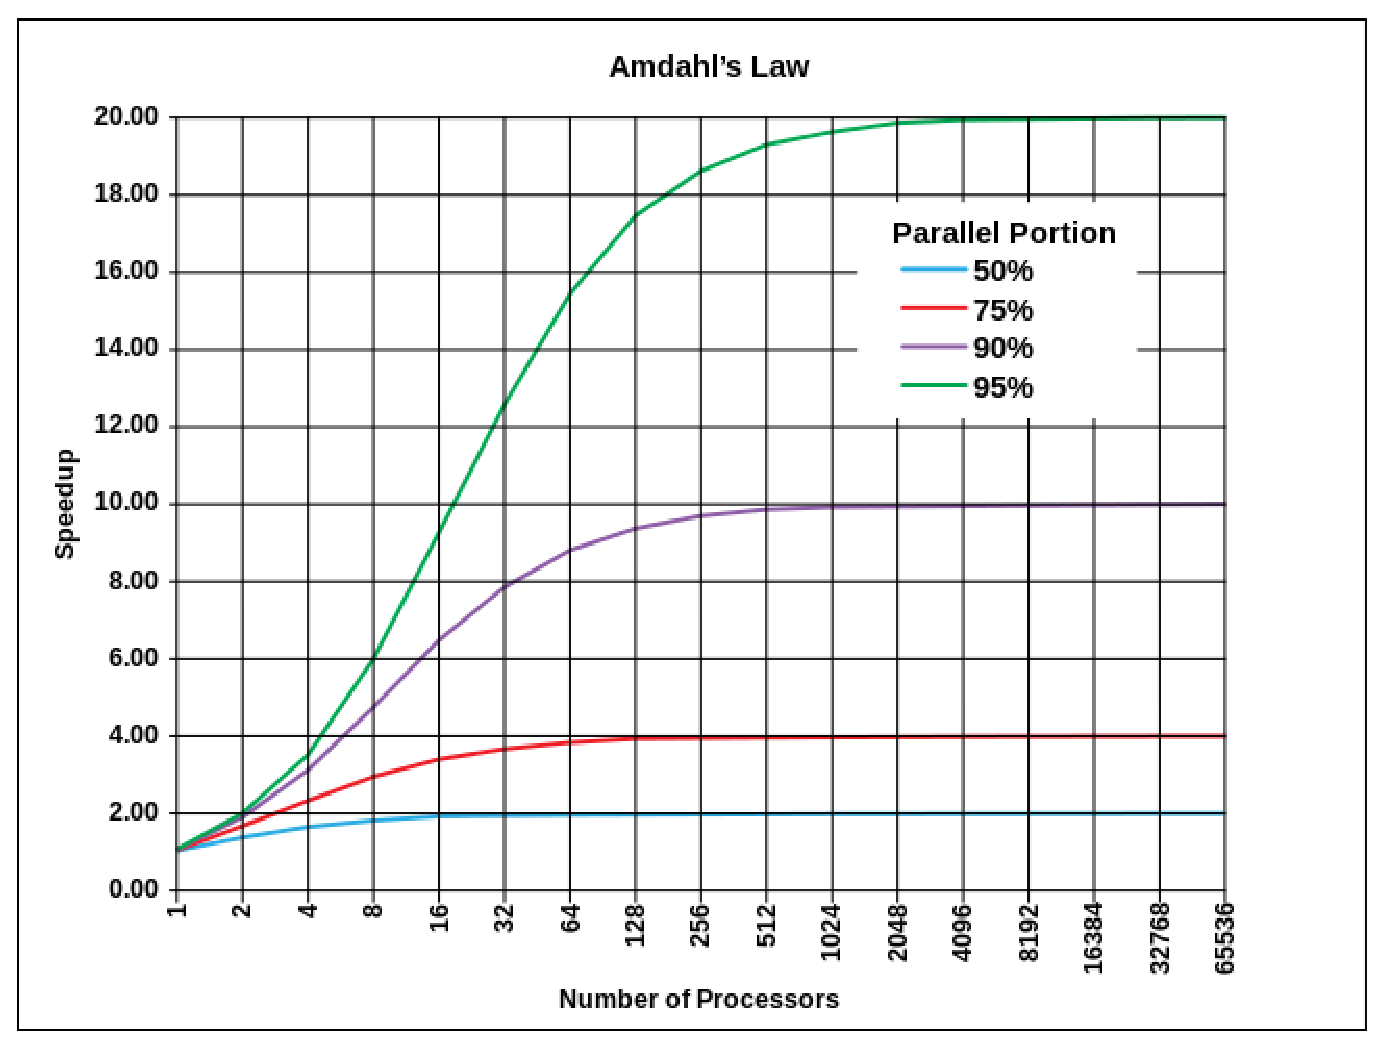
\includegraphics[width=0.5\textwidth]{../images/AmdahlsLaw}
  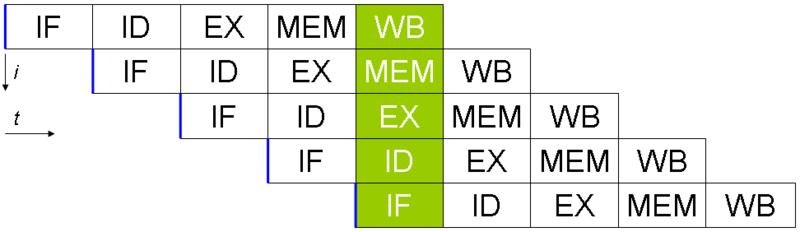
\includegraphics[width=0.5\textwidth]{../images/800px-Fivestagespipeline}
  \label{performance:fig:amdahl}
  \caption{Left:  Amdahl's law states that the fraction of code that is serial places limits on the speedup that parallelization can achieve.  Right: A canonical five-stage pipeline in a RISC machine (IF = Instruction Fetch, ID = Instruction Decode, EX = Execute, MEM = Memory access, WB = Register write back)--cut-and-paste from Wikipedia.}
\end{figure}

It is important to realize that these parallel tasks can be performed by both \emph{processes} and \emph{threads}.  A process is a new ``program'' that is started.  When you start the Firefox web browser, you are starting a new process.  That process has access to its own space in memory.  Python provides support for starting processes through the \emph{subprocess} and \emph{multiprocessing} modules (more on that later).  Since these processes have their own memory space, any data used by them must be copied into that space.  So, for example, if separate processes handled each of the two blocks in \eqref{performance:align:matvec}, then each process would need a \emph{copy} of the data needed to perform that multiplication.  For example, one process would need a copy of $A_{11}$, $A_{12}$, and $v$, and the other process would need a copy of $A_{21}$, $A_{22}$, and $v$.  This can result in unfortunate increase in total memory used.  There are multiple ways to copy data between processes.  In Python, the preferred method is to \emph{serialize} it with the \emph{cPickle} module (turn it into a byte stream) and send using stdin and stdout.  In contrast, multiple \emph{threads} can share a memory space.  This saves memory and eliminates communication overhead.  Threads however are more restricted in what they can do.  For example, if you have two threads running in a Python program, then only one is able to execute code at a time!  This is due to the Global Interpreter Lock (GIL).  This means that multi-threading in Python is very low performance.  

A common library for multi-threading is the Open-MP library.  Due to the GIL, multi-threading directly in Python is not usually done, but libraries such as numpy execute C/Fortran code \emph{outside} of Python and thus avoid the GIL.  In this way, numpy is able to perform parallel programming such as matrix-vector multiplications through multi-threading (thus avoiding the overhead of spawning new processes).  The most popular and versatile multiprocessing library is the Message Passing Interface (MPI).  This library provides a number of ways to start new, and communicate between, processes.  It also provides a number of so-called \emph{reduction} operations whereby data stored on multiple processes is ``reduced'' to one single number.  For example, if each process holds a segment of an array, a possible reduction would involve computing the sum of all the numbers in the array.  The processes each can sum their respective sub-arrays, and then send their result to the master processes, which adds all the sub-sums.  Although MPI is in wide use, it does not provide ways to restart failed tasks.  When you have less than say 100 computers, this is not a big deal.  When however you are Google and regularly perform jobs using thousands of machines, this is important.  For that reason, the \emph{MapReduce} paradigm was developed.  MapReduce allows \emph{mapping} of tasks to individual processes (located on different machines).  It then provides support for different types of reduction as well as restarting of failed tasks.  Hadoop is an open source implementation of MapReduce.  Despite the popularity of Hadoop/MapReduce, it is important to realize that this is a highly restrictive method of parallel computing with a huge overhead required to spawn new processes.

\section{Practical performance in Python}

In this section we introduce you to a few common means to increase the performance of your Python programs.

\subsection{Profiling}

Python code is meant to be easy to understand and maintain.  It is generally \emph{not} good practice to optimize (for performance) everything since this often results in less straightforward code.  To quote Donald Knuth, ``We should forget about small efficiencies, say about 97\% of the time: premature optimization is the root of all evil.''  When you do optimize, the proper first step is to \emph{profile} first.  Profiling is the practice of examining the time taken by different sections of code.  This helps you find the bottlenecks.  You then optimize these bottlenecks.

The easiest way to profile a script is with the unix \T{time} utility.
\begin{minted}{bash}
\$ time python myscript.py

real	0m24.332s
user	0m47.268s
sys	0m0.792s
\end{minted}
The \T{real} line is the total \emph{wall time} of the process invoked directly by the script.  This is the time you would measure if you brought out a stopwatch and timed until the process was finished.  The \T{user} number is the total user CPU time.  In the above case, the script launched a master process, which in turn started two slaves (three processes total).  The master was idle for most of the time, and the slaves worked most of the time.  Therefore, the \T{user} time was about twice the \T{real} time.  The \T{sys} line is the time spent in system calls, such as I/O.

IPython provides a very nice interface to the \emph{timeit} module, which we explain with figure \ref{performance:fig:timeit_1}. In IPython, the timeit module runs the code following the command \T{timeit} (or sometimes, \T{\%timeit} is necessary) a number of times until it has a good estimate of the time needed for it to run.  
\begin{figure}
  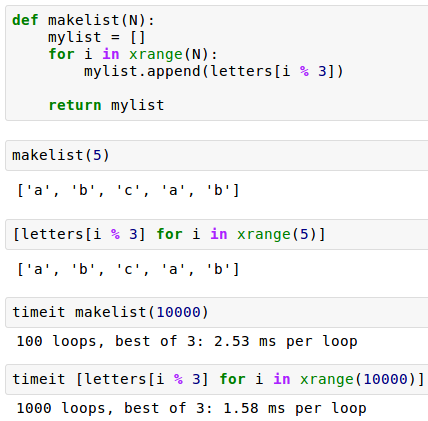
\includegraphics[width=0.7\textwidth]{../images/timeit_1}
  \caption{Figure illustrating use of the timeit module.}
  \label{performance:fig:timeit_1}
\end{figure}
Figure \ref{performance:fig:timeit_1} shows that creating a simple list with 10,000 elements takes about 50\% longer in a for loop than with a list comprehension.  See section \ref{performance:subsection:rulesofthumb} for an explanation of this difference.  Note that \T{timeit} can also be run with the options \T{-n} and \T{-r} which determine the number of iterations used to determine the time the function call takes.

While \T{timeit} can be used to test small snippets of code, it is not the best tool to test larger functions.  The \T{line\_profiler} is the authors' preferred method.  It provides a readout of time spent in each line of a function.  The \T{line\_profiler} can be installed with \T{\$ pip install line\_profiler}.  The easiest way to use the \T{line\_profiler} is to follow these steps (see also listing \ref{performance:listing:lineprofiler}):
\begin{enumerate}
  \item Wrap your code in a function, and then put an \T{@profile} decorator at the top of the function.
  \item Run this function with some command line argument.  This is usually done by writing a script that calls the function (either a unit test, or some script you are using to help run your code).  This script can even be the same module as the function, where you have written ``run capabilities'' into a \T{if \_\_name\_\_ == '\_\_main\_\_':} clause.  
  \item Supposing the script is called \T{myscript.py}, call the script with the command line argument:  \T{kernprof.py -l myscript.py}.  The \T{-l} argument invokes line-by-line profiling\ldots and you will get funny errors if you don't use \T{-l}.
  \item View the results with \T{python -m line\_profiler myscript.py.lprof}.  This prints the results to stdout, so it is often useful to pipe them to \T{less}.
\end{enumerate}
\begin{listing}
  \begin{minted}{python}
import numpy as np

def pythondot(list1, list2):
    dotsum = 0
    for i in xrange(len(list1)):
        dotsum += list1[i] * list2[i]
    
    return dotsum

def numpydot(arr1, arr2):
    return arr1.dot(arr2)

@profile
def testfuns(arrsize, numiter):
    mylist = [1] * arrsize
    myarray = np.ones(arrsize)

    for i in xrange(numiter):
        temp = pythondot(mylist, mylist)
        temp = numpydot(myarray, myarray)

if __name__ == '__main__':
    testfuns(1000, 10) 
  \end{minted}
  \caption{Profiling various dot products with the \T{line\_profiler} module (see also figure \ref{performance:fig:lineprofiler}).}
  \label{performance:listing:lineprofiler}
\end{listing}
\begin{figure}
  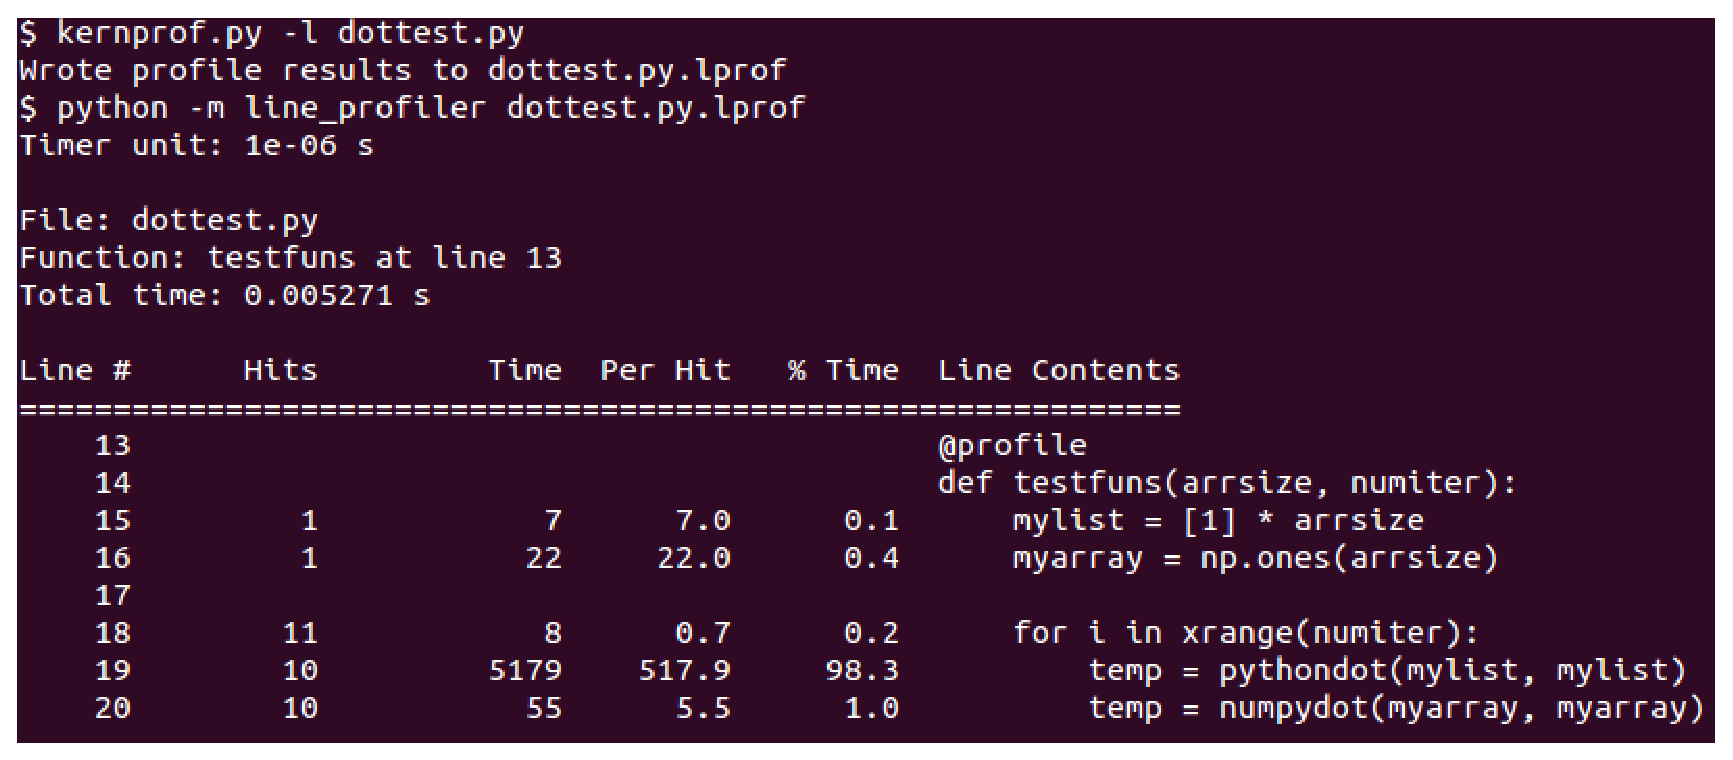
\includegraphics[width=\textwidth]{../images/dottest_profile}
  \caption{Results of profiling session, viewed with less.  See also listing \ref{performance:listing:lineprofiler}.}
  \label{performance:fig:lineprofiler}
\end{figure}
The profile results show the percentage time spent in each function (this is usually the first place I look), the number of times each function was called, and the time spent in each function.  The output in figure \ref{performance:fig:lineprofiler} shows that the pure-python for-loop dot product is much much slower than a numpy dot product.

\subsection{Standard Python rules of thumb}
\label{performance:subsection:rulesofthumb}
Here we go over some standard Python performance tricks and rules of thumb.  These are ``standard'' in the sense that most developers know of them.

\subsubsection{List comprehensions and map}
As evidenced in figure \ref{performance:fig:timeit_1}, a list comprehension is often faster than an explicit for loop.  The reason for this is that a list comprehension handles the append step in an optimized manner.  Thus, if you have a for loop so simple that the appending of an item to a list takes a significant amount of the time, you can get around 50\% speedup.  This 50\% (or so) speed up usually does not merit a pizza party.  So don't be tempted to wrap every for loop into a list comprehension.  This type of code would be unreadable.  A good rule of thumb is this:  If a for loop is not slowing anything down (suppose it is only over a few items), then a for loop is usually more readable and is preferred.  Use a list comprehension only if the list comprehension can be put in one 79 character line.  The \T{map} function is an alternative to list comprehensions.
\begin{minted}{python}
mylist = ...# create a list

def myfun(item):
    ...# do something
    return new_item

# same as [myfun(item) for item in mylist]
myresults = map(myfun, mylist)
\end{minted}

\subsubsection{Hash tables}
Another, sometimes huge, performance tip (that should always be followed) is to take advantage of the fast hash-table lookup capabilities of Python's \T{set} and \T{dict} objects.  Suppose you create a dictionary \T{mydict = \{'name': 'ian', 'age': 13\}}.  A \emph{hash table} is created that stores the keys ``name'' and ``age.''  These keys are not stored as the actual strings.  Instead, they are transformed using a \emph{hash function} to a location in a table.  Many different keys could be transformed to the same location, but it is very very unlikely that this will happen to you.  So you can safely assume that in \T{mydict}, the keys ``name'' and ``age'' are mapped to different locations.  The values (or rather, pointers to the values) are stored at these locations.  So, when I write \T{mydict['name']}, Python uses a hash function to transform ``name'' to a location, and in that location is the string ``ian.''  See figure \ref{performance:fig:hash}.  The performance significance is that, no matter how long your dictionary is, it takes the same amount of time to find a key in it.  For comparisons sake, you could (and many novices do) implement a slow dictionary by storing two lists, one with the keys and one with the values.  Note that a \T{set} is also stored as a hash table (with no values, other than an indication that the element is in the set), so finding items in a set is also fast.  See figure \ref{performance:fig:hash_test}
\begin{figure}
  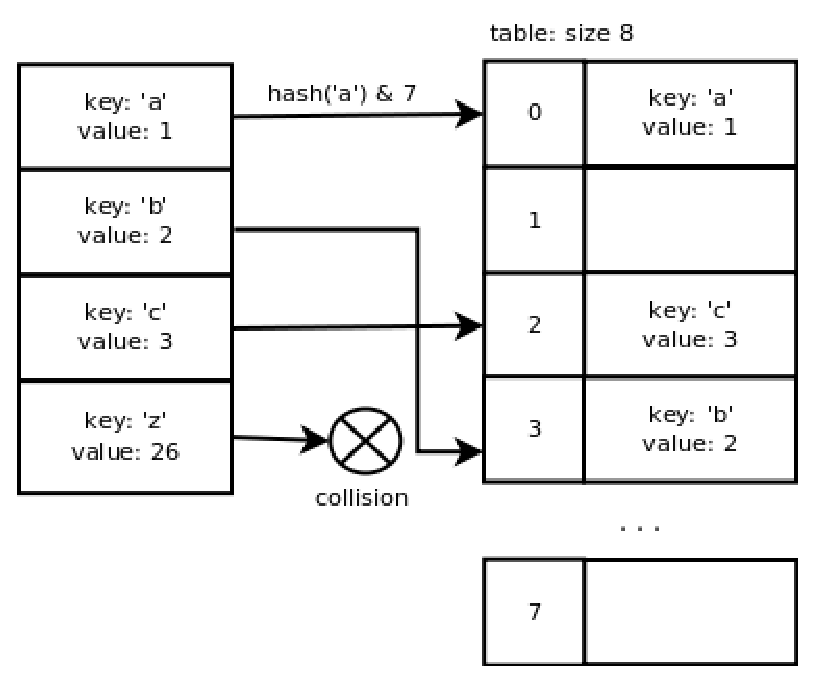
\includegraphics[width=0.75\textwidth]{../images/hash}
  \caption{A hash table corresponding to the dictionary \T{\{'a': 1, 'b': 2, 'c': 3, 'z': 26\}}.  In this table, both \T{'a'} and \T{'z'} were mapped to the same table entry, so there was a collision.  In reality, this is very very rare.}
  \label{performance:fig:hash}
\end{figure}
\begin{figure}
  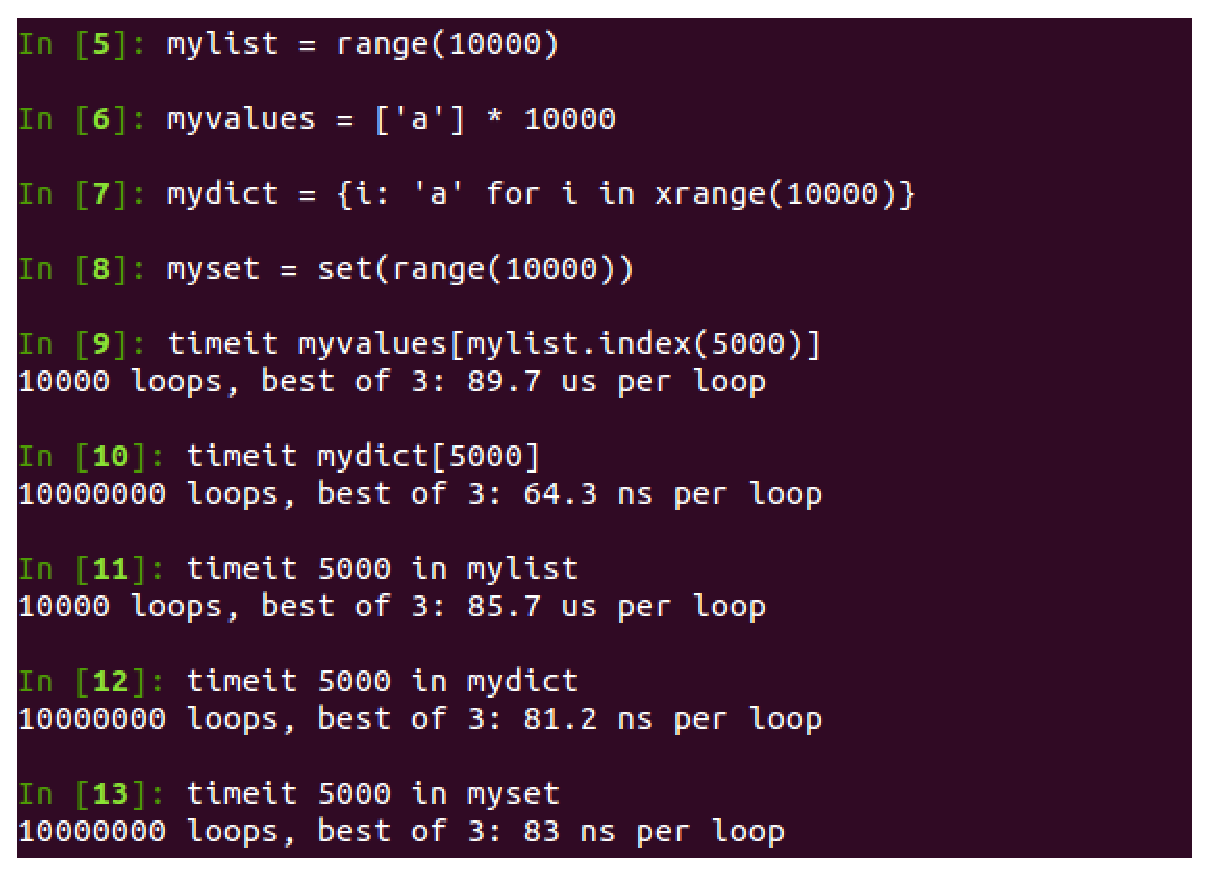
\includegraphics[width=0.85\textwidth]{../images/hash_test}
  \caption{A performance test showing where a hash table is 1000 times faster than list lookup.  Note that \T{mydict} will be a dictionary with keys equal to the numbers 0 through 9999, and every value equal to 'a'.   The calls \T{myvalues[mylist.index(5000)]} and \T{mydict[5000]} both return the 5000th entry in mylist/mydict (equal to 'a' in both cases).  The list version is 1000 times slower because \T{mylist.index(5000)} searches through the list, entry-by-entry, for the number 5000.  The last three calls are boolean tests, each returning \T{True}.}
  \label{performance:fig:hash_test}
\end{figure}

\subsubsection{Iterators}
Consider the following code:
\begin{minted}{python}
mylist = ... # Create a list
for i in range(N):
    mylist[i] = mylist[i] + 10    
\end{minted}
This steps through a list and modifies it.  We use another list, namely \T{range(N)}, to provide an iterator \T{i} to help us step through.  The first time through \T{i=0}, the second \T{i=1} and so on.  You can access the iterator by setting (try it!) \T{myiter = range(10).\_\_iter\_\_()}.
\begin{minted}{python}
>>> mylist = range(10)  # Create a list
>>> myiter = mylist.__mylist__.iter()
>>> myiter.next()
0
>>> myiter.next()
1
\end{minted}
This is more-or-less what happens when you use \T{for in range(10):} to do ten iterations of some task.  This is somewhat wasteful however since we never actually need the entire list at once.  All we need is some way to step through the numbers that would have been in the list.  This same ends can be achieved by replacing \T{range} with \T{xrange}.  The speed difference between using \T{range} and \T{xrange} is small, but the memory savings can be significant and it is generally good practice in Python 2.7 to use \T{xrange}.  \footnote{Note that in Python 3.0+ \T{range} will automatically be converted to \T{xrange} inside for loops, and \T{xrange} will no longer be used\ldots.  So if you want your code to be Python3.0+ compliant, use \T{range}.}

In general, an \emph{iterator} is an object with a directed one-dimensional structure and a \T{next()} method that allows us to iterate through that structure.  A \T{list} is an \emph{iterable} since it can be converted to an iterator.  A \emph{generator} is an iterator that is tied to a function (so that some function is called to provide the next element).

List comprehensions can be replaced with expressions that produce iterators that have a \T{next()} method.
\begin{minted}{python}
>>> mylist = ['a', '0', 1, 'b']
>>> mygen = (item for item in mylist if item.isalpha())
>>> mygen.next()
a
>>> mygen.next()
b
>>> mygen.next()
Traceback (most recent call last):
  File "<stdin>", line 1, in <module>
StopIteration
\end{minted}

A common use of iterators that we have made extensive use of is the file object.
\begin{minted}{python}
>>> f = open('myfile.txt', 'r')
>>> f.next()
'this is the first line\n'
>>> f.next()
'this is the second line\n'
\end{minted}
Note that you could read the entire file into memory at once using \T{f.read()} or \T{f.readlines()}.  This however is often a very wasteful use of memory.

\begin{exercise}
  Consider the following code fragment that loops through using an explicit index:
  \begin{minted}{python}
mylist = ... # Create a list
mysum = 0
for i in xrange(len(mylist)):
    mysum += mylist[i]
  \end{minted}
In contrast, consider this method of looping, which does not use an index:
  \begin{minted}{python}
mylist = ... # Create a list
mysum = 0
for item in mylist:
    mysum += item
  \end{minted}
  The second method works if \T{mylist} is replaced by an iterator, but the first method does not, why?  

  Note that this is a reason the second method is preferred.  If you also need the index, then try using \T{for i, item in enumerate(mylist)}.
\end{exercise}

\subsection{For loops versus BLAS}
\label{performance:subsection:forblas}

As figure \ref{performance:fig:lineprofiler} shows, dot products are much faster in numpy than in pure Python.  The reason that numpy is fast is that it uses some version of the Basic Linear Algebra Subprograms (BLAS).  BLAS is a library of linear algebra functions, mostly written in Fortran.  It takes advantage of your machine's cache configuration, and some versions support multi-threading.  The version of BLAS that comes with standard numpy is 5 - 50 times slower than an optimized version, so the user is encouraged to upgrade to a version that is built with an optimized BLAS (i.e. Intel's Math Kernel Library (MKL)).  This is easy to do if you are using Continuum's Anaconda or Enthought's EPD.  There are many reason's that Python for loops are slow.  Consider the following loop:
\begin{minted}{python}
mylist = ... # Create a list

mysum = 0
for item in mylist:
    mysum += item
\end{minted}
Since Python is not compiled, the python interpreter needs to convert this code into machine code every time through the loop.  Moreover, since a list can contain a very wide variety of objects, Python needs to figure out how to add these objects (or if they even can be added) every time through.  Python also checks if you are using a value of \T{i} that is outside the bounds of \T{mylist}.  None of these checks need to be done with numpy arrays since they are of pre-determined shape and data type.  Note that it is \emph{not} efficient to use a for loop on a numpy array (in fact, it is often slower than a list).  Numpy is only optimal when you call the built-in numpy functions (e.g. \T{sum}, \T{dot}, \T{max}) that call external BLAS libraries.

\subsection{Multiprocessing Pools}
Many embarrassingly parallel tasks can be thought of as applying a function to a list, and getting back another list.  Consider first the following (serial) code:
\begin{minted}{python}
mylist = ...# create a list

def myfun(item):
    ...# do something
    return new_item

# same as [myfun(item) for item in mylist]
myresults = map(myfun, mylist)
\end{minted}
So long as \T{myfun(mylist[i])} is independent of \T{myfun(mylist[j])}, this code could be parallelized by 
\begin{enumerate}
  \item Splitting \T{mylist} up into chunks
  \item Sending each chunk to a separate worker process (hopefully attached to a separate processor core)
  \item Letting each process handle its chunk, creating a shorter version of \T{myresults}
  \item Send the results back to the master process, which re-assembles it.
\end{enumerate}
The following code does just that:
\begin{minted}{python}
from multiprocessing import Pool

# Start 4 worker processes
pool = Pool(processes=4)
myresults = pool.map(myfun, mylist)
\end{minted}

If you use \T{pool.map()}, the workers complete their work, then return the results.  This can cause memory issues if the results are large.  A variant is \T{pool.imap()}, which creates an iterator such that results are sent back as soon as they are available.  See section \ref{performance:subsection:stream-processing-text} for more details and an example.

\subsection{Multiprocessing example:  Stream processing text files}
\label{performance:subsection:stream-processing-text}

A common data science task is to read in a large file (that does not fit into memory), compute something with every line (e.g. count word occurrences), and write the results to a new file.  The proper way to do this is to read the file in  line-by-line and process each line one at a time.  This avoids blowing up your memory, and is parallelizable (see below).  

\subsubsection{Serial examples}
An example is the following:
\begin{minted}{python}
def process_line(line):
    # Write some code here
    return newline

with open('myfile.txt', 'r') as f:
    with open('outfile.txt', 'w') as g:
      for line in f:
          newline = process_line(line)
          g.write(newline)
\end{minted}
A closely related problem would be that of opening many small text files, computing something in each, and printing results to a new file.  As a concrete example, consider the case where we have a collection of files and want to count the occurrences of nouns in them.  To detect nouns requires some non-trivial (and often slow) NLP.  This means that the processing function is likely the bottleneck.  In that case it makes sense to parallelize things.  Let's start with the serial version of this program.

\rule{\textwidth}{2pt}
\begin{minted}{python}
import nltk
from os import listdir
from os.path import isfile, join
import sys


def main():
    basepath = '/home/langmore/jrl/enron/data/raw/enron-spam/all'
    allfiles = [f for f in listdir(basepath) if isfile(join(basepath, f))]

    # The part of speech that we will keep
    pos_type = 'NN'

    for filename in allfiles:
        result = process_file(pos_type, basepath, filename)
        sys.stdout.write(result + '\n')


def process_file(pos_type, basepath, filename):
    """
    Read one file at a time, extract non stop words that whose part of speech
    is pos_type, return a count.

    Parameters
    ----------
    pos_type : String
        Some nltk part of speech type, e.g. 'NN'
    basepath : String
        Path to the base directory holding files
    filename : String
        Name of the file

    Returns
    -------
    counts : String
        filename| word1:n1 word2:n2 word3:n3
    """
    path = join(basepath, filename)

    with open(path, 'r') as f:
        text = f.read()
        tokens = nltk.tokenize.word_tokenize(text)
        good_words = [t for t in tokens if t.isalpha() and not is_stopword(t)]
        word_pos_tuples = nltk.pos_tag(good_words)
        typed = [wt[0] for wt in word_pos_tuples if wt[1] == pos_type]
        freq_dist = nltk.FreqDist(typed)

        # Format the output string
        outstr = filename + '| '
        for word, count in freq_dist.iteritems():
            outstr += word + ':' + str(count) + ' '

        return outstr


def is_stopword(string):
    return string.lower() in nltk.corpus.stopwords.words('english')


if __name__ == '__main__':
    main()
\end{minted}
\rule{\textwidth}{2pt}
Notice how in the above code the I/O is all in \T{main()}, and the processing is all in \T{process\_file()}.  This is the standard ``good practice'' of separating interface from implementation.  We have also made the choice (again, good standard practice) to push the processing to a function that deals with one single file at a time.  This sort of choice is usually necessary for parallelization.

\subsubsection{Parallel example}

We now write a parallel implementation.  We will use the \T{Pool} class from the \T{multiprocessing} package.  This provides an easy way to parallelize embarrassingly parallel programs.  \T{Pool} launches a ``pool'' of workers, and automatically divides up the work among them.  The ``work'' must be passed to them in the form of an iterable such as a list.  It is meant to mimic the functionality of the \T{map()} function.  There is one issue with this however in that \T{map()} will get all results at once, and all the results may be too big to fit in memory.  So instead we use a multiprocessing version of \T{imap}.  \T{imap} returns an iterator that allows us to step through the results one-by-one as they become available.  There is an additional parameter \T{chunksize} that specifies the size of chunks to send to/from the workers at one time.  

It will re-use the functions \T{process\_file()} and \T{is\_stopword} verbatim, so we don't re-write them here.  The \T{main()} function is significantly changed and now supports both single and multiprocessing modes.  There is an additional function \T{imap\_wrap()}, along with a couple of re-definitions, which are necessary if we want to exit with \T{Ctrl-C} rather than explicitly killing the process with \T{ps}.

\rule{\textwidth}{2pt}
\begin{minted}{python}
import nltk
from os import listdir
from os.path import isfile, join
import sys

import itertools
from functools import partial
from multiprocessing import Pool
from multiprocessing.pool import IMapUnorderedIterator, IMapIterator


def main():

    basepath = '/home/langmore/jrl/enron/data/raw/enron-spam/all'
    allfiles = [f for f in listdir(basepath) if isfile(join(basepath, f))]

    # Number of slave processes to start
    n_procs = 2

    # The size chunk to send between slave and master
    chunksize = 10

    # The part of speech type that we will keep
    pos_type = 'NN'

    # Construct a function of one variable by fixing all but the last argument
    # f(filename) = process_file(..., filename)
    f = partial(process_file, pos_type, basepath)

    # Construct an iterator that is equivalent to
    # (f(filename) for filename in allfiles)
    #
    # If we are using 1 processor, just use the normal itertools.imap function
    # Otherwise, use the worker_pool
    if n_procs == 1:
        results_iter = itertools.imap(f, allfiles)
    else:
        worker_pool = Pool(n_procs)
        results_iter = worker_pool.imap_unordered(f, allfiles, chunksize=chunksize)

    for result in results_iter:
        sys.stdout.write(result + '\n')


def imap_wrap(func):
    """
    Wrapper for Pool.imap_unordered that allows exit upon Ctrl-C.  This is a fix
    of the known python bug  bugs.python.org/issue8296 given by 
    https://gist.github.com/aljungberg/626518
    """
    def wrap(self, timeout=None):
        return func(self, timeout=timeout if timeout is not None else 1e100)
    return wrap

# Redefine IMapUnorderedIterator so we can exit with Ctrl-C
IMapUnorderedIterator.next = imap_wrap(IMapUnorderedIterator.next)
IMapIterator.next = imap_wrap(IMapIterator.next)
\end{minted}

\rule{\textwidth}{2pt}
It is instructive to run this script on a large collection of files while monitoring \T{htop}.  We see that each core is able to spend most of its time with a full green bar.  This indicates that they are being fully used.  If chunksize is too large, then one core will end up with significantly more work to do, and this slows things down.  This is only really a problem when you're working with a small number of files, and so this doesn't matter.  If chunksize is too small, you risk burdening the processes with the task of pickling and communicating.  No kidding here!  There are many cases where a small chunksize can result in performance that gets worse as you add more cores.  For the files on my computer at this time, \T{chunksize = 10} was a decent compromise.  In any case, you simply must test out the time with a few different settings to make sure you get some speedup.  This can be done with \T{time python streamfiles.py > /dev/null}.  The redirection sends the output \T{/dev/null}, which is a ``file'' that is erased as soon as it is written.  In other words, you never see the output.

\subsection{Numba}

\subsection{Cython}





\backmatter
\include{glossary}
\include{notat}
\bibliographystyle{amsalpha} %The style you want to use for references.
\bibliography{../../bibliography}
%\bibliography{mr,bibliography} %The files containing all the articles and books you ever referenced.
\printindex %Make an index AUTOMATICALLY

\end{document}











%%%%%%%%%%%%%%%%%%%%%%%%%%%%%%%%%%%%%%%%%%%%%%%%%%%%%%%%%%%%%%%%%%%%%%%%%%%%%%
%%   Notes that were in this template when I got it.
%%%%%%%%%%%%%%%%%%%%%%%%%%%%%%%%%%%%%%%%%%%%%%%%%%%%%%%%%%%%%%%%%%%%%%%%%%%%%%
\input{chap1/sec12}
When LaTeX sees a line like \input{chap1/sec11}, it looks for the file sec11.tex in the directory chap1 and inputs this file line by line into appdatasci.tex. (The file sec11.tex is the contents of my Section 1.1 of my book.) Again, don't use \begin{document} or \end{document}: sec11.tex should contain just the exposition of this section.

Finally, a couple of comments about bibliographies. Especially near the start of your careers, when you start writing papers and theses, I advise you strongly to create a file called bibliography.bib which contains like this:


@ARTICLE{EGG:96a, %A code of your own making by which you refer to this paper
AUTHOR = "Edgar G. Goodaire and D. A. Robinson",
TITLE = "A construction of loops which admit right alternative loop rings",
JOURNAL = RESUM, %RESUM is defined in mr.bib; it expands to an official journal name
YEAR = {1996},
VOLUME = {59},
PAGES = {56--62} }

@UNPUBLISHED{EGG:98,
AUTHOR = "Edgar G. Goodaire and D. A. Robinson",
TITLE = "Commutative alternative rings: A construction",
NOTE = "preprint"

@BOOK{EGG:99a,
AUTHOR = "Edgar G. Goodaire and Sean May and Maitreyi Raman",
TITLE = "The {M}oufang Loops of Order less than $64$",
PUBLISHER = "Nova Science Publishers, Inc.",
ADDRESS = "Commack, New York",
YEAR = {1999}
Each time you want to reference something, if it is not in your bibliography.bib, you must add, with formatting as above. YOU DO THIS ONLY ONCE IN YOUR LIFE. Ever thereafter, if you want to reference Goodaire and Robinson in your paper, you write \cite{EGG:96a}. After you latex master.tex, you bibtex master.tex. At this point, the bibtex program will go into your bibliography.bib file and pull into your paper or book just those references which you require in your current work. Run latex master.tex once (or twice) more and look at the output. Your references will be numbered and alphabetized automatically and all the references in your exposition will be just as you want them.

The file mr.bib is a short version of mrabbrev.bib, which is available from the AMS (if it isn't on our own systems). It's a list of all official abbreviations for journals and is invaluable.
The command \bibliographstyle{amsalpha} asks bibtex to use the amsalpha style. There are numerous other possibilities. Many book publishers have their own. There is much much more to all this than I can outline here. I do urge you, however, to read the sections in Lamport's book which deal with bibliographies (and making your index). Good luck.
